\documentclass[aps,floatfix,10pt,amssymb,amsfont,amsmath,superscriptaddress,float,nofootinbib,longbibliography,nobalancelastpage,twocolumn]{revtex4-2}
\usepackage{graphicx} % Required for inserting images
\usepackage{xcolor}
\usepackage{booktabs}
\usepackage{array}
% --- MISSING FIGURE FILES -------------------------------------------
% The numerics PNGs (b6r30eta10.png etc.) were not supplied with the
% source.  \missingfig draws a labelled placeholder box in their place.
% TO RESTORE THE REAL FIGURES: drop the .png files next to main.tex and
% replace \missingfig{...} with \includegraphics[width=...]{...} in the
% four figure environments of Appendix A.2 (Numerics).
\newcommand{\missingfig}[2][0.3]{%
  \fbox{\begin{minipage}[c][2.8cm][c]{#1\linewidth}%
  \centering\footnotesize\ttfamily #2\\[4pt]\normalfont\itshape figure file not supplied%
  \end{minipage}}}
% --------------------------------------------------------------------
\usepackage{hyperref}
\hypersetup{hidelinks}
\usepackage{braket}
\usepackage{amsfonts}
\usepackage{amssymb}
\usepackage{amsmath}
\usepackage{bbm}
\usepackage{bm}
\usepackage[english]{babel}
\usepackage{amsthm}
\newtheorem{theorem}{Theorem}
\newtheorem{lemma}{Lemma}
\newtheorem{duplicate}{Theorem}
\newtheorem{corollary}{Corollary}
\newtheorem{remark}{Remark}
\newtheorem*{lemma*}{Lemma}
\usepackage{subfig}
\usepackage{tikz}
\usetikzlibrary{arrows,positioning}
 \usetikzlibrary{quotes}
\usetikzlibrary{shapes.geometric,arrows.meta,calc,fit,backgrounds}
\usepackage{yquant}
\pgfdeclareshape{yquant-multictrlshape}{
   \inheritsavedanchors[from=yquant-circle]%
   \foreach \anc in {center, north, north east, east, south east, south, south west, west, north west} {%
      \inheritanchor[from=yquant-circle]{\anc}%
   }%
   \inheritanchorborder[from=yquant-circle]%
   \backgroundpath{%
      \pgfpathmoveto{\pgfqpoint{-0.707107\dimexpr\xradius\relax}{-0.707107\dimexpr\yradius\relax}}%
      \pgfpathlineto{\pgfqpoint{0.707107\dimexpr\xradius\relax}{0.707107\dimexpr\yradius\relax}}%
      \pgfpathellipse{\pgfpointorigin}%
                     {\pgfqpoint{\xradius}{0pt}}%
                     {\pgfqpoint{0pt}{\yradius}}%
   }%
   \inheritclippath[from=yquant-circle]%
}

\yquantset{multictrl/.style={every negative control/.style={draw, /yquant/default fill,shape=yquant-multictrlshape,radius=1.05mm}}}
\pgfdeclareshape{yquant-bctrlshape}{
   \inheritsavedanchors[from=yquant-circle]%
   \foreach \anc in {center, north, north east, east, south east, south, south west, west, north west} {%
      \inheritanchor[from=yquant-circle]{\anc}%
   }%
   \inheritanchorborder[from=yquant-circle]%
   \backgroundpath{%
      % Draw the circle
      \pgfpathellipse{\pgfpointorigin}%
                     {\pgfqpoint{\xradius}{0pt}}%
                     {\pgfqpoint{0pt}{\yradius}}%
   }%
   % Add the "b" in the center
   \foregroundpath{%
      \pgftext[center]{\(\scriptstyle b\)}%
   }%
   \inheritclippath[from=yquant-circle]%
}

\yquantset{
  bctrl/.style={
    every control/.style={
      draw,
      /yquant/default fill,
      shape=yquant-bctrlshape,
      radius=1.05mm
    }
  }
}
\date{February 2025}
\begin{document}
\yquantdefinebox{dots}[inner sep=0pt]{$\dots$}

\title{Quantum Metropolis Sampling with Window-Boosted\\ Shift-Invariant Phase Estimation}
\author{Oliver O'Brien}
\affiliation{Department of Applied Mathematics and Theoretical Physics, University of Cambridge,\\ Wilberforce Road, Cambridge, CB3 0WA, United Kingdom}
\author{Rakesh Achutha}
\affiliation{Department of Applied Mathematics and Theoretical Physics, University of Cambridge,\\ Wilberforce Road, Cambridge, CB3 0WA, United Kingdom}
\author{Frank Verstraete}
\affiliation{Department of Applied Mathematics and Theoretical Physics, University of Cambridge,\\ Wilberforce Road, Cambridge, CB3 0WA, United Kingdom}
\affiliation{Department of Physics and Astronomy, Ghent University, Krijgslaan 281, 9000 Gent, Belgium}

\begin{abstract}
    The Quantum Metropolis algorithm samples from the Gibbs state of a quantum Hamiltonian, but implementing it has been blocked by one obstacle: it needs a phase estimation subroutine that is simultaneously boosted, shift invariant and state independent, and a recent no-go theorem rules out removing the tails of phase estimation entirely. We construct a Boosted State-Independent Quantum Phase Estimation (BSI-QPE) protocol that sidesteps this obstruction by suppressing the tails exponentially rather than eliminating them. A complementary pair of window functions is injected coherently through a multi-controlled rotation, so no special ancilla input state is required and the same ancilla register can be reused throughout rewinding. We show that $c = O(\log(\frac{1}{\nu}\log n^*))$ ancilla qubits beyond an exact energy readout suffice, where $n^*$ is the rewinding cap and $\nu$ the Fourier decay rate of the window. We then reframe the rewinding step as a four-state random walk on a two-dimensional invariant subspace, which makes its failure probability transparent, and prove a branch-wise approximate quantum detailed balance criterion that tolerates the residual error. One round of the resulting algorithm leaves the Gibbs state invariant to $O(\max(n^{*\frac{7}{2}}\sqrt{\beta\|H\|2^{-\eta}}\mu^{\frac{3}{2}},1/n^*))$ in trace norm, so Quantum Metropolis sampling is viable at a markedly lower resource threshold than previously believed.
\end{abstract}

\maketitle

\section{Introduction}
The Quantum Metropolis algorithm, first proposed by Temme et al. \cite{Temme_2011}, remains one of the most promising quantum algorithms for sampling from Gibbs (thermal) states of quantum systems. These states are fundamental in statistical mechanics and appear across condensed matter physics, quantum chemistry, and high-energy physics, where accurate thermal state preparation is a central computational challenge. 

However, the algorithm as originally stated suffers from two major issues, which have led the community to investigate alternative Gibbs sampling techniques \cite{chen2023quantumthermalstatepreparation,rall2023thermal,chen2021fast,shtanko2021preparing}. Firstly, Temme et al.\ \cite{Temme_2011} rely heavily upon phase estimation and hence must deal with the resultant fat tails \cite{Nielsen_Chuang_2010}. Numerous solutions to this problem have been explored \cite{rendon2022cosine,lin2022heisenberg}. In the original paper \cite{Temme_2011} it was posited that coherently taking the median of multiple phase estimations could help boost the signal and remove these fat tails. However, the phase estimation is also required to be shift invariant, which the median trick struggles to fulfil. Recently, Chen et al.\ \cite{chen2023quantumthermalstatepreparation} proved a no-go theorem suggesting that it is not possible to implement the boosted shift-invariant phase estimation required by the Quantum Metropolis algorithm.

We propose a boosted shift-invariant phase estimation protocol which uses window functions to exponentially dampen the fat tails. It is worth being precise about how this coexists with the no-go theorem, since the two claims sound contradictory. The result of Chen et al.\ \cite{chen2023quantumthermalstatepreparation} rules out a shift-invariant protocol whose energy distribution has \emph{strictly bounded} support --- the tails cannot be made to vanish. Our construction does not attempt to remove them. It instead makes the probability mass outside a window of $\mu$ energy bins decay as $e^{-\nu\mu}$, so that for any target accuracy the residual mass can be pushed below it at a cost only logarithmic in the accuracy. The no-go theorem forbids exact truncation; it does not forbid exponential suppression, and exponential suppression is what the algorithm actually needs.

Concretely, we show in Section~\ref{section:why} that
\begin{equation}
    c = O\!\left(\log\!\left(\tfrac{1}{\nu}\log n^*\right)\right)
    \label{eq:headline}
\end{equation}
ancilla qubits beyond those required for an exact energy readout are enough to make one round of Quantum Metropolis leave the Gibbs state invariant to within the bound of Theorem~\ref{theorem:main}; here $n^*$ is the cap on rewinding attempts and $\nu$ is the exponential decay rate of the window function's Fourier tail. This drastically reduces the number of ancilla qubits required for the algorithm to work, and also conclusively demonstrates that Quantum Metropolis does indeed work.

\paragraph*{How to read this paper.} Three pieces of scaffolding are provided for the reader. Figure~\ref{fig:overview} shows one complete round of the algorithm at a glance, with a pointer to the section that treats each stage; it is worth looking at before anything else. Table~\ref{tab:notation} collects the symbols that recur throughout the paper, and flags the handful that unavoidably carry more than one meaning. Finally, the convergence proof of Section~\ref{section:why} is four moves --- \textbf{Truncate}, \textbf{Support}, \textbf{Reverse Histories}, \textbf{Reweight} --- applied twice, once to the acceptance branch and once to the rejection branch; these are set out in Section~\ref{section:why} and sketched in Fig.~\ref{fig:proofsteps}. A reader who wants the structure of the argument without the index bookkeeping can read Section~\ref{section:why} and skip Appendix~\ref{section:appendixDetail}, which collects the detailed expansions.

In Section \ref{section:boostedphaseestimation} we present the construction of the Boosted Shift-Invariant Quantum Phase Estimation (BSI-QPE) protocol, including a detailed circuit-level description and error analysis based on window functions. In Section \ref{section:algorithm}, we describe our modified Quantum Metropolis algorithm incorporating our improved quantum phase estimation. This includes a novel understanding of the rewinding mechanism formulated through iterative projective measurements and invariant subspaces. Section \ref{section:why} rigorously proves that our algorithm satisfies an approximate quantum detailed balance condition and discusses the convergence guarantees to the thermal Gibbs state. Finally, in Section \ref{section:discussion}, we discuss the broader implications of our results, the assumptions made, and the outlook for implementing these techniques on near-term or fault-tolerant quantum hardware.



\begin{figure*}
\centering
\resizebox{\textwidth}{!}{%
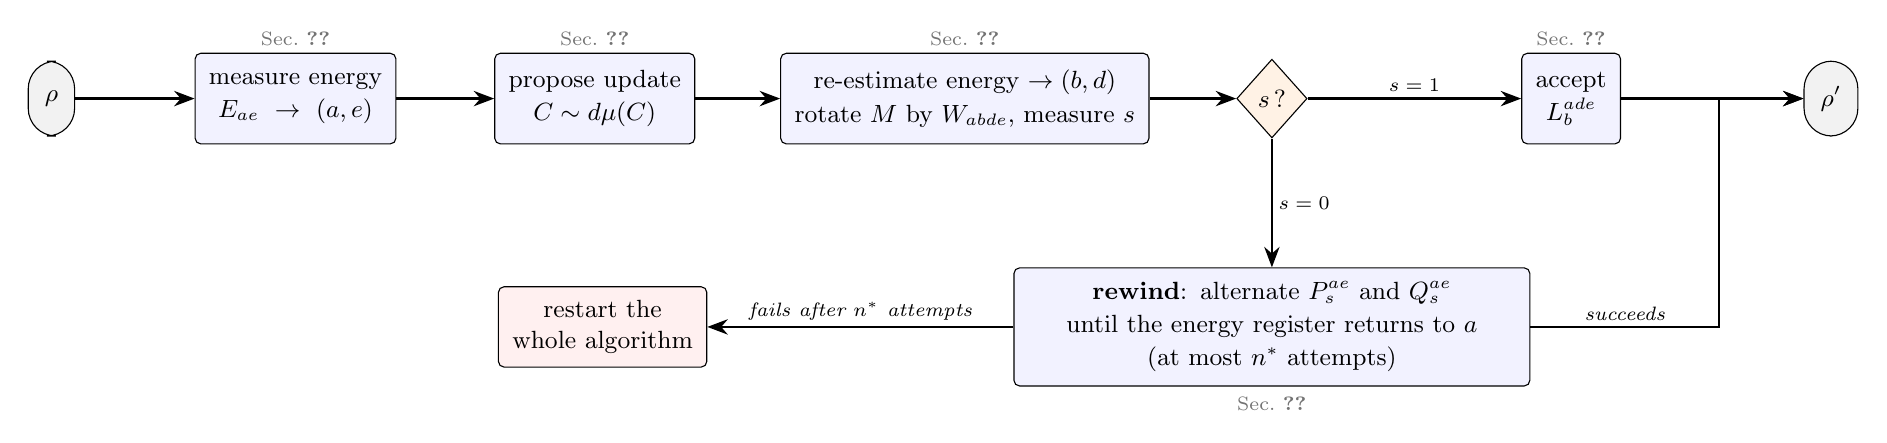
\begin{tikzpicture}[
  font=\small,
  box/.style   = {draw, rounded corners=2pt, align=center, minimum height=1.15cm, inner sep=5pt, fill=blue!5},
  dec/.style   = {draw, diamond, aspect=1.6, align=center, inner sep=1pt, fill=orange!10, minimum height=1.0cm},
  term/.style  = {draw, rounded corners=10pt, align=center, minimum height=0.95cm, inner sep=6pt, fill=black!5},
  fail/.style  = {draw, rounded corners=2pt, align=center, minimum height=0.95cm, inner sep=5pt, fill=red!6},
  ar/.style    = {-{Stealth[length=2.6mm]}, thick},
  lbl/.style   = {font=\scriptsize\itshape, inner sep=2pt, fill=white},
  sec/.style   = {font=\scriptsize, text=black!55, inner sep=1.5pt}
]
\node[term] (rin)  at (0,0)    {$\rho$};
\node[box]  (E)    at (3.1,0)  {measure energy\\[1pt] $E_{ae}\ \rightarrow\ (a,e)$};
\node[box]  (C)    at (6.9,0)  {propose update\\[1pt] $C\sim d\mu(C)$};
\node[box]  (W)    at (11.6,0) {re-estimate energy $\rightarrow (b,d)$\\[1pt] rotate $M$ by $W_{abde}$, measure $s$};
\node[dec]  (D)    at (15.5,0) {$s\,$?};
\node[box]  (A)    at (19.3,0) {accept\\[1pt] $L^{ade}_b$};
\node[term] (rout) at (22.6,0) {$\rho'$};
\node[box, text width=6.2cm] (R) at (15.5,-2.9)
      {\textbf{rewind}: alternate $P^{ae}_s$ and $Q^{ae}_s$\\[1pt]
       until the energy register returns to $a$\\[1pt] (at most $n^*$ attempts)};
\node[fail] (F) at (7.0,-2.9)  {restart the\\ whole algorithm};

\node[sec, above=1pt of E] {Sec.~\ref{section:energymeasurement}};
\node[sec, above=1pt of C] {Sec.~\ref{section:update}};
\node[sec, above=1pt of W] {Sec.~\ref{section:acceptprob}};
\node[sec, above=1pt of A] {Sec.~\ref{section:acceptprob}};
\node[sec, below=2pt of R] {Sec.~\ref{section:rejection}};

\draw[ar] (rin) -- (E);
\draw[ar] (E)   -- (C);
\draw[ar] (C)   -- (W);
\draw[ar] (W)   -- (D);
\draw[ar] (D)   -- node[lbl,above]{$s=1$} (A);
\draw[ar] (A)   -- (rout);
\draw[ar] (D)   -- node[lbl,right]{$s=0$} (R);
\draw[ar] (R.east) -- node[lbl,above]{succeeds} ++(2.4,0) |- (rout.west);
\draw[ar] (R.west) -- node[lbl,above]{fails after $n^*$ attempts} (F.east);
\end{tikzpicture}}
\caption{One complete round of the algorithm. The state is measured in energy, an update $C$ is proposed and applied, and the energy is estimated again; a single-qubit rotation whose angle depends on the two energy readouts decides acceptance. On rejection the state cannot simply be copied back, so it is driven back to its original energy by an alternating sequence of two projective measurements (the ``rewind'' loop of Section~\ref{section:rejection}); this succeeds with probability at least $1-\frac{1}{2n^*}$. Every stage reuses the \emph{same} persistent registers $R$ (energy readout), $F$ (direction bit) and $M$ (acceptance rotation), defined in Table~\ref{tab:notation}, which is precisely why the phase estimation must be state independent.}
\label{fig:overview}
\end{figure*}

\begin{table*}
\caption{Notation used throughout. Modular arithmetic is understood on the energy register: $|x|_N = \min(x \bmod N, -x \bmod N)$.}
\label{tab:notation}
\begin{ruledtabular}
\footnotesize
\begin{tabular}{ll@{\quad}ll}
\multicolumn{2}{c}{\textbf{Registers, states and operators}} & \multicolumn{2}{c}{\textbf{Parameters}}\\[2pt]
$H$, $\ket{\psi_j}$, $E_j$ & Hamiltonian on $m$ qubits and its eigenpairs & $\eta$ & ancilla qubits in $R$; the register holds $2^{\eta}$ values\\
$\sigma_G$, $\sigma^*$ & Gibbs state; actual fixed point of one round & $t=\frac{1}{16\|H\|}$ & evolution time inside BSI-QPE\\
$R$ & persistent $\eta$-qubit energy-readout register & $\beta$ & inverse temperature (bare $\beta$, no argument)\\
$F$ & persistent direction qubit acted on by $G^{pq}_j$ & $\mu$ & truncation bandwidth, in energy bins\\
$M$ & persistent qubit carrying the acceptance rotation & $\nu=\frac13\sin^2\frac{\pi}{4b}$ & Fourier decay rate of the windows\\
$\Omega_{RFM}$ & initial state $\ket{0}_R\otimes\frac{\mathbb I_F}{2}\otimes\ket{0}_M$ & $b$, $r$ & window shape parameters (Appendix~\ref{section:appendix})\\
$C$, $d\mu(C)$ & proposed update and its distribution & $n^*$ & cap on rewinding attempts\\
$G^{pq}_j$, $\tilde G^{pq}_j$ & $2\times2$ block of BSI-QPE; band-limited version & $c=\log\mu$ & extra ancilla qubits, Eq.~\eqref{eq:headline}\\
$W_{abde}$, $f_{abde}$ & acceptance rotation on $M$ and its probability & &\\[4pt]
\multicolumn{2}{c}{\textbf{Indices}} & \multicolumn{2}{c}{\textbf{Error symbols}}\\[2pt]
$a$, $e$ & energy value and direction bit read \emph{before} the update & $\epsilon_{\Delta}$ & window mass outside the band, $O(\sqrt{2^{\eta}}e^{-\nu\mu})$\\
$b$, $d$ & energy value and direction bit read \emph{after} the update & $\epsilon_m$ & multiplicative error in Lemma~\ref{lemma:1}\\
$s\in\{0,1\}$ & accept flag; $s=1$ accepts & $\epsilon_a$ & additive (truncation) error\\
$j,k,l,m$ & eigenstate labels & $\epsilon_{\mathcal A},\epsilon_{\mathcal B}$ & reweighting errors for $\mathcal A$ and $\mathcal B(n)$\\
$p,q$ & register indices summed inside $G^{pq}_j$ & $\epsilon_c$ & total per-round error, Eq.~\eqref{eq:error_bound}\\
$\lambda$ & label of a $2$D invariant subspace (Sec.~\ref{section:rejection}) & $\epsilon^T_t$ & operator-norm error of the time evolution\\
$n$ & number of completed rewind iterations & $\kappa_{abde}$ & unwrapped energy difference, Eq.~\eqref{eq:kappadef}\\
\end{tabular}
\end{ruledtabular}
\vspace{2pt}
\footnotesize\noindent\emph{Symbols carrying more than one meaning.} A few collisions are unavoidable given standard usage in the two literatures this paper draws on; in each case the context disambiguates.
$\beta$ \emph{with} an argument, $\beta(x)$ or $\hat\beta(k)$, is the second window function; \emph{bare} $\beta$ is the inverse temperature.
$k$ is the value stored in $R$ when it appears as a summation index in Section~\ref{section:boostedphaseestimation}, an eigenstate label in $\ket{\psi_k}$, the integer multiple of $2^{\eta}$ removed by the unwrapping in Eq.~\eqref{eq:kappadef}, and the contraction factor in Theorem~\ref{theorem:error_bound}.
$m$ is the number of system qubits in Section~\ref{section:boostedphaseestimation} and an eigenstate label thereafter.
$p$ is a register index, whereas $p^{ae\lambda}$ in Section~\ref{section:rejection} is an acceptance probability.
Finally, the decay rate $\nu$ and the reweighting factor $v^j_m$ of Section~\ref{section:rejectionbranch} are distinct symbols.
\end{table*}

\section{Boosted State-Independent Quantum Phase Estimation}
\label{section:boostedphaseestimation}
Given an $m$-qubit Hamiltonian $H$ with eigenvectors $\ket{\psi_j}$ such that $H\ket{\psi_j} = E_j \ket{\psi_j}$, quantum phase estimation (QPE) allows one to prepare an ancilla register that approximates $E_j$. Unfortunately, quantum computers have limited precision. As a result, unless the energy can be represented exactly in binary using $\eta$ bits (corresponding to $\eta$ ancilla qubits), there is a high probability of obtaining an inaccurate energy measurement. This inaccuracy arises from the ``fat tails" in QPE \cite{Nielsen_Chuang_2010}.

It is convenient to name the three registers now, since all of them persist through an entire round of the algorithm (Fig.~\ref{fig:overview}). $R$ is the $\eta$-qubit register that holds the energy readout; $F$ is a single additional qubit recording the \emph{direction} in which $R$ has been shifted; and $M$ is a further single qubit, introduced in Section~\ref{section:acceptprob}, which carries the acceptance rotation and is reused by every acceptance test thereafter. BSI-QPE acts on the system register together with $R$ and $F$; it does not touch $M$.

Often this issue can be mitigated by simply repeating the calculation and taking an average. However, Quantum Metropolis sampling requires us to ``rewind" upon rejecting a proposed update and hence we require a unitary method for ``boosting" QPE. This ``boosted" QPE stores an approximation to the energy in ancillas which is not immediately measured but rather used as the basis for further coherent calculations. Further, for ``rewinding" to work we must reuse the same ancilla registers so the QPE protocol must also be state-independent. Therefore, we must demonstrate an implementation of a boosted state-independent quantum phase estimation (BSI-QPE). While it has been shown \cite{chen2023quantumthermalstatepreparation} that QPE cannot entirely eliminate the probability mass in its tails, we demonstrate that it is possible to construct BSI-QPE protocols with exponentially suppressed tails, which effectively mitigate the issue for practical purposes. 

Existing methods for boosting QPE rely upon choosing specific input ancillary states. In these methods QPE is performed using ancillas initialised to the state $\sum_x \alpha(x) \ket{x}$ for some window function $\alpha(x)$ instead of the standard uniform superposition. After performing QPE upon eigenstate $\ket{\psi_j}$ the following state is produced:
\begin{equation}
   \frac{1}{\sqrt{2^{\eta}}} \sum_x \sum_k e^{\frac{2 \pi i}{2^{\eta}}x(k-E_j)} \alpha(x)\ket{k}\ket{\psi_j}
\end{equation}
which can be rewritten as:
\begin{equation}
    \sum_k \hat\alpha(k-E_j) \ket{k}\ket{\psi_j}
\end{equation}
where $\hat \alpha(k)$ is the discrete Fourier transform of $\alpha(x)$. By choosing $\alpha$ to be a window function one can ensure that $\hat \alpha$ is narrowly peaked, thus QPE is boosted. Unfortunately, this is not sufficient for the quantum Metropolis algorithm as we require the QPE to be independent of the ancillary state, as we must reuse the same ancillas throughout the rewinding process. 

Our construction uses two window functions $\alpha(x)$ and $\beta(x) = \sqrt{1-\alpha(x)^2}$ (for $x\in\{0,1,\ldots,2^{\eta}-1\}$) which are both narrowly peaked in the Fourier domain. We introduce these windows via the following multi-controlled single-qubit rotation:
\begin{equation}
   CR_Y = \sum_k \ket{k}\bra{k}\otimes \begin{pmatrix}
        \alpha(k)& \beta(k)\\
        -\beta(k)& \alpha(k)
    \end{pmatrix}
\end{equation}

We also require the following time evolution gadget which is constructed as shown in Fig~\ref{fig:CRZ}:
\begin{equation}
    CR_Z =\sum_{j,k}\ket{\psi_j}\bra{\psi_j}\otimes\ket{k}\bra{k} \otimes \begin{pmatrix}
        e^{\frac{iE_jkt}{2}}&0\\
        0 & e^{-\frac{iE_jkt}{2}}
    \end{pmatrix}
\end{equation}
\begin{figure*}
\[
\vcenter{\hbox{
\resizebox{!}{2.5cm}{
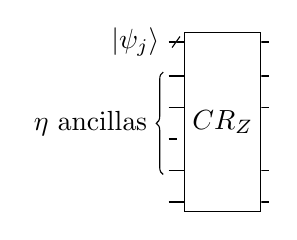
\begin{tikzpicture}
\begin{yquant*}
qubit {$\ket{\psi_j}$} s;

init {$\eta$ ancillas} (a[0,1],ellipsis, aend);
slash s;
hspace {0.1cm} -;
discard ellipsis;
% qubit {} aend;
qubit {} f;
box {$CR_Z$} (s,a,ellipsis, aend, f);

% text {$\ket{0}$} f;
\end{yquant*}
\end{tikzpicture}}}}
=
\vcenter{\hbox{
\resizebox{!}{2.5cm}{
    \begin{tikzpicture}
\begin{yquant*}
qubit {$\ket{\psi_j}$} s;

init {$\eta$ ancillas} (a[0,1],ellipsis, aend);
discard ellipsis;
% qubit {} aend;
qubit {} f;
slash s;
hspace {0.1cm} -;

box {$U^{\dagger 2^0}$} (s) | a[0], f;
box {$U^{\dagger 2^1}$} (s) | a[1], f;
hspace {0mm} -;
dots ellipsis;

box {$U^{\dagger 2^{\eta-1}}$} (s) | aend[0], f;
box {$U^{2^0}$} (s) | a[0]~ f;
box {$U^{ 2^1}$} (s) | a[1]~ f;
hspace {0mm} -;
dots ellipsis;

box {$U^{ 2^{\eta-1}}$} (s) | aend[0]~ f;
\end{yquant*}
\end{tikzpicture}}}}
\]
\caption{Quantum circuit for implementing an $Z$ rotation on an ancilla qubit that is dependent upon the energy of the system. The unitary $U=e^{\frac{iHt}{2}}$ is implemented through some quantum time evolution algorithm (e.g. trotterisation \cite{lloyd1996universal}, qubitization \cite{Low2019hamiltonian}) up to an operator norm error of $\epsilon^T_t$. Throughout this work we assume  $\epsilon^T_t$ is negligible, and use perfect quantum time evolution in our error analysis.}
    \label{fig:CRZ}
\end{figure*}
Both of these act as controlled $R_Z$ and $R_Y$ rotations on a single qubit. 
\begin{figure*}
\[
\vcenter{\hbox{
\resizebox{!}{2.5cm}{
\begin{tikzpicture}
    \begin{yquant*}
qubit {$\ket{\psi_j}$} s;

init {$\eta$ ancillas} (a[0,1],ellipsis, aend);
slash s;
% hspace {0.1cm} -;
discard ellipsis;
% qubit {} aend;
qubit {} f;
dots ellipsis;

box {BSI-\\QPE} (s,a,ellipsis, aend, f);

% text {$\ket{0}$} f;
\end{yquant*}
\end{tikzpicture} }}}
=
\vcenter{\hbox{
\resizebox{!}{2.5cm}{
\begin{tikzpicture}
    \begin{yquant*}
qubit {$\ket{\psi_j}$} s;

init {$\eta$ ancillas} (a[0,1],ellipsis, aend);
slash s;
discard ellipsis;
% qubit {} aend;
qubit {} f;
dots ellipsis;
box {QFT} (a,ellipsis, aend);

[this subcircuit box style={dashed, "$R_Z[E_jt(k-k')]$"}]
subcircuit {
qubit {} s;
qubit {} a[2];
nobit ellipsis;
qubit {} aend;
qubit {} f;

% dots ellipsis;
box {$CR_Z$} (s,a,ellipsis, aend, f);

x aend[0];
dots ellipsis;
box {$CR_Z^{\dagger}$} (s,a,ellipsis, aend, f);
x aend[0];
dots ellipsis;
} (s,a,ellipsis, aend, f);

box {$CR_Y$} (a,ellipsis, aend, f);

[this subcircuit box style={dashed, "$R_Z[E_jt(k+k'-2^{\eta})]$"}]
subcircuit {
qubit {} s;
qubit {} a[2];
nobit ellipsis;
qubit {} aend;
qubit {} f;

box {$CR_Z$} (s,a,ellipsis, aend, f);
x aend[0];
dots ellipsis;
box {$CR_Z$} (s,a,ellipsis, aend, f);
x aend[0];
dots ellipsis;
box {$U^{\dagger 2^{\eta}}$} (s) ~ f;
box {$U^{2^{\eta}}$} (s) | f;
} (s,a,ellipsis, aend, f);

box {iQFT} (a,ellipsis, aend);

% text {$\ket{0}$} f;
\end{yquant*}
\end{tikzpicture} }}}
\]

\caption{Quantum circuit implementing boosted state-independent quantum phase estimation (BSI-QPE). We highlight how the combinations of $CR_Z$ and $X$ gates operators correspond to the single qubit $R_Z$ given in Eq.~\ref{eq:euler} with $k$ being the value stored in the $\eta$ ancillas and $k' = k + 2^{\eta-1} \mod 2^{\eta}$}
\label{fig:circuit}
\end{figure*}
\begin{figure*}
\begin{tikzpicture}
    \begin{yquant*}
qubit {$\ket{\psi_j}$} s;

init {$\eta$ ancillas} (a[0,1],ellipsis, aend);
slash s;
discard ellipsis;
% qubit {} aend;
dots ellipsis;
box {QFT} (a,ellipsis, aend);

box {$U^{ 2^1}$} (s) | a[0];
box {$U^{ 2^2}$} (s) | a[1];
hspace {0mm} -;
dots ellipsis;

box {$U^{ 2^{\eta}}$} (s) | aend[0];
box {$U^{\dagger 2^{\eta}}$} (s);
box {iQFT} (a,ellipsis, aend);

% text {$\ket{0}$} f;
\end{yquant*}
\end{tikzpicture} 

\caption{Quantum circuit implementing unboosted state-independent QPE with $U=e^{\frac{iHt}{2}}$, equivalent to choosing $\alpha(x)=1$ for BSI-QPE and acting upon $\ket{0}_F$. This slightly differs from the standard formulation of QPE \cite{Nielsen_Chuang_2010} by beginning with $QFT$ rather than $H^{\otimes \eta}$ and the addition of $U^{\dagger 2^{\eta}}$ at the end. }
\label{fig:standard_qpe}
\end{figure*}

\begin{widetext}
We can implement BSI-QPE through the circuit illustrated in Fig~\ref{fig:circuit}. This circuit combines the  $CR_Z$ and $CR_Y$ rotations using the following $R_ZR_YR_Z$ decomposition \cite{Nielsen_Chuang_2010}: 
\begin{equation}
\label{eq:euler}
    R_Z[E_jt(k+k'-2^{\eta})]R_Y[2\arccos(\alpha(k))]R_Z[E_jt(k-k')] = \begin{pmatrix}
        \alpha(k)e^{iE_jtk}e^{-iE_jt2^{\eta-1}} && \beta(k)e^{iE_jt k'}e^{-iE_jt2^{\eta-1}}\\
        -\beta (k)e^{-iE_jt k'}e^{iE_jt2^{\eta-1}} && \alpha(k)e^{-iE_jtk}e^{iE_jt2^{\eta-1}}
    \end{pmatrix}
\end{equation}
In Fig.~\ref{fig:circuit}, the $X$-gates acting on the last qubit in the ancilla register shift the value stored from $k$ to $k'= k+2^{\eta-1} \mod 2^{\eta}$, and hence we get the following operation:
\begin{multline}
        \text{BSI-QPE} = \frac{1}{2^{\eta}}\sum_j\sum_{p,q,k} \begin{pmatrix}
        \alpha(k)e^{iE_jtk}e^{-iE_jt2^{\eta-1}} && \beta(k)e^{iE_jt[(k+2^{\eta-1})\text{mod} 2^{\eta}]}e^{-iE_jt2^{\eta-1}}\\
        -\beta (k)e^{-iE_jt[(k+2^{\eta-1})\text{mod} 2^{\eta}]}e^{iE_jt2^{\eta-1}} && \alpha(k)e^{-iE_jtk}e^{iE_jt2^{\eta-1}}
    \end{pmatrix}e^{\frac{2\pi i}{2^{\eta}}k(q-p)} \\\otimes\ket{p}\bra{q}\otimes\ket{\psi_j}\bra{\psi_j}
\end{multline}
The sum over $k$ is now a discrete Fourier transform. Pairing $e^{\frac{2\pi i}{2^{\eta}}k(q-p)}$ with $\alpha(k)e^{\pm iE_jtk}$ collapses each diagonal entry to a single transform evaluated at $q-p\pm\frac{2^{\eta}}{2\pi}E_jt$, and the modular shift $k \mapsto k+2^{\eta-1}$ appearing in the off-diagonal entries is exactly the half-grid offset absorbed into the definition of $\hat\alpha$ in Eq.~\eqref{eq:alphahat} below. This gives:
\begin{equation}
    \text{BSI-QPE} = \frac{1}{\sqrt{2^{\eta}}}\sum_j\sum_{p,q} \begin{pmatrix}
        (-1)^{q-p}\hat\alpha(q-p+\frac{2^{\eta}}{2\pi}E_jt) && \hat\beta(q-p+\frac{2^{\eta}}{2\pi}E_jt)\\
        -\hat\beta (q-p-\frac{2^{\eta}}{2\pi}E_jt) && (-1)^{q-p}\hat\alpha(q-p-\frac{2^{\eta}}{2\pi}E_jt)
    \end{pmatrix}\otimes\ket{p}\bra{q}\otimes\ket{\psi_j}\bra{\psi_j}
\end{equation}
% \begin{multline}
%   \sum_j \sum^{2^{\eta}}_{p,q} \hat \alpha(p - q - \frac{2^{\eta} t}{2\pi}E_j)\ket{0}\bra{0} \otimes\ket{p}\bra{q} \otimes \ket{\psi_j} \bra{\psi_j}\\
%   + \ket{0}\bra{0} \otimes\bm{\varepsilon}^T_{kt}
% \end{multline}
where $\hat \alpha$ is the discrete Fourier transform of $\alpha$ as given by:
\begin{equation}
   \hat\alpha(x) =\frac{1}{\sqrt{2^{\eta}}}\sum_{k=-2^{\eta-1}}^{2^{\eta-1}-1} \alpha(k+2^{\eta-1})e^{\frac{2\pi i}{2^{\eta}}xk}
   \label{eq:alphahat}
\end{equation}
and $\hat \beta$ is the discrete Fourier transform of $\beta$ given by:
\begin{equation}
    \hat\beta(x) =\frac{1}{\sqrt{2^{\eta}}}\sum_{k=-2^{\eta-1}}^{2^{\eta-1}-1} \beta(k)e^{\frac{2\pi i}{2^{\eta}}kx}
\end{equation}
 where $\beta(k)$ is extended by $\beta(k) = \beta(k \mod 2^{\eta})$. We have defined $\hat \alpha$ as the discrete Fourier transform of $\alpha(k)$ shifted by $2^{\eta-1}$. This is essential as $|\alpha|^2+|\beta|^2=1$, so without this shift we cannot have both $\alpha, \beta \ll1$ at the boundary of the discrete Fourier transform and hence we would observe spectral leakage (for non-integer $k$) that precludes exponentially decaying tails. Throughout the rest of this work, we will use the following notational shorthand: 
\begin{equation}
    G_j^{pq} = \begin{pmatrix}
        (-1)^{q-p}\hat\alpha(q-p+\frac{2^{\eta}}{2\pi}E_jt) && \hat\beta(q-p+\frac{2^{\eta}}{2\pi}E_jt)\\
        -\hat\beta (q-p-\frac{2^{\eta}}{2\pi}E_jt) && (-1)^{q-p}\hat\alpha(q-p-\frac{2^{\eta}}{2\pi}E_jt)
    \end{pmatrix}
\end{equation}
This shows that BSI-QPE shifts the energy-index register by approximately $\frac{2^{\eta}}{2\pi}E_jt$, in a direction given by the qubit $F$ after the application. Figure~\ref{fig:twopeaks} illustrates what this means for the amplitudes: acting on an energy eigenstate, BSI-QPE does not produce one peak, but two --- one shifted to $+\frac{2^{\eta}}{2\pi}E_jt$ and one to $-\frac{2^{\eta}}{2\pi}E_jt$ --- and which of the two a given branch sits in is recorded by $F$. Reading $F$ together with $R$ therefore recovers the signed energy $(-1)^e a$. The whole point of the window construction is that each of these two peaks has tails that fall off exponentially rather than as $1/k$.
\end{widetext}

\begin{figure}[t]
\centering
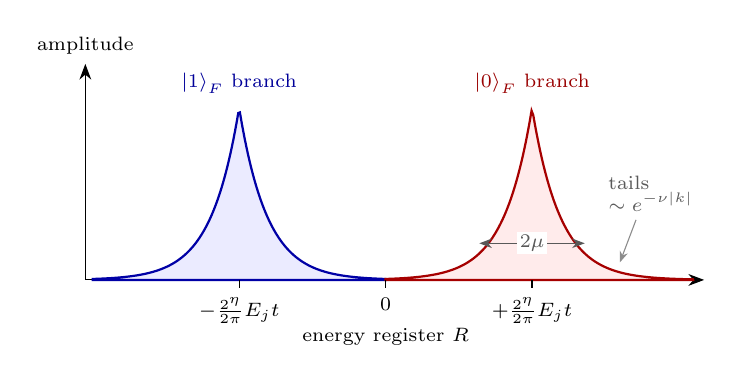
\begin{tikzpicture}[font=\small,scale=0.93]
\def\D{2.0}
\def\hgt{2.35}
\def\rate{2.6}
% axis
\draw[-{Stealth[length=2mm]}] (-4.1,0) -- (4.35,0);
\node[font=\scriptsize] at (0,-0.78) {energy register $R$};
\draw[-{Stealth[length=2mm]}] (-4.1,0) -- (-4.1,2.95) node[above,font=\scriptsize,align=center] {amplitude};
% peaks
\draw[thick,blue!65!black,fill=blue!12,fill opacity=0.65]
   plot[domain=-4.0:0.0,samples=180] (\x,{\hgt*exp(-\rate*abs(\x+\D))}) -- (0,0) -- (-4.0,0) -- cycle;
\draw[thick,red!65!black,fill=red!12,fill opacity=0.65]
   plot[domain=0.0:4.2,samples=180] (\x,{\hgt*exp(-\rate*abs(\x-\D))}) -- (4.2,0) -- (0,0) -- cycle;
% ticks
\foreach \x/\lab in {-\D/{$-\frac{2^{\eta}}{2\pi}E_jt$}, 0/{$0$}, \D/{$+\frac{2^{\eta}}{2\pi}E_jt$}}
  \draw (\x,0) -- (\x,-0.11) node[below,font=\scriptsize] {\lab};
% branch labels
\node[blue!60!black,font=\scriptsize,align=center] at (-2.0,\hgt+0.34) {$\ket{1}_F$ branch};
\node[red!60!black,font=\scriptsize,align=center]  at ( 2.0,\hgt+0.34) {$\ket{0}_F$ branch};
% bandwidth bracket
\draw[{Stealth[length=1.6mm]}-{Stealth[length=1.6mm]}, black!65]
   (\D-0.72,0.50) -- (\D+0.72,0.50) node[midway,fill=white,inner sep=1pt,font=\scriptsize] {$2\mu$};
% tail annotation
\node[font=\scriptsize,black!65,align=left] at (3.62,1.18) {tails\\ $\sim e^{-\nu|k|}$};
\draw[black!45,-{Stealth[length=1.4mm]}] (3.42,0.82) -- (3.20,0.24);
\end{tikzpicture}
\caption{What BSI-QPE does to the energy register, for a single eigenstate $\ket{\psi_j}$. Two peaks are produced, displaced by $\pm\frac{2^{\eta}}{2\pi}E_jt$, and the direction qubit $F$ labels which one a branch belongs to. Truncating each peak to the $2\mu$ bins around its centre (Lemma~\ref{lemma:0}) discards only the shaded tails; because the windows of Appendix~\ref{section:appendix} decay as $e^{-\nu|k|}$, that discarded mass is $\epsilon_{\Delta}=O(\sqrt{2^{\eta}}e^{-\nu\mu})$. With an unboosted (rectangular) window the tails would instead fall off only as $1/k$, and no useful truncation would be possible --- this is the content of Remark~\ref{remark:boosting}.}
\label{fig:twopeaks}
\end{figure}
There are many potential candidates for window functions $\alpha(x)$ and $\beta(x)$. In this work we choose to work with $\alpha(x) = \text{sech}( r\cos^{2b} \frac{\pi x}{2^{\eta}})$ and $\beta(x) = \text{tanh}(r \cos^{2b} \frac{\pi x}{2^{\eta}})$. These can both be shown to have discrete Fourier transforms which decay exponentially fast as we discuss in Appendix~\ref{section:appendix}:
\begin{equation}
    |\hat \alpha(k)|,|\hat \beta(k)| = O\left( \sqrt{2^{\eta}}e^{-\nu |k|}\right)
    \label{eq:scaling}
\end{equation}
where $\nu = \frac{1}{3}\sin^2\frac{\pi}{4b}$. Hence we can write:
\begin{equation}
    \hat\alpha(k) = \tilde\alpha(k) + \Delta_{\alpha}(k) \>\>\>\>\>\>\hat\beta(k) = \tilde\beta(k) + \Delta_{\beta}(k)
    \label{eq:decomposealpha}
\end{equation}
where:
\begin{align}
    \tilde\alpha(k) &= \hat\alpha(k)\mathbbm{1}(|k|_{2^{\eta}}\leq \mu)\\
    \tilde\beta(k) &= \hat\beta(k)\mathbbm{1}(|k|_{2^{\eta}}\leq \mu)
    \label{eq:decomposealpha2}
\end{align}  and
\begin{equation}
    \sum_k|\Delta_\alpha(k)|,\sum_k|\Delta_\beta(k)|\leq \epsilon_{\Delta}
    \label{eq:decomposealpha3}
\end{equation} where $\epsilon_{\Delta} = O(\sqrt{2^{\eta}}e^{-\nu \mu})$ and $|x|_N = \min(x \mod N,- x\mod N)$ is the modular norm value of $x$.

\begin{lemma}[Band-limited BSI-QPE]
\label{lemma:0}
    Define $\widetilde{\text{BSI-QPE}}$ as given by:
    \begin{equation}
       \widetilde{\text{BSI-QPE}}= \frac{1}{\sqrt{2^{\eta}}}\sum_j \sum_{p,q} \tilde G^{pq}_j \otimes \ket{p}\bra{q} \otimes \ket{\psi_j}\bra{\psi_j}
    \end{equation}
    where 
    \begin{equation}
        \tilde G^{pq}_j = \begin{pmatrix}
        (-1)^{q-p}\tilde\alpha(q-p+\frac{2^{\eta}}{2\pi}E_jt) && \tilde\beta(q-p+\frac{2^{\eta}}{2\pi}E_jt)\\
        -\tilde\beta (q-p-\frac{2^{\eta}}{2\pi}E_jt) && (-1)^{q-p}\tilde\alpha(q-p-\frac{2^{\eta}}{2\pi}E_jt)
    \end{pmatrix}
    \end{equation}
    Then,  
    \begin{equation}
        \|\widetilde{\text{BSI-QPE}}-\text{BSI-QPE}\| \leq \frac{2\epsilon_{\Delta}}{\sqrt{2^{\eta}}}
    \end{equation}
\end{lemma}
Proof is given in Appendix~\ref{section:appendixTrunc}. This shows that our BSI-QPE protocol is very close in operator norm to a fully band-limited BSI-QPE.

\begin{remark}[Why boosting is necessary]
\label{remark:boosting}
Instead one could attempt to use unboosted state-independent QPE. This would correspond to choosing $\alpha(x)=1$, which simplifies Fig.~\ref{fig:circuit} to Fig.~\ref{fig:standard_qpe}. As this effectively acts as a rectangular window function, $|\hat\alpha(k)| = O(\frac{\sqrt{2^{\eta}}}{k})$ for off-grid $k$, so $\epsilon_{\Delta} = O(\sqrt{2^{\eta}}\log \frac{2^\eta}{\mu})$. This bound exceeds $\sqrt{2^{\eta}}$ and so unboosted state-independent QPE is insufficient for Quantum Metropolis sampling without the promise of energies exactly represented in $\eta$ bits.
\end{remark}
\section{Algorithm}
\label{section:algorithm}
Quantum Metropolis is heavily inspired by the classical Metropolis--Hastings algorithm. The principal idea is to apply a randomly chosen update to the current state then accept/reject this update with a probability given by a function ($\tilde{f}_{E_aE_b}=\min(1, e^{-\beta(E_b-E_a)})$) of the energy before $(E_a)$ and after $(E_b)$ the update. This update process is repeated many times with the system quickly converging to equilibrium. To replicate this on a quantum computer we need to be able to: measure the energy of a state (Section~\ref{section:energymeasurement}), apply some update (Section~\ref{section:update}), accept/reject an update with the correct probability (Section~\ref{section:acceptprob}) and ``undo" an update upon deciding to reject it (Section~\ref{section:rejection}).
Figure~\ref{fig:overview} shows the whole round; this section fills in each box in turn.

Before doing so we fix the index conventions, because four letters carry most of the notation from here to the end of the paper. \emph{Every subsequent equation in Sections~\ref{section:algorithm} and~\ref{section:why} should be read with the following in mind:}
\begin{quote}
$(a,e)$ are the energy-register value and direction bit produced by BSI-QPE \textbf{before} the update; $(b,d)$ are the corresponding pair produced \textbf{after} it; $s\in\{0,1\}$ is the accept flag, with $s=1$ meaning accept; and $\kappa_{abde}$, defined in Eq.~\eqref{eq:kappadef}, is the unwrapped energy difference these four readouts encode, on which the acceptance probability $f_{abde}$ depends.
\end{quote}
The four measurements built in this section then have simple readings, collected in Table~\ref{tab:operators}; it is worth keeping that table to hand while reading Section~\ref{section:why}, where the same four symbols appear throughout.

\begin{table}[b]
\caption{The four measurements making up one round, and the question each one asks. All four act on the \emph{same} persistent registers.}
\label{tab:operators}
\begin{ruledtabular}
\begin{tabular}{lll}
Operator & Plain reading & Defined in \\
\hline
$E_{ae}$ & what is the energy of the current state? & Sec.~\ref{section:energymeasurement}\\
$Q^{ae}_s$ & did the accept/reject rotation succeed? & Sec.~\ref{section:acceptprob}\\
$L^{ade}_b$ & accept the update and finish the round & Sec.~\ref{section:acceptprob}\\
$P^{ae}_s$ & have we returned to the original energy? & Sec.~\ref{section:rejection}\\
\end{tabular}
\end{ruledtabular}
\end{table}

Throughout one full update, let $R$ denote the $\eta$-qubit BSI-QPE energy-index register and qubit $F$ the additional qubit on which the $G_j^{pq}$ act. At the start of the update, $R$ is initialised to $\ket{0}$ whilst $F$ is in the maximally mixed state (by classically randomly choosing initial state $\ket{0}$ or $\ket{1}$) and the qubit $M$ on which the acceptance rotation $W_{abde}$ acts is initialized in $\ket{0}$. The same register $R$ and $F$ are used by $E_{ae}$ and by every subsequent $P_s^{ae}$ and $Q_s^{ae}$ measurement; it is never reset during the update. Likewise, $M$ is reused by every $Q_s^{ae}$ and is left untouched by $P_s^{ae}$. Fresh pointer qubits may be used to record measurement outcomes and are not part of the persistent work register. This reuse is not an optimisation: it is the reason the phase estimation of Section~\ref{section:boostedphaseestimation} has to be state independent, since the register handed to the second and every later invocation is whatever the previous one left behind.
\subsection{Measure the energy}
\label{section:energymeasurement}
To measure the energy we use the boosted state-independent quantum phase estimation protocol set out in Section~\ref{section:boostedphaseestimation}. We simply apply BSI-QPE, measure the ancilla qubits and then apply inverse BSI-QPE, as shown in Fig.~\ref{fig:Ecircuit} and outlined below:
\begin{multline}
    E_{ae} = \frac{1}{2^{\eta}}\sum_j\sum_{p_1,p_2,p_3,p_4} \ket{\psi_j}\bra{\psi_j} \otimes \ket{p_4}\braket{p_3|a}\braket{a|p_2}\bra{p_1} \otimes \\G_j^{p_3p_4 \dagger}\ket{e}\bra{e}G_j^{p_2p_1}
\end{multline}
\begin{multline}
        E_{ae} = \frac{1}{2^{\eta}}\sum_j\sum_{p_1,p_4} \ket{\psi_j}\bra{\psi_j}\otimes\ket{p_4}\bra{p_1}\otimes\\
        G_j^{ap_4 \dagger}\ket{e}\bra{e}G_j^{ap_1}
\end{multline}
\begin{figure}
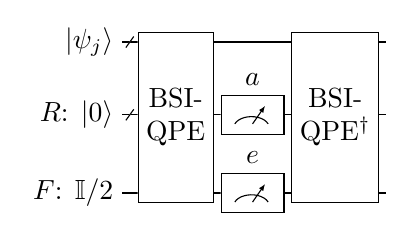
\begin{tikzpicture}
\begin{yquant*}
% init {$\eta$ ancillas} (a);
qubit {$\ket{\psi_j}$} system;
qubit {$R$: $\ket{0}$} a;
qubit {$F$: $\mathbb{I}/2$} f;

slash system;
slash a;
hspace {0.1cm} -;

box {BSI-\\QPE} (a,system,f);

["$a$",type=qubit]
measure a;

["$e$",type=qubit]
measure f;

box {BSI-\\QPE$^{\dagger}$} (a,system,f);
\end{yquant*}
\end{tikzpicture}

\caption{Quantum circuit for implementing projective measurement $E_{ae}$.}
\label{fig:Ecircuit}
\end{figure}
This measurement gives us $(-1)^ea$, which approximates the energy of the initial state. Because $E_{ae}$ is implemented as a projective measurement, its inverse BSI-QPE does not in general disentangle the work register. The post-measurement registers $R, F$ are retained and reused in all subsequent $P_s^{ae}$ and $Q_s^{ae}$ measurements in the same update.
\subsection{Update}
\label{section:update}
After measuring the initial energy we must apply an update to our state. In Quantum Metropolis this update comes in the form of a unitary operator $C$ chosen from some set $\mathcal{C}$ according to some probability measure $d\mu(C)$. It is essential for the purposes of detailed balance that the probability of choosing $C \in \mathcal{C}$ is equal to the probability of choosing $C^{\dagger} \in \mathcal{C}$ (which is alternatively expressed as $d\mu(C) = d\mu(C^{\dagger})$).
\subsection{Accept or Reject}
\label{section:acceptprob}
After applying our unitary update $C$ we must decide whether to accept or reject this update. To ensure the probability of acceptance is approximately $\tilde{f}_{E_aE_b}$, we use a combination of phase estimation, controlled rotations and single-qubit measurement (illustrated in Fig.~\ref{fig:Qcircuit}). First we apply phase estimation to the same registers $R, F$ used by $E_{ae}$. On the joint BSI-QPE space this operation is
\begin{equation}
   \frac{1}{\sqrt{2^{\eta}}}\sum_{j,b,p}G_j^{bp}\otimes\ket{b}\bra{p}\otimes\ket{\psi_j}\bra{\psi_j}
\end{equation}
Then, using the known initial energy estimate results $a$ and $e$, we perform a $W_{abde}$ rotation on $M$, which was initialized to $\ket{0}$ at the beginning of the update, controlled by $b$ from $R$ and $d$ from $F$:
\begin{equation}
    W_{abde} = \begin{pmatrix}
        \sqrt{1 - f_{abde}} & \sqrt{f_{abde}}\\
       \sqrt{f_{abde}} & -\sqrt{1 - f_{abde}}
    \end{pmatrix}
\end{equation}
Therefore, upon measuring this ancilla qubit the probability of measuring $s=1$ is given by $f_{abde}$, which we choose to approximate $\tilde f_{E_aE_b}$. This alone is insufficient to prove that quantum Metropolis converges to a Gibbs state, but it highlights the similarity with classical Metropolis. In Section~\ref{section:why} we analyse convergence rigorously.

If we measure $s=0$ (reject), then we proceed by applying $W_{abde}^{\dagger}$ ($=W_{abde}$) again after the measurement before applying inverse phase estimation and $C^{\dagger}$, to make the whole sequence ($Q_s^{ae}$) a projective binary measurement:
\begin{equation} 
    Q_s^{ae} = \frac{1}{2^{\eta}}\sum_{j,p,q,b,d}  C^{\dagger}\ket{\psi_j}\bra{\psi_j}C \otimes \ket{q}\bra{p} \otimes G_j^{bq\dagger}\ket{d}\bra{d}G_j^{bp}\otimes R^{abde}_s
\end{equation}
where $R^{abde}_s = W_{abde}\ket{s}\bra{s}W_{abde}$. If instead we measure $s=1$ (accept) we simply measure the energy register and then apply inverse BSI-QPE. We represent this accept process as $L^{ade}_b$ as defined in Fig.~\ref{fig:LQ_circuit} and gives the following operator:
\begin{equation}
    L^{ade}_b = \frac{1}{2^{\eta}}\sum_{j,p,q}\ket{\psi_j}\bra{\psi_j}C \otimes \ket{q}\bra{p} \otimes G^{bq\dagger}_j \ket{d}\bra{d}G^{bp}_j \otimes \ket{1}\bra{1}W_{abde}
\end{equation}

The $R,F$ registers in the first $Q_s^{ae}$ measurement are the same registers used in $E_{ae}$, not separately initialized registers. Every later $P_s^{ae}$ and $Q_s^{ae}$ measurement in the update reuses these registers without resetting them. The acceptance-rotation qubit $M$ is initialized to $\ket{0}$ once and is similarly reused in every $Q_s^{ae}$. This common-register structure is shown in Fig.~\ref{fig:fullcircuit} and is required for the Marriott--Watrous rewinding argument below.
\begin{figure}
\begin{tikzpicture}
\begin{yquant*}
% init {$\eta$ ancillas} (a);
qubit {$\ket{\psi_j}$} system;
qubit {$R, F$} a;
qubit {$M:\ket{0}$} f;

slash system;
slash a;
hspace {0.1cm} -;
box {$C$} (system);
box {BSI-\\QPE} (a,system);
[multictrl]
box {$W_{abde}$} (f) ~ a;



["$s$",type=qubit]
measure f;
% text {$\ket{b}$} (a);


[multictrl]
box {$W_{abde}$} (f) ~ a;

box {BSI-\\QPE$^{\dagger}$} (a,system);
box {$C^{\dagger}$} (system);
\end{yquant*}
\end{tikzpicture}

\caption{Quantum circuit for implementing projective measurement $Q_s^{ae}$. The BSI-QPE registers $R, F$ are the same registers used by $E_{ae}$ and $P_s^{ae}$, while the rotation qubit $M$ is reused in every $Q_s^{ae}$ without being reset. It is necessary to apply $W_{abde}$ before and after the measurement to make the whole measurement projective (as $W_{abde}^{\dagger}=W_{abde}$). The slashed control denotes multiplexed control \cite{low2024trading}.}
\label{fig:Qcircuit}
\end{figure}

\begin{figure}
\begin{tikzpicture}
\begin{yquant*}
% init {$\eta$ ancillas} (a);
qubit {$\ket{\psi_j}$} system;
qubit {$R,F$} a;
qubit {$M$} f;

slash system;
slash a;
hspace {0.1cm} -;
box {$C$} (system);
box {BSI-\\QPE} (a,system);
[multictrl]
box {$W_{abde}$} (f) ~ a;



["$s=1$",type=qubit]
measure f;
["$b\>\>d$",type=qubit]
measure a;
% text {$\ket{b}\bra{b}$} (a);
box {BSI-\\QPE$^{\dagger}$} (a,system);
\end{yquant*}
\end{tikzpicture}

\caption{Quantum circuit for implementing the accept process $L_b^{ade}$. The energy register is measured after the acceptance rotation has succeeded ($s=1$), yielding the post-update readout $(b,d)$, and inverse BSI-QPE then returns the ancillas.}
\label{fig:LQ_circuit}
\end{figure}
\subsection{Rejection process}
Upon rejection in the classical algorithm we can simply revert back to an earlier copy we made of the initial state or we may be able to reverse the update applied. However, in the quantum setting the no-cloning principle rules out the former and the irreversibility of measurement rules out the latter. Therefore, we need a new technique to return to our initial state.

We use an iterative sequence of binary projective measurements similar to the QMA verification amplification of Marriott and Watrous \cite{MarriottWatrous}. The first measurement $Q_s^{ae}$ has already been introduced, whilst the second $P_s^{ae}$ simply reports whether the state has returned to the initial energy:


\begin{equation}
    P^{ae}_1 = \frac{1}{2^{\eta}}\sum_{j,p,q} \left( \ket{\psi_j}\bra{\psi_j} \otimes \ket{q}\bra{p} \otimes G_j^{aq\dagger}\ket{e}\bra{e}G_j^{ap} \right)
\end{equation}
\begin{multline}
    P^{ae}_0 = \frac{1}{2^{\eta}}\sum_{j,p,q} \sum_{b}\bigg( \ket{\psi_j}\bra{\psi_j} \otimes \ket{q}\bra{p} \otimes \\G_j^{bq\dagger}(\mathbb{I} - \delta_{ab}\ket{e}\bra{e})G_j^{bp}  \bigg)
\end{multline}
This measurement is conducted as demonstrated by Fig.~\ref{fig:Pcircuit}. The register on which $P_s^{ae}$ acts is the same persistent register $R$ used by $E_{ae}$ and $Q_s^{ae}$, as shown in Fig.~\ref{fig:fullcircuit}; $P_s^{ae}$ acts trivially on the rotation qubit $M$.
\begin{figure}
\begin{tikzpicture}
\begin{yquant*}
% init {$\eta$ ancillas} (a);
qubit {$\ket{\psi_j}$} system;
qubit {$R,F$} a;
qubit {$\ket{0}$} f;

slash system;
slash a;
hspace {0.1cm} -;
box {BSI-QPE} (a,system);

[multictrl]
box { $X$} f ~ a;

["$s$",type=qubit]
measure f;


box {BSI-QPE$^{\dagger}$} (a,system);
\end{yquant*}
\end{tikzpicture}

\caption{Quantum circuit for implementing projective measurement $P_s^{ae}$. The displayed target qubit is only a pointer used to record the binary outcome and need not persist between measurements. The controlled $X$ gate is triggered only by the state $\ket{a}\ket{e}$ of the persistent register $R$.}
\label{fig:Pcircuit}
\end{figure}
\begin{figure*}
    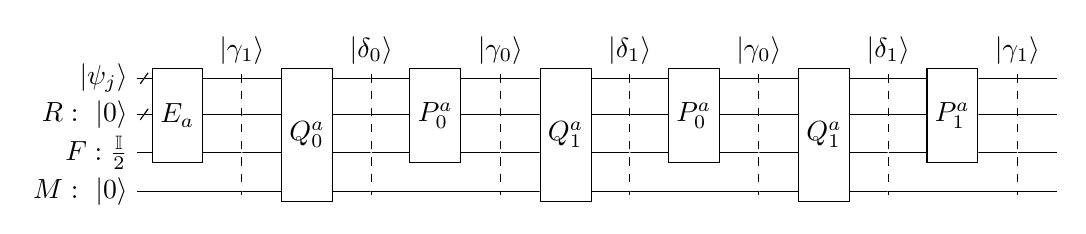
\begin{tikzpicture}
\begin{yquant*}
qubit {$\ket{\psi_j}$}  s;
qubit {$R:\ \ket{0}$} anc;
qubit {$F: \frac{\mathbb{I}}{2}$} f;
qubit {$M:\ \ket{0}$} m;
slash s;
slash anc;
hspace {0.1cm} -;
box {$E_a$} (s,anc,f);
["$\ket{\gamma_1}$"]
barrier (-);
box {$Q^a_0$} (s,anc,f, m);
["$\ket{\delta_0}$"]
barrier (-);
box {$P^a_0$} (s,anc,f);
["$\ket{\gamma_0}$"]
barrier (-);
box {$Q^a_1$} (s,anc,f, m);
["$\ket{\delta_1}$"]
barrier (-);
box {$P^a_0$} (s,anc,f);
["$\ket{\gamma_0}$"]
barrier (-);
box {$Q^a_1$} (s,anc,f, m);
["$\ket{\delta_1}$"]
barrier (-);
box {$P^a_1$} (s,anc,f);
["$\ket{\gamma_1}$"]
barrier (-);
\end{yquant*}
\end{tikzpicture}
\caption{A successfully completed rejection procedure. The same BSI-QPE registers $R, F$ are reused by $E_{ae}$ and every $P_s^{ae}$ and $Q_s^{ae}$; the qubit $M$ is reused by every $Q_s^{ae}$. This circuit corresponds to a term in $\mathcal{B}(2)[\rho]$ for $\{s_n\}=\{1,1\}$ and, within a single invariant subspace $\lambda$ (see Section~\ref{section:rejection}), occurs with probability $(1-p^{aej}_{\lambda})^4(p^{aej}_{\lambda})^2$. The state labels at the barriers denote the corresponding states of each invariant subspace.}
\label{fig:fullcircuit}
\end{figure*}

The iterative process proceeds as follows after measuring $s=0$ (reject) from the initial $Q_s^{ae}$ measurement: 
\begin{enumerate}
    \item Measure $P_s^{ae}$
        \begin{enumerate}
            \item If $s=1$ \textbf{terminate} as the state has returned to the approximate energy of the initial state.
            \item If $s=0$ continue.
        \end{enumerate}
    \item Measure $Q_s^{ae}$
    \item Repeat up to a maximum of $n^*$ iterations
\end{enumerate}


Before the algebra, here is the conclusion it establishes, so that the derivation can be read as a confirmation rather than a search. The two measurements $P^{ae}_s$ and $Q^{ae}_s$ do not scatter the state over the whole Hilbert space. They confine it to a family of mutually orthogonal \emph{two-dimensional} subspaces, and within any one of them the state simply ping-pongs between two pairs of vectors, $\ket{\gamma_0},\ket{\gamma_1}$ and $\ket{\delta_0},\ket{\delta_1}$, according to the four-state Markov chain of Fig.~\ref{fig:transitions}. Reaching $\ket{\gamma_1}$ means the rewind has succeeded and the state has returned to its original energy. Because the chain is this simple, the probability that $n^*$ attempts all fail can be read off directly, which is what Eq.~\eqref{eq:probabilty_of_rejection} does.

\begin{figure}
    \centering
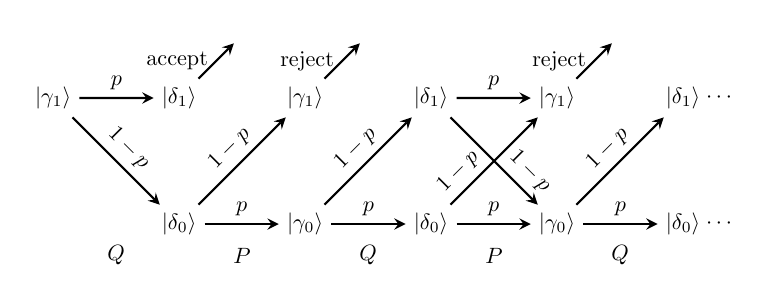
\begin{tikzpicture}[node distance=2cm, >=stealth, thick, scale=0.8, transform shape]
    \node (g-1t) at (0,2) {$|\gamma_1\rangle$};
    \node (s0t)  at (2,2) {$|\delta_1\rangle$};
    \node (s0)  at (2,0) {$|\delta_0\rangle$};
    \node (g0)  at (4,0) {$|\gamma_0\rangle$};
    \node (s1)  at (6,0) {$|\delta_0\rangle$};
    \node (g1)  at (8,0) {$|\gamma_0\rangle$};
    \node (s2)  at (10,0) {$|\delta_0\rangle$};
    \node (...1) at (10.6,0) {$\cdots$};
    \node (...2) at (10.6,2) {$\cdots$};
    
    \node (a) at (3,3) {};
    \node (r1) at (5,3) {};
    \node (r2) at (9,3) {};
    
    \node (g1t) at (4,2) {$|\gamma_1\rangle$};
    \node (s1t) at (6,2) {$|\delta_1\rangle$};
    \node (g2t) at (8,2) {$|\gamma_1\rangle$};
    \node (s2t) at (10,2) {$|\delta_1\rangle$};
    
    % Transitions
    \draw[->] (s0) -- node[above] {$p$} (g0);
    \draw[->] (g0) -- node[above] {$p$} (s1);
    \draw[->] (s1) -- node[above] {$p$} (g1);
    \draw[->] (g1) -- node[above] {$p$} (s2);
    
    \draw[->] (s0) -- node[above,sloped] {$1-p$} (g1t);
    \draw[->] (g0) -- node[above ,sloped] {$1-p$} (s1t);
    \draw[->] (s1) -- node[above left,sloped] {$1-p$} (g2t);
    \draw[->] (s1t) -- node[above] {$p$} (g2t);
    \draw[->] (g-1t) -- node[above] {$p$} (s0t);
    
    \draw[->] (s1t) -- node[above right,sloped] {$1-p$} (g1);
    \draw[->] (g1) -- node[above ,sloped] {$1-p$} (s2t);
    \draw[->] (g-1t) -- node[above ,sloped] {$1-p$} (s0);

    \draw[->] (s0t) -- node[left] {accept} (a);
    \draw[->] (g1t) -- node[left] {reject} (r1);
    \draw[->] (g2t) -- node[left] {reject} (r2);

    % Labels
    \node at (1,-0.5) {$Q$};
    \node at (3,-0.5) {$P$};
    \node at (5,-0.5) {$Q$};
    \node at (7,-0.5) {$P$};
    \node at (9,-0.5) {$Q$};
\end{tikzpicture}
    \caption{Markov chain showing the transition probability between the 4 states of a single invariant subspace $\lambda$ (with $p = p^{ae\lambda}$) upon each projective measurement. The full rejection process is a mixture of such chains weighted by $|c^{aej}_{\lambda}|^2$.}
    \label{fig:transitions}
\end{figure}

Let us consider the action of the rejection process on each eigenvector $\ket{\psi_j}$ of $H$. To handle the mixed initial state of $F$, purify $\frac{\mathbb{I}}{2}$ as $\ket{\Phi}_{FF'}=\frac{1}{\sqrt{2}}\sum_f\ket{f}_F\ket{f}_{F'}$, where the reference $F'$ is never acted upon. Conditioned on the outcome $(a,e)$, the corresponding pure post-measurement state is
\begin{equation}
    \frac{(E_{ae}\otimes\mathbb I_{F'})\ket{\psi_j}\ket{0}_R\ket{\Phi}_{FF'}\ket{0}_M}
    {\|(E_{ae}\otimes\mathbb I_{F'})\ket{\psi_j}\ket{0}_R\ket{\Phi}_{FF'}\ket{0}_M\|}
    = \sum_{\lambda} c_{\lambda}^{aej}\ket{\gamma_1^{ae \lambda}}.
\end{equation}
Tracing out $F'$ recovers the physical evolution from $\frac{\mathbb{I}}{2}$. Because $P_1^{ae}E_{ae}=E_{ae}$, this state is a $+1$ eigenstate of $P_1^{ae}$ (with all projectors implicitly extended by $\mathbb I_{F'}$). Furthermore, $P_1^{ae}$ commutes with $P^{ae}_1Q^{ae}_0P^{ae}_1$, so the two operators are jointly diagonalizable and the expansion above may be taken in their joint eigenstates. The untouched reference is absorbed into the degeneracy label $\lambda$.
Writing the eigenvalue of $\ket{\gamma^{ae\lambda}_1}$ as $1-p^{ae\lambda}$, we have: \begin{align}1-p^{ae\lambda}&=\bra{\gamma^{ae\lambda}_1}P^{ae}_1Q^{ae}_0P^{ae}_1\ket{\gamma^{ae\lambda}_1} \\&=\|Q^{ae}_0P^{ae}_1\ket{\gamma^{ae\lambda}_1}\|^2\\ &= 1-\|Q^{ae}_1\ket{\gamma^{ae\lambda}_1}\|^2
\end{align}
so $p^{ae\lambda} = \|Q^{ae}_1\ket{\gamma^{ae\lambda}_1}\|^2$, and the probability of accepting the update is given by the mixture $p_{aej} = \sum_{\lambda}|c^{aej}_{\lambda}|^2p^{ae\lambda}$. Therefore, for each $\lambda$ with $p^{ae\lambda} \in (0,1)$ we can define a two-dimensional invariant subspace as follows.
\begin{quote}
\emph{Notational warning.} For the remainder of this subsection the $ae\lambda$ labels are suppressed: we write $\ket{\gamma_1}$ for $\ket{\gamma^{ae\lambda}_1}$ and $p$ for $p^{ae\lambda}$. They are reinstated at Eq.~\eqref{eq:probabilty_of_rejection}.
\end{quote}
\begin{align}
    \ket{\delta_0} &= \frac{Q^{ae}_0P^{ae}_1\ket{\gamma_1}}{\sqrt{1-p}} &\ket{\delta_1} &= \frac{Q^{ae}_1P^{ae}_1\ket{\gamma_1}}{\sqrt{p}} \\
    \ket{\gamma_0} &= \frac{P^{ae}_0Q^{ae}_0\ket{\delta_0}}{\sqrt{p}} &\ket{\gamma_1} &= \frac{P^{ae}_1Q^{ae}_0\ket{\delta_0}}{\sqrt{1-p}}
\end{align}
From these definitions the following relations can be deduced:
\begin{align}
\begin{split}
\label{eq:deltagamma0}
    P^{ae}_1 \ket{\gamma_1} &= (Q^{ae}_0+Q^{ae}_1)P^{ae}_1 \ket{\gamma_1}\\
    &= Q^{ae}_0P^{ae}_1 \ket{\gamma_1}+Q^{ae}_1P^{ae}_1 \ket{\gamma_1}\\
    &= \sqrt{1-p} \ket{\delta_0} + \sqrt{p}\ket{\delta_1}\\
    Q^{ae}_0\ket{\delta_0} &= \sqrt{p} \ket{\gamma_0} + \sqrt{1-p} \ket{\gamma_1}
\end{split}
\end{align}
As $P^{ae}_1 \ket{\gamma_1} = \ket{\gamma_1}$ and $Q^{ae}_0\ket{\delta_0} = \ket{\delta_0}$ we can simplify the above and then through substitution deduce the remaining relations:
\begin{align}
\begin{split}
\label{eq:deltagamma1}
        \ket{\delta_1} &= -\sqrt{1-p} \ket{\gamma_0} + \sqrt{p} \ket{\gamma_1}\\
    \ket{\gamma_0} &= \sqrt{p} \ket{\delta_0} - \sqrt{1-p}\ket{\delta_1}
\end{split}
\end{align}
Therefore it is clear that each measurement transitions the state from one of $\ket{\delta_i}$ to one of $\ket{\gamma_i}$ or vice versa, whilst remaining within the same 2D invariant subspace. As the subspaces corresponding to different $\lambda$ are mutually orthogonal (which follows from the orthogonality of the $\ket{\gamma^{ae\lambda}_1}$ together with the relations above) and each is preserved by both measurements, the subspaces do not mix at any point during the rejection process. The probability of these transitions are trivially deduced from \eqref{eq:deltagamma0} and \eqref{eq:deltagamma1}, and can be seen in Fig.~\ref{fig:transitions}.

From this we can calculate the probability of attempting to reject and then failing the rejection process within a single invariant subspace to be $p(1-p)(p^2 +(1-p)^2)^{n^*}$. As the subspaces do not mix, the overall failure probability $p_a^{fail}$ is the corresponding mixture over subspaces (reinstating the suppressed labels):
\begin{equation}
   p_{aej}^{fail} =  \sum_{\lambda}|c^{aej}_{\lambda}|^2p^{ae\lambda}(1-p^{ae\lambda})((p^{ae\lambda})^2 +(1-p^{ae\lambda})^2)^{n^*}
\end{equation}
For all $p \in [0,1]$ we have: 
\begin{equation}
    p(1-p)(p^2 +(1-p)^2)^{n^*} \leq \frac{1}{2(n^*+1)} \left(\frac{n^*}{n^*+1}\right)^{n^*}
\end{equation}
Therefore, as $\sum_{\lambda}|c^{aej}_{\lambda}|^2=1$ we have:
\begin{equation}
    \label{eq:probabilty_of_rejection}
   p_{aej}^{fail} \leq \frac{1}{2(n^*+1)} \left(\frac{n^*}{n^*+1}\right)^{n^*} \leq \frac{1}{2n^*}
\end{equation}
If the rejection process fails then the whole algorithm fails irrecoverably and must be restarted from the original initial state.

Table~\ref{tab:resources} collects the cost of one round. The row worth noting is the third from last: the excess over an exact energy readout is only $c = O(\log(\frac{1}{\nu}\log n^*))$ qubits, which is the sense in which the resource threshold for Quantum Metropolis sampling is lower than previously believed. The last row is the price paid for reversibility: the rewinding loop can invoke phase estimation up to $O(n^*)$ times in the worst case. The typical cost is far smaller, since $\|\mathcal{B}(n)[\sigma_G]\|_* = O(n^{-2})$ makes the expected number of rewinding iterations only $O(\log n^*)$; the cap $n^*$ bounds the tail of that distribution, and Eq.~\eqref{eq:probabilty_of_rejection} bounds the probability of hitting it.

\begin{table}[b]
\caption{Resources for one round of the algorithm. $m$ denotes the number of system qubits (as in Section~\ref{section:boostedphaseestimation}), $\eta$ the size of the energy register, and $n^*$ the rewinding cap. One BSI-QPE invocation costs $O(2^{\eta})$ applications of $U=e^{iHt/2}$, i.e.\ a total evolution time $O(2^{\eta}/\|H\|)$ at $t=\frac{1}{16\|H\|}$.}
\label{tab:resources}
\begin{ruledtabular}
\begin{tabular}{ll}
Resource & Count \\
\hline
System qubits & $m$ \\
Energy register $R$ & $\eta$ \\
Direction qubit $F$, rotation qubit $M$ & $2$ \\
Extra ancillas beyond an exact readout & $c = O(\log(\frac{1}{\nu}\log n^*))$ \\
Applications of $U$ per BSI-QPE & $O(2^{\eta})$ \\
BSI-QPE invocations per round & $\leq 4n^*+6$ \\
\end{tabular}
\end{ruledtabular}
\end{table}



\label{section:rejection}

\section{Why it works}
\label{section:why}
The classical Metropolis--Hastings algorithm works by constructing a Markov chain through proposing and accepting/rejecting moves with probabilities determined by the energy difference between the initial and modified states. The transition matrix of this Markov chain is in detailed balance with respect to the Gibbs state, implying that the Gibbs state is a fixed point of the Markov chain. As the Markov chain is also ergodic, it is known that it must have a single unique fixed point and converge towards it. Therefore, the Markov chain converges to the Gibbs state.

In the quantum Metropolis algorithm we similarly construct a quantum Markov chain by proposing and accepting or rejecting moves based on energy differences. Because the energy differences cannot be resolved exactly, we cannot prove exact detailed balance and instead use a notion of approximate quantum detailed balance (Theorem~\ref{theorem:quantumapproximatedeatildedbalance}) that incorporates additive errors from the nonzero, exponentially suppressed tails of BSI-QPE. We use this theorem to establish that the Gibbs state is approximately invariant. Further choosing the update set $\{C\}$ to be universal ensures ergodicity and hence the uniqueness of the fixed point \cite{Temme_2011}. The closeness of the actual fixed point to this approximately invariant point additionally depends on the mixing properties of the channel. We formalise these statements into the main result of the paper. Informally, it says: \emph{one round of the algorithm moves the Gibbs state only a little, and the two ways it can move are both controllable --- by adding ancilla qubits, and by allowing more rewinding attempts.} Formally:

\begin{theorem}
\label{theorem:main}
Let $\mathcal{E}$ be one update round of the quantum Metropolis algorithm of Section~\ref{section:algorithm}, implemented with $\eta$ ancillas, evolution time $t = \frac{1}{16\|H\|}$, rewinding cap $n^*$, an update measure satisfying $d\mu(C)=d\mu(C^{\dagger})$, and window functions satisfying the conditions of Appendix~\ref{section:appendix} with truncation bandwidth $\mu = O(\frac{1}{\nu}\log n^*)$, $\mu < \frac{2^{\eta}}{96\pi}$. Then
\begin{equation}
   \|\mathcal{E}[\sigma_G] - \sigma_G\|_* = O\left(\max\left( n^{*\frac{7}{2}}\sqrt{\frac{\beta\|H\| }{2^{\eta}}}\mu^{\frac{3}{2}},\frac{1}{n^*}\right)\right).
\label{eq:theoremmain}
\end{equation}
If, in addition, $\mathcal{E}$ is strictly trace-norm contracting with factor $k<1$, then $\mathcal{E}$ has a unique fixed point $\sigma^*$, is approached exponentially fast, and $\|\sigma^*-\sigma_G\|_* \leq \frac{1}{1-k}\|\mathcal{E}[\sigma_G] - \sigma_G\|_*$ (Theorem~\ref{theorem:error_bound}).
\end{theorem}

The two terms in Eq.~\eqref{eq:theoremmain} have quite different origins, and it is worth separating them before the proof. The first, $n^{*\frac{7}{2}}\sqrt{\beta\|H\|2^{-\eta}}\mu^{\frac{3}{2}}$, is the residual \emph{bias} left by an imperfect energy estimate: the acceptance probability is computed from a readout that is only accurate to within the bandwidth $\mu$, so detailed balance holds only up to a multiplicative error, and every extra rewinding attempt gives that error another chance to act. It shrinks exponentially in the number of ancilla qubits $\eta$. The second, $1/n^*$, is the probability that the rewind never terminates and the whole run must be discarded (Eq.~\eqref{eq:probabilty_of_rejection}); it shrinks as the cap $n^*$ is raised. The two therefore pull in opposite directions in $n^*$, and balancing them at $n^{*\frac{9}{2}} \sim \sqrt{2^{\eta}/(\beta\|H\|)}\,\mu^{-\frac32}$ gives the best per-round error for a given ancilla budget. Since $\mu$ enters only polynomially while $\epsilon_{\Delta}$ falls as $e^{-\nu\mu}$, the bandwidth may be taken as small as $\mu = O(\frac{1}{\nu}\log n^*)$, which is what produces the logarithmic qubit count of Eq.~\eqref{eq:headline}.

The proof of this theorem occupies the remainder of this section and is broken down into a number of steps. First, in Section~\ref{section:detailedbalancedef} we define our approximate detailed balance criteria which allow us to consider each branch of the original $\mathcal{E}$ CP-map separately. We then proceed in Section~\ref{section:accept} and \ref{section:rejectionbranch} to prove the acceptance and rejection branches of our update step satisfy our branch-wise approximate detailed balance criteria. In both instances we follow the same four steps, sketched in Fig.~\ref{fig:proofsteps}:
\begin{enumerate}
    \item \textbf{Truncate.} We replace $\hat \alpha$, $\hat \beta$ by their band-limited versions $\tilde \alpha$, $\tilde \beta$ as in Lemma~\ref{lemma:0}. Then, we use Lemma~\ref{lemma:3} to bound the diamond-norm difference between the original $E^{ae}$, $P_s^{ae}$, $Q_s^{ae}$ measurements and their band-limited replacements. Using Lemma~\ref{lemma:composition} we combine these bounds on the error of each measurement into a diamond-norm bound on the difference between the full band-limited map and the original.
    \item \textbf{Support.} Band-limiting means that only a narrow set of index combinations contributes. We now find that set, because the relabelling of the next step is only well defined on it. By considering the restricted support of the band-limited operations we are able to find the subset of possible measurement outcomes when acting upon a given input state.
    \item \textbf{Reverse Histories.} By relabelling the indices corresponding to the measurement outcomes we are able to (approximately) relate a branch of the adjoint map with one of the original map up to the Boltzmann factors. This is the step that makes the argument work, and it is where a reader should slow down: a branch of the adjoint map describes the round run backwards, and the relabelling is nothing more than reading the measurement record from the end to the beginning. In the acceptance branch this requires that the move distribution weights $C$ and $C^{\dagger}$ equally ($d\mu(C) = d\mu(C^{\dagger})$). For the rejection branch it additionally requires demonstrating that perturbing all of the rotations by $z$ (which has small modular norm due to the restricted support) yields a controllable error on the full map.
    \item \textbf{Reweight.} Using the restricted support of the band-limited BSI-QPE we finish relating the adjoint map with the original map by exchanging the Boltzmann factors up to a multiplicative error. This is what turns the exact detailed balance of the classical algorithm into the approximate statement of Lemma~\ref{lemma:1}.
\end{enumerate}

\begin{figure}[t]
\centering
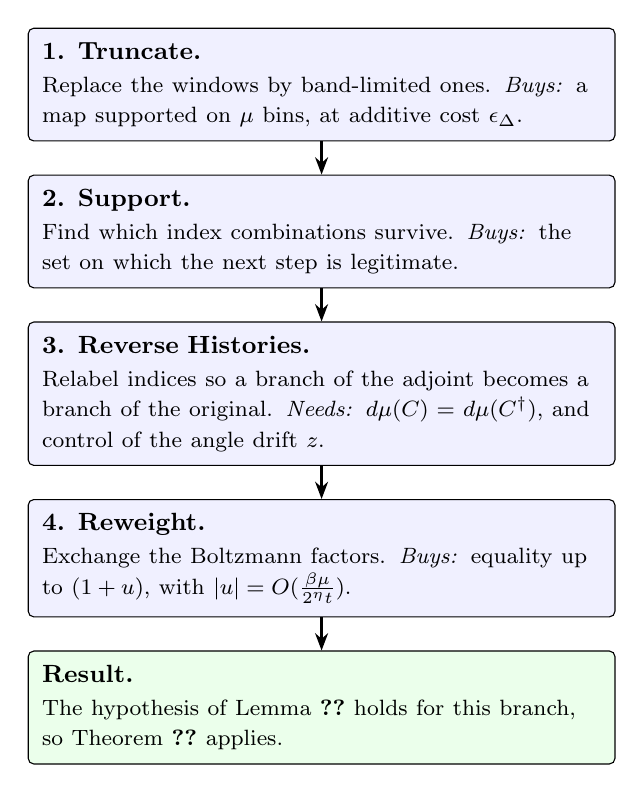
\begin{tikzpicture}[
  font=\small, node distance=0.42cm,
  st/.style={draw, rounded corners=2pt, align=left, text width=7.1cm, inner sep=5pt},
  ar/.style={-{Stealth[length=2.2mm]}, thick}
]
\node[st, fill=blue!6]   (s1) {\textbf{1. Truncate.}\\[1pt]\footnotesize Replace the windows by band-limited ones. \emph{Buys:} a map supported on $\mu$ bins, at additive cost $\epsilon_{\Delta}$.};
\node[st, fill=blue!6, below=of s1] (s2) {\textbf{2. Support.}\\[1pt]\footnotesize Find which index combinations survive. \emph{Buys:} the set on which the next step is legitimate.};
\node[st, fill=blue!6, below=of s2] (s3) {\textbf{3. Reverse Histories.}\\[1pt]\footnotesize Relabel indices so a branch of the adjoint becomes a branch of the original. \emph{Needs:} $d\mu(C)=d\mu(C^{\dagger})$, and control of the angle drift $z$.};
\node[st, fill=blue!6, below=of s3] (s4) {\textbf{4. Reweight.}\\[1pt]\footnotesize Exchange the Boltzmann factors. \emph{Buys:} equality up to $(1+u)$, with $|u|=O(\frac{\beta\mu}{2^{\eta}t})$.};
\node[st, fill=green!8, below=of s4] (s5) {\textbf{Result.}\\[1pt]\footnotesize The hypothesis of Lemma~\ref{lemma:1} holds for this branch, so Theorem~\ref{theorem:quantumapproximatedeatildedbalance} applies.};
\draw[ar] (s1) -- (s2); \draw[ar] (s2) -- (s3); \draw[ar] (s3) -- (s4); \draw[ar] (s4) -- (s5);
\end{tikzpicture}
\caption{The four steps of the convergence proof, applied once to the acceptance branch (Section~\ref{section:accept}) and once to the rejection branch (Section~\ref{section:rejectionbranch}). Each step is stated with what it buys, since the steps are only useful in sequence: truncation makes the support finite, the support makes the relabelling well defined, the relabelling turns the adjoint into the original map, and the reweighting removes the last discrepancy between them.}
\label{fig:proofsteps}
\end{figure}

We combine the output of Lemma~\ref{lemma:1} for the band-limited acceptance and rejection branches with the Lemma~\ref{lemma:composition} bounds on the truncation. We then feed these results into Theorem~\ref{theorem:quantumapproximatedeatildedbalance} to combine with the failure to reject branch.
\subsection{Approximate Quantum Detailed Balance}
\label{section:detailedbalancedef}
Here we present a modified formulation of approximate quantum detailed balance which allows for additive errors to be introduced from the truncation step of the proof. 

For any completely positive map $\mathcal{M}$ ($\mathcal{M}[\rho] =\sum_{j}  A_{j}\rho  A^{\dagger}_{j}$) and density matrix $\sigma$, we define $\mathcal{M}_{\sigma}[\rho] =\sum_{j}  A_{j}\sigma^{\frac{1}{2}}\rho\sigma^{\frac{1}{2}}  A^{\dagger}_{j}$, $\mathcal{M}^{\dagger}[\rho] = \sum_j A^{\dagger}_j \rho A_j$ and $ \mathcal{M}^*_{\sigma}[\rho] = \sum_{j} \sigma^{\frac{1}{2}}A^{\dagger}_{j}\rho A_{j}\sigma^{\frac{1}{2}} = \sigma^{\frac{1}{2}}\mathcal{M}^{\dagger}[\rho]\sigma^{\frac{1}{2}}$.
\begin{lemma}[Branch-wise Approximate Quantum Detailed Balance Criteria]
\label{lemma:1}
Let $\mathcal{M}$ and $\mathcal{M'}$ be a completely positive maps on $d$-dimensional density matrices admitting the same decomposition $\mathcal{M} = \sum_{c\in\mathcal{X}} \mathcal{M}_c$, $\mathcal{M'} = \sum_{c\in\mathcal{X}} \mathcal{M'}_c$ into completely positive maps $\mathcal{M}_c$ and $\mathcal{M}'_c$, and let $\sigma = \sum_j \sigma_j \ket{\psi_j}\bra{\psi_j}$ be a density matrix diagonal in the orthonormal basis $\{\ket{\psi_j}\}$. Suppose there exists a bijection $c \mapsto c'$ of $\mathcal{X}$ such that, for every $j,c,l,m$,
\begin{multline}
    \bra{\psi_m}\mathcal{M}'^*_{c'\sigma}[\ket{\psi_j}\bra{\psi_j}]\ket{\psi_l}
    =\\(1+u^{jc}_m)(1+ u^{jc}_l)
    \bra{\psi_m}\mathcal{M}_{c\sigma}[\ket{\psi_j}\bra{\psi_j}]\ket{\psi_l}
    \label{eq:approximate_quantum_detailed_balance_condition}
\end{multline}
where the $u^{jc}_l$ are real and satisfy $|u^{jc}_l| \leq \epsilon_m$. Then:
 \begin{equation}
    \|\mathcal{M}'^*_{\sigma}[\mathbb{I}]-\mathcal{M}[\sigma] \|_* \leq (2\epsilon_m+\epsilon_m^2)\|\mathcal{M}[\sigma]\|_* \label{eq:lemma2output}
\end{equation}
where $\|\cdot\|_*$ is trace-norm.
\end{lemma}

\begin{proof}
    By definition $\mathcal{M}[\sigma]=\mathcal{M}_{\sigma}[\mathbb{I}]$. By linearity and the bijectivity of $c \mapsto c'$:
    \begin{equation}
        \mathcal{M}'^*_{\sigma}[\mathbb{I}] = \sum_{j,c}\mathcal{M}'^*_{c\sigma}[\ket{\psi_j}\bra{\psi_j}] = \sum_{j,c}\mathcal{M}'^*_{c'\sigma}[\ket{\psi_j}\bra{\psi_j}]
    \end{equation}
    Define $N^{jc} = \mathcal{M}_{c\sigma}[\ket{\psi_j}\bra{\psi_j}]$ and $D^{jc}=\sum_l(1+u_l^{jc})\ket{\psi_l}\bra{\psi_l}$. Equation~\eqref{eq:approximate_quantum_detailed_balance_condition} is then the operator identity $\mathcal{M}'^*_{c'\sigma}[\ket{\psi_j}\bra{\psi_j}]=D^{jc}N^{jc}D^{jc}$. Moreover, $N^{jc}$ is positive semidefinite as $\mathcal{M}_c$ is completely positive, so that $\mathcal{M}_{\sigma}[\mathbb{I}] = \sum_{j,c}N^{jc}$. Writing $V^{jc} = D^{jc}-\mathbb{I}$, which satisfies $\|V^{jc}\|\leq\epsilon_m$, we have:
    \begin{equation}
        D^{jc}N^{jc}D^{jc} - N^{jc} = V^{jc}N^{jc} + N^{jc}V^{jc} + V^{jc}N^{jc}V^{jc}
    \end{equation}
    By H\"older's inequality each term is bounded in trace-norm as:
    \begin{equation}
        \|V^{jc}N^{jc}\|_* \leq \|V^{jc}\|\|N^{jc}\|_* \leq \epsilon_m Tr[N^{jc}]
    \end{equation}
    and similarly for the remaining terms. Therefore, by the triangle inequality:
    \begin{align}
        \|\mathcal{M}'^*_{\sigma}[\mathbb{I}]-\mathcal{M}_\sigma[\mathbb{I}]\|_* &\leq \sum_{j,c}\left(\|D^{jc}N^{jc}D^{jc}-N^{jc}\|_*\right)\\
        &\leq (2\epsilon_m+\epsilon_m^2)\sum_{j,c}Tr[N^{jc}] 
    \end{align}
    Finally, as each $N^{jc}$ is positive semidefinite:
    \begin{equation}
        \sum_{j,c}Tr[N^{jc}] = Tr[\mathcal{M}_{\sigma}[\mathbb{I}]] = Tr[\mathcal{M}[\sigma]] = \|\mathcal{M}[\sigma]\|_*
    \end{equation}
\end{proof}
\begin{remark}[Relation to $\sigma$-detailed balance]
Lemma~\ref{lemma:1} is an approximate, branch-resolved form of the quantum detailed balance conditions used in the Gibbs-sampler literature. The map $\mathcal{M}^*_{\sigma}$ is the adjoint of $\mathcal{M}$ with respect to the $\sigma^{1/2}$-weighted (KMS-type) inner product $\braket{X,Y}_{\sigma} = Tr[X^{\dagger}\sigma^{\frac{1}{2}}Y\sigma^{\frac{1}{2}}]$, and exact quantum detailed balance of a channel is self-adjointness in this inner product \cite{temme2010chi,chen2023quantumthermalstatepreparation}. Setting $u^{jc}_l \equiv 0$ and $\mathcal{M}' = \mathcal{M}$ in Eq.~\eqref{eq:approximate_quantum_detailed_balance_condition} recovers exactly that notion, branch-paired by $c \mapsto c'$; the lemma weakens it multiplicatively, per branch, which is what an imperfect energy estimate can actually deliver.
\end{remark}

We will use the above Lemma to show that our band-limited maps satisfy \eqref{eq:lemma2output}. We will then combine this with the additive error ($\epsilon_a$) between the original map and the band-limited map to produce an equation of the following form for both the acceptance and rejection branches:
\begin{equation}
    \|\mathcal{M}'^*_{\sigma}[\mathbb{I}]-\mathcal{M}[\sigma] \|_* \leq (2\epsilon_m+\epsilon_m^2)\|\mathcal{M}[\sigma]\|_* + \epsilon_a
\end{equation}
We will then combine these into one overall approximate quantum detailed balance condition using the following theorem.
\begin{theorem}[Approximate Quantum Detailed Balance]
\label{theorem:quantumapproximatedeatildedbalance}
Given a completely positive trace preserving map $\mathcal{E}$ on $d$-dimensional density matrices constructed from a sum of completely positive maps $\mathcal{M}_j$:
\begin{equation}
    \mathcal{E}[\rho] = \sum_j \mathcal{M}_j[\rho]
\end{equation}
If for every $\mathcal{M}_j$ and the same given density matrix $\sigma$ we have:
\begin{equation}
    \|\mathcal{M}^*_{j\sigma}[\mathbb{I}]-\mathcal{M}_{j}[\sigma]\|_* \leq \epsilon^j
\end{equation}
 then we have:
\begin{equation}
     \|\mathcal{E}[\sigma]-\sigma\|_* \leq \sum_j\min\left(\epsilon^j, 2\|\mathcal{M}_j[\sigma]\|_*\right)
\end{equation}
\end{theorem}
\begin{proof}
    By the triangle inequality we have:
    \begin{equation}
        \|\mathcal{E}^*_{\sigma}[\mathbb{I}]-\mathcal{E}[\sigma]\|_* \leq \sum_j \|\mathcal{M}^*_{j\sigma}[\mathbb{I}]-\mathcal{M}_{j}[\sigma]\|_*
    \end{equation}
    As $\mathcal{E}$ is trace-preserving, we know that:
    \begin{equation}
        \mathcal{E}^*_{\sigma}[\mathbb{I}] = \sum_{j} \sigma^{\frac{1}{2}}A^{\dagger}_{j} A_{j}\sigma^{\frac{1}{2}} = \sigma
    \end{equation}
    Therefore,
    \begin{equation}
        \|\sigma - \mathcal{E}[\sigma]\|_* \leq \sum_j \|\mathcal{M}^*_{j\sigma}[\mathbb{I}]-\mathcal{M}_{j}[\sigma]\|_*
    \end{equation}
    By assumption we have that for all $j$:
    \begin{equation}
        \|\mathcal{M}^*_{j\sigma}[\mathbb{I}]-\mathcal{M}_{j}[\sigma]\|_* \leq \epsilon^j
    \end{equation}
    Further, as both
$\mathcal{M}_{j,\sigma}^{*}[\mathbb{I}]$ and
$\mathcal{M}_j[\sigma]$ are positive semidefinite:
    \begin{align}
        \|\mathcal{M}^*_{j\sigma}[\mathbb{I}]\|_* &= Tr\left[\sum_l \sigma^{\frac{1}{2}} K_{jl}^{\dagger} \mathbb{I} K_{jl} \sigma^{\frac{1}{2}}\right]\\
        &= Tr\left[\sum_l K_{jl}\sigma K_{jl}^{\dagger}\right]\\
        &= \|\mathcal{M}_{j}[\sigma]\|_*
    \end{align}
    Therefore,
    \begin{equation}
         \|\mathcal{M}^*_{j\sigma}[\mathbb{I}]-\mathcal{M}_{j}[\sigma]\|_* \leq 2\|\mathcal{M}_{j}[\sigma]\|_*
    \end{equation}
    Hence,
    \begin{equation}
        \|\sigma-\mathcal{E}[\sigma]\|_* \leq \sum_j \min \left(\epsilon^j, 2\|\mathcal{M}_{j}[\sigma]\|_*\right)
    \end{equation}
\end{proof}

\begin{widetext}
\subsection{Proof of Theorem~\ref{theorem:main}}
We must first express $\mathcal{E}$ as a completely positive trace preserving map:
\begin{equation}
    \mathcal{E}[\rho] = \mathcal{A}[\rho] + \sum_{n=0}^{n^*} \mathcal{B}(n)[\rho] + \mathcal{C}[\rho]
\end{equation}
where $\mathcal{A}$ corresponds to acceptance, $\mathcal{B}(n)$ to successful rejection after $n$ iterations and $\mathcal{C}$ to failing to reject after $n^*$ iterations. Let $\Omega_{RFM} =\ket{0}\bra{0}_R\otimes \frac{\mathbb{I}_F}{2}\otimes\ket{0}\bra{0}_M$ denote the initial state of the persistent ancillas. All occurrences of $E_{ae}$, $P_s^{ae}$, $Q_s^{ae}$ and $L_b^{ade}$ below act on this common ancillary space, with identities on any register on which a given operator acts trivially. Then
\begin{equation}
    \mathcal{A}[\rho] = \int  Tr_{RFM}\bigg[\sum_{a,b,d,e}L_b^{ade} E_{ae} ( \rho\otimes \Omega_{RFM}) 
     E_{ae}L^{ade\dagger}_b\bigg]d\mu(C)
\end{equation}
\begin{equation}
    \mathcal{B}(n)[\rho] = \int Tr_{RFM}\bigg[\sum_{a,e,\{s\}}P^{ae}_1Q^{ae}_{s_n}\ldots P^{ae}_0Q^{ae}_{s_1}P^{ae}_0Q^{ae}_0E_{ae} ( \rho\otimes \Omega_{RFM})E_{ae}Q^{ae}_0P^{ae}_0Q^{ae}_{s_1}P^{ae}_0\ldots Q^{ae}_{s_n}P^{ae}_1\bigg]d\mu(C)
\end{equation}
\begin{equation}
    \mathcal{C}[\rho] = \rho_0 \int Tr\bigg[\sum_{a,e,\{s\}}P^{ae}_0Q^{ae}_{s_{n^*}}\ldots P^{ae}_0Q^{ae}_{s_1}P^{ae}_0Q^{ae}_0E_{ae} ( \rho\otimes \Omega_{RFM})E_{ae}Q^{ae}_0P^{ae}_0Q^{ae}_{s_1}P^{ae}_0\ldots Q^{ae}_{s_{n^*}}P^{ae}_0\bigg]d\mu(C) 
\end{equation}
where $\rho_0$ is the initial state the overall Metropolis algorithm was started from. 

 % To do so we will consider approximations to $\mathcal{A}$ and $\mathcal{B}(n)$ in which we have substituted $\tilde \alpha, \tilde \beta$ for $\hat \alpha, \hat \beta$. Under this substitution $G^{pq}_j$ becomes $\tilde G^{pq}_j$ such that $\|\tilde G^{pq}_j\| =0$ for all $|p-q\pm\frac{2^{\eta}}{2\pi}E_jt|_{2^{\eta}} > \mu$. Then using Lemma~\ref{lemma:3} we will show that $\|\tilde{\mathcal{A}}-\mathcal{A}\|_{\diamond} \leq \epsilon$ and $\|\tilde{\mathcal{B}}(n)-\mathcal{B}(n)\|_{\diamond} \leq \epsilon$, and hence transfer the bounds from the approximated maps to the true maps. We will not evaluate Lemma~\ref{lemma:1} for $\mathcal{C}$, but rather bound its contribution in Theorem~\ref{theorem:quantumapproximatedeatildedbalance} by its trace-norm. 
\subsubsection{Acceptance Branch}
\label{section:accept}
\textbf{Truncate.} We begin with $\mathcal{A}$ and perform a truncation to $\tilde{\mathcal{A}}$ by substituting $\tilde \alpha, \tilde \beta$ for $\hat \alpha, \hat \beta$. Under this substitution $G^{pq}_j$ becomes $\tilde G^{pq}_j$ such that $\|\tilde G^{pq}_j\| =0$ for all $|p-q\pm\frac{2^{\eta}}{2\pi}E_jt|_{2^{\eta}} > \mu$.  By Lemma~\ref{lemma:0} this produces a modified operator $\widetilde{\text{BSI-QPE}}$ such that $\|\widetilde{\text{BSI-QPE}}- \text{BSI-QPE}\| \leq \frac{2\epsilon_{\Delta}}{\sqrt{2^{\eta}}}$. In Appendix~\ref{section:appendixTrunc} we prove the following Lemma that relates an operator norm bound approximation of a Kraus operator to a diamond-norm bound in the approximation of the CP-map.
\begin{lemma}
\label{lemma:3}
Let $\{D_s\}_{s\in S}$ be mutually orthogonal projectors satisfying $\sum_{s\in S} D_s \leq \mathbb{I}$. Given unitaries $U$ and $V$, define the measurement $K_s = U^{\dagger}D_s V$ and CP map $\mathcal{K}[\rho] = \sum_{s \in S} K_s\rho K_s^{\dagger}$. Further, given operators $\tilde U, \tilde V$, define approximate measurement operators $\tilde K_s = \tilde U^{\dagger}D_s \tilde V$ and the approximate map $\tilde{\mathcal{K}}[\rho] = \sum_{s \in S} \tilde K_s\rho \tilde K_s^{\dagger}$. If $\|U-\tilde U\| \leq \epsilon<\frac14$ and $\|V-\tilde V\| \leq \epsilon<\frac14$, then 
\begin{equation}
    \|\mathcal{K} - \tilde{\mathcal{K}}\|_{\diamond} \leq 6\epsilon
\end{equation}
\end{lemma}
We can see that $\mathfrak{E}[\rho] =  E \rho E$, $\mathcal{P}_S[\rho] = \sum_{s\in S} P_s \rho P_s$, $\mathcal{Q}_S[\rho] = \sum_{s\in S} Q_s \rho Q_s$ and $\mathcal{L}[\rho] = \sum_{bd} L_{bd} \rho L^{\dagger}_{bd}$ are all CP maps of the form described in Lemma~\ref{lemma:3}. Here we have dropped the $ae$ superscript from $E$, $P_s$, $Q_s$ and $L_{bd}$ by postponing the corresponding classical conditioning until the end of the circuit: the outcomes are stored in additional pointer registers, and the later operations are controlled on those registers. This is only a proof technique and does not alter the persistent registers $R, F$ used by $E$, $P$, $L$ and $Q$. As $E$ and $P_s$ can be written as $\text{BSI-QPE}^{\dagger}\cdot D_s\cdot\text{BSI-QPE}$, $Q = C^{\dagger}\cdot\text{BSI-QPE}^{\dagger}\cdot D_s\cdot \text{BSI-QPE}\cdot C$ and $L = \text{BSI-QPE}^{\dagger}\cdot W\cdot D_s\cdot \text{BSI-QPE}\cdot C$ we can use the operator norm bound $\|\widetilde{\text{BSI-QPE}}- \text{BSI-QPE}\| \leq \frac{2\epsilon_{\Delta}}{\sqrt{2^{\eta}}}$ to see that:
\begin{equation}
    \|\mathfrak{E} - \tilde{\mathfrak{E}}\|_{\diamond} \leq \frac{12\epsilon_{\Delta}}{\sqrt{2^{\eta}}} \qquad\|\mathcal{P}_S - \tilde{\mathcal{P}}_S\|_{\diamond} \leq \frac{12\epsilon_{\Delta}}{\sqrt{2^{\eta}}} \qquad\|\mathcal{Q}_S - \tilde{\mathcal{Q}}_S\|_{\diamond} \leq \frac{12\epsilon_{\Delta}}{\sqrt{2^{\eta}}}  \qquad\|\mathcal{L} - \tilde{\mathcal{L}}\|_{\diamond} \leq \frac{12\epsilon_{\Delta}}{\sqrt{2^{\eta}}} 
    \label{eq:bound_on_component_maps}
\end{equation}
We can combine these bounds using the following Lemma which we also prove in Appendix~\ref{section:appendixTrunc}.
\begin{lemma}
\label{lemma:composition}
Let $\mathcal{M}_1, \ldots, \mathcal{M}_k$ be completely positive trace-non-increasing maps and let $\tilde{\mathcal{M}}_1, \ldots, \tilde{\mathcal{M}}_k$ be completely positive maps with $\|\mathcal{M}_i - \tilde{\mathcal{M}}_i\|_{\diamond} \leq \varepsilon$ for all $i$. Then
\begin{equation}
    \|\mathcal{M}_k \circ \cdots \circ \mathcal{M}_1 - \tilde{\mathcal{M}}_k \circ \cdots \circ \tilde{\mathcal{M}}_1\|_{\diamond} \leq (1+\varepsilon)^k - 1 \leq e k \varepsilon,
\end{equation}
the last inequality holding whenever $k\varepsilon \leq 1$.
\end{lemma}
We can write $\mathcal{A}[\rho] = \mathcal{L} \circ \mathcal{E}[\rho]$, and hence by Lemma~\ref{lemma:composition} and \eqref{eq:bound_on_component_maps} we have:
\begin{equation}
    \|\mathcal{A} - \tilde{\mathcal{A}}\|_{\diamond} \leq 24e \frac{\epsilon_{\Delta}}{\sqrt{2^{\eta}}}
\end{equation}
As $\mathcal{M}^*_{\sigma}[\mathbb{I}] = \sigma^{\frac{1}{2}}\mathcal{M}^{\dagger}[\mathbb{I}]\sigma^{\frac{1}{2}}$, where $\mathcal{M}^{\dagger}$ denotes the adjoint map, and $\|\mathcal{M}^{\dagger}[X] - \tilde{\mathcal{M}}^{\dagger}[X]\| \leq \|\mathcal{M}-\tilde{\mathcal{M}}\|_{\diamond}\|X\|$ (by the duality of the $1\to1$ and $\infty\to\infty$ superoperator norms), H\"older's inequality gives:
\begin{equation}
    \|\mathcal{A}^*_{\sigma_G}[\mathbb{I}] - \tilde{\mathcal{A}}^*_{\sigma_G}[\mathbb{I}]\|_* \leq Tr[\sigma_G]\,\|\mathcal{A}^{\dagger}[\mathbb{I}] - \tilde{\mathcal{A}}^{\dagger}[\mathbb{I}]\| \leq 24e\frac{\epsilon_{\Delta}}{\sqrt{2^{\eta}}}
    \label{eq:AAtildeclose1}
\end{equation}
and directly:
\begin{equation}
    \|\mathcal{A}[\sigma_G] - \tilde{\mathcal{A}}[\sigma_G]\|_* \leq \|\mathcal{A}-\tilde{\mathcal{A}}\|_{\diamond} \leq 24e\frac{\epsilon_{\Delta}}{\sqrt{2^{\eta}}}
    \label{eq:AAtildeclose2}
\end{equation}
\textbf{Support.} Band-limiting has bought us something specific: only a narrow set of index combinations can now contribute, and the relabelling of the next step only makes sense on that set. We therefore identify it.

Writing $\sigma_G = \frac{1}{Z}\sum_j e^{-\beta E_j} \ket{\psi_j}\bra{\psi_j}$ with $\ket{\psi_j}$ the eigenstates of $H$, and expanding $\tilde{\mathcal{A}}_{\sigma_G}$ and its adjoint in this eigenbasis, gives Eqs.~\eqref{eq:Arho} and~\eqref{eq:A*rho} of Appendix~\ref{section:appendixDetail}. Due to the restricted support of $\tilde \alpha$ and $\tilde \beta$ we have that $\|\tilde G^{bp\dagger}_{j}\ket{d}\bra{d}\tilde G^{bq}_{j}\| = 0$ for $|p-q|_{2^{\eta}} > 2\mu$. Further, we have $\|\tilde G^{ap \dagger}_j \ket{e}\| = 0$ if $|a-p-(-1)^e\frac{2^{\eta}}{2\pi}E_{j}t|_{2^{\eta}} > \mu$. Hence, we can restrict the summations in Eq.~\eqref{eq:Arho}  to the set $a,b,d,e,p_1,q_1,p_2 \in \chi_{jklm}$ of summation indices satisfying
\begin{equation}
\begin{aligned}
    |a-(-1)^e\frac{2^{\eta}}{2\pi}E_jt|_{2^{\eta}} &\leq \mu  &|a-(-1)^e\frac{2^{\eta}}{2\pi}E_kt|_{2^{\eta}} &\leq \mu\\
       |b-p_2-(-1)^{d}\frac{2^{\eta}}{2\pi}E_mt|_{2^{\eta}}& \leq \mu&|b-p_2-(-1)^{d}\frac{2^{\eta}}{2\pi}E_lt|_{2^{\eta}} &\leq \mu \\
    |p_1|_{2^{\eta}}&\leq 2\mu&  |q_1|_{2^{\eta}}&\leq 2\mu \\
    |p_2-p_1|_{2^{\eta}}&\leq 2\mu&  |p_2-q_1|_{2^{\eta}}&\leq 2\mu \\
\end{aligned}
\end{equation}
Applying the modular triangle inequality separately along the two paths gives the following necessary conditions, which define a superset $\chi_{jklm}'\supset\chi_{jklm}$:
\begin{equation}
\label{eq:condJ}
\begin{aligned}
    \left|(-1)^db -(-1)^ea-\frac{2^{\eta}t}{2\pi}(E_m-E_j)\right|_{2^{\eta}}&\leq 6\mu,\\
    \left|(-1)^db -(-1)^ea-\frac{2^{\eta}t}{2\pi}(E_l-E_k)\right|_{2^{\eta}}&\leq 6\mu,
\end{aligned}
\end{equation}
As $|E_j| \leq \|H\|$, if we choose $t = \frac{1}{16\|H\|}$ and $\mu < \frac{2^{\eta}}{96\pi}$ so that $E_j$ satisfies $-\frac{1}{8t} + 3\frac{2\pi}{2^{\eta}t}\mu < E_j < \frac{1}{8t} - 3\frac{2\pi}{2^{\eta}t}\mu$, then we have that $-2^{\eta-2}+6\mu < \frac{2^{\eta}t}{2\pi}(E_i -E_j) < 2^{\eta-2}-6\mu$ for all $i$ and $j$. Hence, we can restrict the ranges of $(-1)^db-(-1)^ea$ found within $\chi'$ to $k2^{\eta} - 2^{\eta-2}< (-1)^db-(-1)^ea < k2^{\eta} + 2^{\eta-2}$.
We can define:
\begin{equation}
    \kappa_{abde} = \begin{cases}(-1)^db-(-1)^ea-k2^{\eta}& \text{ for } k2^{\eta} - 2^{\eta-2}< (-1)^db-(-1)^ea < k2^{\eta} + 2^{\eta-2}\\
    0 & \text{ for } |(-1)^db-(-1)^ea - k2^{\eta}|_{2^{\eta}} \geq 2^{\eta-2}
    \end{cases}
    \label{eq:kappadef}
\end{equation}
and hence we have $-2^{\eta-2}<\kappa_{abde} < 2^{\eta-2}$ and $-2^{\eta-2}+6\mu < \frac{2^{\eta}t}{2\pi}(E_i -E_j) < 2^{\eta-2}-6\mu$ for all $i$ and $j$ so we can rewrite \eqref{eq:condJ} without the modular norm as:
\begin{equation}
    \begin{aligned}
    \left|\kappa_{abde}-\frac{2^{\eta}t}{2\pi}(E_m-E_j)\right|&\leq 6\mu,\\
    \left|\kappa_{abde}-\frac{2^{\eta}t}{2\pi}(E_l-E_k)\right|&\leq 6\mu,
\end{aligned}
\label{eq:kappaclose}
\end{equation}
Further, if we consider:
\begin{align}
    \left|\kappa_{b+2^{\eta}-p_2,a+2^{\eta}-p_2,ed} - \kappa_{baed}\right|_{2^{\eta}} &= |(2^{\eta}-p_2)((-1)^d-(-1)^e)|_{2^{\eta}}\\
    &\leq 2|p_2|_{2^\eta}
\end{align}
As $-2^{\eta-2}<\kappa_{baed} < 2^{\eta-2}$ for all $b,a,e,d$ we can drop the modular norm and as $|p_2|_{2^\eta} \leq 4\mu$ we have:
\begin{equation}
    \left|\kappa_{b+2^{\eta}-p_2,a+2^{\eta}-p_2,ed} - \kappa_{baed}\right| \leq 8\mu
    \label{eq:kappap2identity}
\end{equation}
We choose $f_{abde}$ to be defined as:
\begin{equation}
    f_{abde} = \min(1,e^{-\beta\frac{2\pi}{2^{\eta}t}\kappa_{abde}})
\end{equation}
Using \eqref{eq:kappaclose}, \eqref{eq:kappap2identity} and the antisymmetry $\kappa_{baed}=-\kappa_{abde}$, a short calculation given as Eq.~\eqref{eq:boltzexchange} in Appendix~\ref{section:appendixDetail} shows that on $\chi'_{jklm}$ the Boltzmann weight attached to a history and the weight attached to its reverse agree up to a multiplicative factor $(1+u)$ with $|u^{m,abde}_j| = O(\frac{\beta\mu}{2^{\eta}t})$. Explicitly:
\begin{equation}
\begin{aligned}
e^{-\frac{\beta}{2}(E_l+E_m)}f_{b+2^{\eta}-p_2,a+2^{\eta}-p_2,e,d}
&=(1+u_j^{m,abdep_2})(1+u_k^{l,abdep_2})e^{-\frac{\beta}{2}(E_j+E_k)}f_{abde}.
\end{aligned}
\label{eq:fabtofba}
\end{equation}
\textbf{Reverse Histories.} This is the crux of the argument, so it is worth saying plainly what the next few lines do before doing them. A branch of the \emph{adjoint} map describes the round run backwards: the readout that was taken after the update is now the one taken before it, the direction bits are exchanged, and the pointer index is reflected about $2^{\eta}$. The substitution below implements exactly that reading of the record. Once it is applied, a branch of $\tilde{\mathcal{A}}^*$ becomes a branch of $\tilde{\mathcal{A}}$ itself --- with a different label --- and the only thing separating the two is the Boltzmann weight, which the previous step has already shown to be exchangeable.

Splitting the adjoint into branches,
\begin{equation}
    \tilde{\mathcal{A}}^*_{\sigma_G}[\rho] =  \sum_{abdep_2}\tilde{\mathcal{A}}^*_{abdep_2,\sigma_G}[\rho]
\end{equation}
with $\tilde{\mathcal{A}}^*_{abdep_2,\sigma_G}$ as given in Eq.~\eqref{eq:Abranch} of Appendix~\ref{section:appendixDetail}, we perform the following ordered relabelling:
\begin{equation}
    a \rightarrow b+p_2 \qquad b\rightarrow a+p_2 \qquad p_1 \rightarrow q_1+ p_2 \qquad q_1 \rightarrow p_1 + p_2 \qquad e \leftrightarrow d \qquad p_2 \rightarrow 2^{\eta}-p_2
    \label{eq:Arelabel}
\end{equation}
The first two entries swap the pre- and post-update energy readouts; the fifth swaps the two direction bits; the last reflects the pointer index. Carrying this through (Appendix~\ref{section:appendixDetail}) and using the requirement $d\mu(C)=d\mu(C^{\dagger})$ --- without which the forward and reversed move amplitudes would not match --- yields Eq.~\eqref{eq:Areversed}.

\textbf{Reweight.} As the right-hand side of Eq.~\eqref{eq:Areversed} is non-zero only for $a,b,d,e,p_1,q_1,p_2 \in \chi_{jklm} \subset \chi_{jklm}'$, we may apply \eqref{eq:fabtofba} there (Eq.~\eqref{eq:Areweighted} of Appendix~\ref{section:appendixDetail}). This exchanges the Boltzmann factors and completes the identification, leaving the exact relation
\begin{equation}
  \bra{\psi_m}\tilde{\mathcal{A}}^*_{b+2^{\eta}-p_2,a+2^{\eta}-p_2,e,d,2^{\eta}-p_2,\sigma_G}[\ket{\psi_j}\bra{\psi_k}]\ket{\psi_l} 
   =(1+u_j^{m,abdep_2})(1+u_k^{l,abdep_2})\bra{\psi_m}\tilde{\mathcal{A}}_{abdep_2,\sigma_G}[\ket{\psi_j}\bra{\psi_k}]\ket{\psi_l}.
\end{equation}
These $u$'s are precisely the multiplicative errors $u^{jc}_l$ appearing in the hypothesis of Lemma~\ref{lemma:1}, with $\epsilon_m = \epsilon_{\mathcal{A}} = O(\frac{\beta \mu}{2^{\eta}t})$. Applying that lemma therefore gives:
\begin{equation}
    \|\tilde{\mathcal{A}}^*_{\sigma_G}[\mathbb{I}] - \tilde{\mathcal{A}}[\sigma_G]\|_* \leq O\left(\frac{\beta \mu}{2^{\eta}t}\right)\|\tilde{\mathcal{A}}[\sigma_G]\|_*
    \label{eq:Aoutput}
\end{equation}
Therefore, combining \eqref{eq:AAtildeclose1}, \eqref{eq:AAtildeclose2} and \eqref{eq:Aoutput} via the triangle inequality, we find $\mathcal{A}$ satisfies the hypothesis of Theorem~\ref{theorem:quantumapproximatedeatildedbalance} as:
\begin{equation}
    \|\mathcal{A}^*_{\sigma_G}[\mathbb{I}] - \mathcal{A}[\sigma_G]\|_* = O\!\left(\frac{\beta\mu}{2^{\eta}t}\right)\|\mathcal{A}[\sigma_G]\|_* + O\!\left(\frac{\epsilon_{\Delta}}{\sqrt{2^{\eta}}}\right)
\end{equation}
\subsubsection{Rejection branch}
\label{section:rejectionbranch}
Next, we consider the rejection map.  First, we will redefine $\mathcal{B}(n)$ so our later history reversal argument will work. For $n\geq 1$, let $\mathcal{B}^{(s_0)}(n)$ denote
the map obtained by replacing the first $Q^{ae}_0$ by
$Q^{ae}_{s_0}$. We have $E_{ae}=P^{ae}_1E_{ae}$ and
\begin{equation*}
    P^{ae}_0Q^{ae}_1P^{ae}_1
    =P^{ae}_0(\mathbb I-Q^{ae}_0)P^{ae}_1
    =-P^{ae}_0Q^{ae}_0P^{ae}_1.
\end{equation*}
Hence the two Kraus operators differ only by a sign, so $\mathcal{B}^{(0)}(n)=\mathcal{B}^{(1)}(n)=\mathcal{B}(n)$. So we can redefine the map
\begin{equation*}
    \mathcal{B}(n)=\begin{cases}\mathcal{B}^{(0)}(0)  &  \text{ for } n =0
    \\\frac{1}{2}\sum_{s_0=0}^1 \mathcal{B}^{(s_0)}(n) &  \text{ for }n\geq 1 \end{cases}
\end{equation*}
\textbf{Truncate.} For either $s_0\in\{0,1\}$, we have
compositions
\begin{equation}
    \mathcal{B}^{(s_0)}(n) = \mathcal{P}_{\{1\}}\circ\mathcal{Q}_{\{0,1\}}\circ\mathcal{P}_{\{0\}}\circ\cdots\circ\mathcal{Q}_{\{0,1\}}\circ\mathcal{P}_{\{0\}}\circ\mathcal{Q}_{\{s_0\}}\circ\mathfrak{E}
\end{equation}
Hence, by Lemma~\ref{lemma:3}, Lemma~\ref{lemma:composition} and averaging over $s_0$ we have:
\begin{equation}
    \|\mathcal B(n)-\tilde{\mathcal B}(n)\|_\diamond\leq 24e(2n+3)\frac{\epsilon_{\Delta}}{\sqrt{2^{\eta}}}.
\end{equation}
Therefore, following the same argument as for $\mathcal{A}$:
\begin{equation}
    \|\mathcal{B}(n)[\sigma_G] - \tilde{\mathcal{B}}(n)[\sigma_G]\|_* \leq 24e(2n+3)\frac{\epsilon_{\Delta}}{\sqrt{2^{\eta}}},
    \qquad \|\mathcal{B}^*_{\sigma_G}(n)[\mathbb{I}] - \tilde{\mathcal{B}}^*_{\sigma_G}(n)[\mathbb{I}]\|_* \leq 24e(2n+3)\frac{\epsilon_{\Delta}}{\sqrt{2^{\eta}}}.
    \label{eq:Bsrelation}
\end{equation}
\textbf{Support.} The rejection branch is bookkept the same way, but the histories are now longer: a term of $\mathcal{B}(n)$ records $2n+2$ measurements rather than two, so the index set grows correspondingly. Expanding $\tilde{\mathcal{B}}^*_{\sigma_G}(n)$ in the eigenbasis gives Eq.~\eqref{eq:B*def} of Appendix~\ref{section:appendixDetail}, in terms of a path amplitude $D^{ae,zz'}_{jklm}$, an update overlap $I_{jklm}$ and a rotation factor $\bar g^{ae}$ defined there.

The restricted support of $\tilde\alpha$ and $\tilde\beta$ implies
$\|\tilde G^{bp\dagger}_{j}(\mathbb{I} - \delta_{ab}\ket{e}\bra{e})\tilde G^{bq}_{j}\| = 0$ and
$\|\tilde G^{bp\dagger}_{j}\ket{d}\bra{d}\tilde G^{bq}_{j}\| = 0$
for $|p-q|_{2^{\eta}} > 2\mu$, while
$\|\tilde G^{ap \dagger}_j \ket{e}\| = 0$ if
$|a-p-(-1)^e\frac{2^{\eta}t}{2\pi}E_j|_{2^\eta}>\mu$.  Thus a nonzero
term must obey
\begin{equation}
\begin{aligned}
    |a-z-(-1)^e\tfrac{2^{\eta}t}{2\pi}E_l|_{2^{\eta}} &\leq \mu
    &|a-z-(-1)^e\tfrac{2^{\eta}t}{2\pi}E_m|_{2^{\eta}} &\leq \mu\\
    |z-q_{2n+2}|_{2^{\eta}} &\leq 2\mu & |z-p_{2n+2}|_{2^{\eta}} &\leq 2\mu\\
    |q_{i+1}-q_i|_{2^{\eta}} &\leq 2\mu
    &|p_{i+1}-p_i|_{2^{\eta}} &\leq 2\mu,\quad 1\leq i\leq2n+1,\\
    |q_1|_{2^{\eta}} &\leq 2\mu & |p_1|_{2^{\eta}} &\leq 2\mu\\
    |a-(-1)^{e}\tfrac{2^{\eta}t}{2\pi}E_k|_{2^{\eta}} &\leq \mu
    &|a-(-1)^{e}\tfrac{2^{\eta}t}{2\pi}E_j|_{2^{\eta}}& \leq \mu.
\end{aligned}
\label{eq:conjE}
\end{equation}
Applying the modular triangle inequality separately along the two chains gives
\begin{equation}
\begin{aligned}
    \left|\frac{2^{\eta}t}{2\pi}(E_m-E_j)\right|_{2^{\eta}}&\leq(4n+8)\mu,\\
    \left|\frac{2^{\eta}t}{2\pi}(E_l-E_k)\right|_{2^{\eta}}&\leq(4n+8)\mu.
\end{aligned}
\end{equation}
Since $|E_x|\leq\|H\|$ and $t=\frac{1}{16\|H\|}$,
\begin{equation*}
    \left|\frac{2^{\eta}t}{2\pi}(E_r-E_s)\right|
    \leq \frac{2^{\eta}}{16\pi}<2^{\eta-1},
\end{equation*}
so both modular norms may be replaced by ordinary absolute values:
\begin{equation}
\label{eq:energiessame}
\begin{aligned}
    \left|\frac{2^{\eta}t}{2\pi}(E_m-E_j)\right|&\leq(4n+8)\mu,\\
    \left|\frac{2^{\eta}t}{2\pi}(E_l-E_k)\right|&\leq(4n+8)\mu.
\end{aligned}
\end{equation}
Therefore,
\begin{equation}
\begin{aligned}
    \bra{\psi_m}\tilde{\mathcal{B}}^*_{\sigma_G}(n)[\ket{\psi_j}\bra{\psi_k}]\ket{\psi_l}=0\quad\text{unless}\quad
    \left|\frac{2^{\eta}t}{2\pi}(E_m-E_j)\right|&\leq(4n+8)\mu,\\
    \left|\frac{2^{\eta}t}{2\pi}(E_l-E_k)\right|&\leq(4n+8)\mu.
    \label{eq:Bsupport}
\end{aligned}
\end{equation}
\textbf{Reweight.} For $n\geq1$, define on this support
\begin{equation*}
    v_m^j:=e^{-\frac{\beta}{2}(E_m-E_j)}-1=O(\frac{(n+2)\beta \mu}{2^{\eta}t}).
\end{equation*}
with $v_m^j=0$ outside of this support.
Using $e^{-\frac{\beta}{2}(E_l+E_m)}=(1+v_l^k)(1+v_m^j)e^{-\frac{\beta}{2}(E_j+E_k)}$, we can rewrite \eqref{eq:B*def} exactly as:
\begin{multline}
     \bra{\psi_m}\tilde{\mathcal{B}}^*_{z,\sigma_G}(n)[\ket{\psi_j}\bra{\psi_k}]\ket{\psi_l} = \frac{(1+v_l^k)(1+v_m^j)e^{-\frac{\beta}{2}(E_j+E_k)}}{2^{(4n+6)\eta+1}Z}\\\sum_{a,e,\{b\},\{c\},\{d\},\{d'\}} \bar g^{ae}(\{b\},\{c\},\{d\},\{d'\}) D^{ae,z0}_{jklm}(\{b\},\{c\},\{d\},\{d'\}).
\end{multline}
where by the restricted support of \eqref{eq:conjE} we have $\tilde{\mathcal{B}}^*_{\sigma_G}(n)[\rho] = \sum_{|z|_{2^{\eta}}\leq (4n+6)\mu} \tilde{\mathcal{B}}^*_{z,\sigma_G}(n)[\rho]$.\\
\textbf{Reverse Histories.} By applying the following ordered relabelling:
\begin{align}
    a &\rightarrow a+ z &\qquad b_i &\rightarrow c_{2n+2-i} + z\qquad& c_i &\rightarrow b_{2n+2-i} + z  \qquad p_i \rightarrow q_{2n+3-i}+z \qquad q_i \rightarrow p_{2n+3-i} +z \label{eq:Brelabel1}\\   d_i &\leftrightarrow d'_{n+2-i} &\qquad f_i &\leftrightarrow r_{2n+2-i} &\qquad z &\rightarrow 2^{\eta} -z \label{eq:Brelabel2}
\end{align}
As in the acceptance branch, this substitution is the record read backwards, but now the record is a whole sequence: the reversals $\{\cdot\}^R$ walk the list of measurement outcomes from the end to the beginning, $d_i \leftrightarrow d'_{n+2-i}$ pairs each direction bit with its mirror image in the reversed sequence, and $z \rightarrow 2^{\eta}-z$ reflects the overall shift. Under it the path amplitude is exactly preserved,
\begin{equation}
   D^{a+2^{\eta}-z,e,2^\eta-z,0}_{jklm}(\{c+2^{\eta}-z\}^R,\{b+2^{\eta}-z\}^R,\{d'\}^R,\{d\}^R) =  D^{ae,z0}_{lmjk}(\{b\},\{c\},\{d\},\{d'\})
   \label{eq:Dreversal}
\end{equation}
where $\{\cdot\}^R$ denotes reversal, and relabelling the summed paths gives Eq.~\eqref{eq:relabelline} of Appendix~\ref{section:appendixDetail}. What is \emph{not} automatically preserved is the product of acceptance rotations $\bar g^{ae}$, since each one was computed from the energies as they were read on the forward pass. The following lemma, proved in Appendix~\ref{section:appendixHist}, shows that $\bar g$ is nonetheless reversal-symmetric which will enable us to reverse the histories:
\begin{lemma}
\label{lemma:summed-history-reversal}
For $n\geq1$, let $\{x_i\}_{i=1}^{n+1}$ and $\{y_i\}_{i=1}^{n+1}$ denote
the compound labels
\begin{equation*}
    y_i=(b_{2i-1},d_i),\qquad x_i=(c_{2i-1},d'_i),
\end{equation*}
with $a,e$ fixed.  Choose $\theta_x\in[0,\pi/2]$ so that
\begin{equation*}
    W_x=W_{bd}=\begin{pmatrix}
                \sqrt{1 - f_{abde}} & \sqrt{f_{abde}}\\
       \sqrt{f_{abde}} & -\sqrt{1 - f_{abde}}
    \end{pmatrix}= \begin{pmatrix}\cos\theta_x&\sin\theta_x\\
    \sin\theta_x&-\cos\theta_x\end{pmatrix},
\end{equation*}
and set $\Delta_i=\theta_{y_i}-\theta_{x_i}$.  Then
\begin{equation}
    \bar g^{ae}(\{b\},\{c\},\{d\},\{d'\})
    =\frac12\cos\Delta_1\cos\Delta_{n+1}
      \prod_{i=1}^{n}\cos(\Delta_i-\Delta_{i+1}).
\end{equation}
Consequently,
\begin{equation}
    \bar g^{ae}(\{b\},\{c\},\{d\},\{d'\})
    =\bar g^{ae}(\{c\}^R,\{b\}^R,\{d'\}^R,\{d\}^R).
    \label{eq:PRR}
\end{equation}
\end{lemma}
Hence, by Lemma~\ref{lemma:summed-history-reversal} we can exchange $\{b\}^R \leftrightarrow \{c\}$ and $\{d\}^R \leftrightarrow \{d'\}$ within $\bar g$ for $n\geq 1$, and as $R_0^{abde}$ is real and Hermitian we can exchange $b \leftrightarrow c$ and $d \leftrightarrow d'$ when $n=0$; this gives Eq.~\eqref{eq:Bsymm} of Appendix~\ref{section:appendixDetail}.

One discrepancy remains. The reversed expression carries rotations $W_{a+z,b+z,de}$ rather than $W_{abde}$: reading the record backwards shifts every acceptance angle by the same amount $z$. We therefore introduce the auxiliary CP-maps $\mathcal{T}^*_z$, defined as $\tilde{\mathcal B}^*_z$ with every $W_{abde}$ replaced by $W_{a-z,b-z,de}$, for which the shift is absorbed by construction (Eq.~\eqref{eq:relabelline-symmetrized} of Appendix~\ref{section:appendixDetail}), and hence:
\begin{equation}
    \bra{\psi_m}\tilde{\mathcal{T}}^*_{z,\sigma_G}(n)[\ket{\psi_j}\bra{\psi_k}]\ket{\psi_l}
    =(1+v_l^k)(1+v_m^j)\bra{\psi_m}\tilde{\mathcal{B}}_{2^{\eta}-z,\sigma_G}(n)[\ket{\psi_j}\bra{\psi_k}]\ket{\psi_l}.
\end{equation}
The $v$'s again play the role of the multiplicative errors in Lemma~\ref{lemma:1}, now with $\epsilon_m = \epsilon_{\mathcal{B}} = O(\frac{n\beta \mu}{2^{\eta}t})$, so that lemma gives:
\begin{equation}
    \|\tilde{\mathcal{T}}^*_{\sigma_G}(n)[\mathbb{I}] - \tilde{\mathcal{B}}(n)[\sigma_G]\|_* \leq O\left(\frac{(n+2)\beta \mu}{2^{\eta}t}\right)\|\tilde{\mathcal{B}}(n)[\sigma_G]\|_*
    \label{eq:Boutput}
\end{equation}
It remains to pay for the substitution: to compare $\tilde{\mathcal{T}}^*(n)$ with $\tilde{\mathcal{B}}^*(n)$, i.e.\ to bound how far shifting every acceptance angle by $z$ moves the map. Because the support restriction of Eq.~\eqref{eq:conjE} forces $|z|_{2^{\eta}} \leq (4n+6)\mu$, that shift is small, and the resulting error is controllable. First, we use the following lemma proved in Appendix~\ref{section:appendixHist}:
\begin{lemma}[$W$-drift]
\label{lemma:wdrift}
For $|z|_{2^{\eta}} \leq (4n+6)\mu \leq 2^{\eta-3}$ and all $a,b,d,e$,
\begin{equation}
    \|W_{a-z,b-z,de} - W_{abde}\| \leq 2\sqrt{\beta\frac{4\pi}{2^{\eta}t}}\sqrt{(4n+6)\mu},
\end{equation}
\end{lemma}
We define $\tilde Q_{s,z}$ as $\tilde Q_s$ with $W_{abde}$ substituted by $W_{a-z,b-z,de}$. Therefore, by Lemma~\ref{lemma:3} we have:
\begin{equation}
    \|\tilde{\mathcal{Q}}_{S,z} - \tilde{\mathcal{Q}}_S\|_{\diamond} \leq 12\sqrt{\beta\frac{4\pi}{2^{\eta}t}}\sqrt{(4n+6)\mu}
\end{equation}
Therefore, by Lemma~\ref{lemma:composition} we can see that:
\begin{equation}
    \|\tilde{\mathcal{T}}_z^*(n) - \tilde{\mathcal{B}}_z^*(n)\|_{\diamond} \leq 12e(n+1)\sqrt{\beta\frac{4\pi}{2^{\eta}t}}\sqrt{(4n+6)\mu}
\end{equation}
As $|z|_{2^{\eta}} \leq (4n+6)\mu$,
\begin{equation}
    \|\tilde{\mathcal{T}}^*(n) - \tilde{\mathcal{B}}^*(n)\|_{\diamond} \leq 24e(n+1)\sqrt{\beta\frac{4\pi}{2^{\eta}t}}((4n+6)\mu)^{\frac{3}{2}}
    \label{eq:Wdrifterror}
\end{equation}
Therefore, combining this with \eqref{eq:Boutput} and \eqref{eq:Bsrelation} via the triangle inequality, $\mathcal{B}(n)$ satisfies the hypothesis of Theorem~\ref{theorem:quantumapproximatedeatildedbalance} as:
\begin{equation}
    \|\mathcal{B}^*_{\sigma_G}(n)[\mathbb{I}] - \mathcal{B}(n)[\sigma_G]\|_* = O\left(\frac{(n+2)\beta\mu}{2^{\eta}t} \right)\|\mathcal{B}(n)[\sigma_G]\|_* +O\left(\max\left((2n+3)\frac{\epsilon_{\Delta}}{\sqrt{2^{\eta}}},(n+2)^{\frac{5}{2}}\sqrt{\frac{\beta }{2^{\eta}t}}\mu^{\frac{3}{2}}\right)\right) 
\end{equation}
\subsubsection{Combining error contributions}
Using Theorem~\ref{theorem:quantumapproximatedeatildedbalance} we can combine these results, taking for each map the $\epsilon^j$ established above. The below table highlights the origin of all the error terms:
\begin{center}
\begin{tabular}{lll}
\hline\hline
Contribution & Bound & Established in \\
\hline
$\mathcal{A}$: truncation & $O(\frac{\epsilon_{\Delta}}{\sqrt{2^{\eta}}})$ &
Equation~\eqref{eq:AAtildeclose2} \\
$\mathcal{A}$: reweighting &  $O(\frac{\beta\mu}{2^{\eta}t})\|\mathcal{A}[\sigma_G]\|_*$ & Equation~\eqref{eq:Aoutput} \\
$\mathcal{B}(n)$: truncation  & $O((2n+3)\frac{\epsilon_{\Delta}}{\sqrt{2^{\eta}}})$ & Equation~\eqref{eq:Bsrelation} \\
$\mathcal{B}(n)$: reweighting & $O(\frac{(n+2)\beta\mu}{2^{\eta}t})\|\mathcal{B}(n)[\sigma_G]\|_*$ &  Equation~\eqref{eq:Boutput}\\
$\mathcal{B}(n)$: $W$-drift  & $O((n+2)^{\frac{5}{2}}\sqrt{\frac{\beta}{2^{\eta}t}}\mu^{\frac{3}{2}})$ & Equation~\eqref{eq:Wdrifterror}\\
$\mathcal{C}$: failure mass & $2\|\mathcal{C}[\sigma_G]\|_* \leq \frac{1}{n^*}$ & Equation~\eqref{eq:probabilty_of_rejection} \\
\hline\hline
\end{tabular}
\end{center}


From $\mathcal{A}$, as $\|\mathcal{A}[\sigma_G]\|_* \leq 1$, the contribution to the total error is given by $O(\max(\frac{8\pi}{2^{\eta}t}\beta\mu,2^{-\frac{\eta}{2}}\epsilon_{\Delta}))$. From $\sum_n\mathcal{B}(n)$ the contribution to the total error is given by:
\begin{equation}
    O\!\left(\max\!\left(\sum_{n=0}^{n^*}\|\mathcal B(n)[\sigma_G]\|_* (n+2)\frac{8\pi}{2^{\eta}t}\beta \mu,
    \sum_{n=0}^{n^*}(2n+3)2^{-\frac{\eta}{2}}\epsilon_{\Delta}, \sum_{n=0}^{n^*}(n+2)^{\frac{5}{2}}\sqrt{\frac{\beta }{2^{\eta}t}}\mu^{\frac{3}{2}}\right)\right)
\end{equation}
By following a similar logic to the derivation of Eq.~\eqref{eq:probabilty_of_rejection}, we have $\|\mathcal B(n)[\sigma_G]\|_* = O(n^{-2})$ for $n\geq1$. Therefore, the total contribution from $\mathcal{B}$ is $O(\!\max(\frac{8\pi}{2^{\eta}t}\beta \mu \log n^*,n^{*2}2^{-\frac{\eta}{2}}\epsilon_{\Delta},n^{*\frac{7}{2}}\sqrt{\frac{\beta }{2^{\eta}t}}\mu^{\frac{3}{2}}))$. From $\mathcal{C}$ the contribution is simply $2\|\mathcal{C}[\sigma_G]\|_* = O(\frac{1}{n^*})$. Therefore,
 \begin{equation}
   \epsilon_c = \|\mathcal{E}[\sigma_G] - \sigma_G\|_* = O\left(\max\left( \frac{8\pi}{2^{\eta}t}\beta\mu \log n^* ,\frac{1}{n^*}, n^{*2}2^{-\frac{\eta}{2}}\epsilon_{\Delta},n^{*\frac{7}{2}}\sqrt{\frac{\beta }{2^{\eta}t}}\mu^{\frac{3}{2}}\right)\right)
\end{equation}
with $\epsilon_{\Delta}=O(\sqrt{2^{\eta}}e^{-\nu\mu})$. We can choose $\mu = O(\frac{1}{\nu}\log n^*)$ so that the error is dominated by:
 \begin{equation}
   \epsilon_c = \|\mathcal{E}[\sigma_G] - \sigma_G\|_* = O\left(\max\left( n^{*\frac{7}{2}}\sqrt{\frac{\beta }{2^{\eta}t}}\mu^{\frac{3}{2}} ,\frac{1}{n^*}\right)\right)
    \label{eq:error_bound}
\end{equation}
This completes the proof of the first part of Theorem~\ref{theorem:main}. We can consider $\mu$ to be the width of the effective energy bins needed to make our QPE protocol exact, and hence $c=\log\mu$ is the number of additional ancilla qubits required by BSI-QPE to compensate for the inexactness of QPE. Thus $c=O(\log(\frac{1}{\nu}\log n^*))$.
%  \begin{equation}
%    \epsilon_c = \|\mathcal{E}[\sigma_G] - \sigma_G\|_* = O(\max(\epsilon_r,n^*\epsilon_{\Delta},2^{-\eta}\beta\mu\|H\|,2^{-\eta}\mu\|H\|))
%     \label{eq:error_bound}
% \end{equation}
\end{widetext}
 Approximate quantum detailed balance of $\mathcal{E}$ with respect to $\sigma_G$ is not by itself enough to ensure that the fixed point of $\mathcal{E}$ is close to $\sigma_G$; this depends on the mixing properties of the channel. One sufficient, but not necessary, condition is that $\mathcal{E}$ is also strictly trace-norm contracting:
 \begin{theorem}
     If a completely positive trace preserving map $\mathcal{E}$ satisfies:
     \begin{equation}
         \|\mathcal{E}[\sigma_G] - \sigma_G\|_* \leq \epsilon
     \end{equation}
     and
 \begin{equation}
     \|\mathcal{E}[\rho-\sigma]\|_* \leq k\|\rho-\sigma\|_*
 \end{equation}
 for $k \in [0,1)$. Then, we have that $\mathcal{E}$ converges to a unique fixed point $\sigma^*$ such that:
 \begin{equation}
     \| \sigma^* -\sigma_G\|_* \leq \frac{\epsilon}{1-k}
 \end{equation}
 \label{theorem:error_bound}
 \end{theorem}
 \begin{proof}
Because $\mathcal{E}$ is strictly contracting and the density matrices equipped with the trace norm form a complete metric space, Banach's fixed-point theorem implies that $\mathcal{E}$ has a unique fixed point $\sigma^*$ \cite{Mart_nez_Pe_a_2023,Raginsky_2002}. Using $\mathcal{E}[\sigma^*]=\sigma^*$ and the triangle inequality,
\begin{align}
 \|\sigma^*-\sigma_G\|_*
 &\leq \|\mathcal{E}[\sigma^*]-\mathcal{E}[\sigma_G]\|_*+\|\mathcal{E}[\sigma_G]-\sigma_G\|_*\\
 &\leq k\|\sigma^*-\sigma_G\|_*+\epsilon,
\end{align}
which gives $\|\sigma^*-\sigma_G\|_*\leq\epsilon/(1-k)$. Moreover, the map converges to this fixed point exponentially fast:
\begin{equation}
     \|\mathcal{E}^n[\rho] -\sigma^*\|_* \leq k^n\| \rho - \sigma^*\|_*
\end{equation}
 \end{proof}

Combining Theorem~\ref{theorem:error_bound} with Eq.~\eqref{eq:error_bound} and the assumption of strict trace-norm contractivity with $k<1$, the quantum Metropolis algorithm converges exponentially fast to a unique fixed point $\sigma^*$ whose distance from the Gibbs state is bounded by
\begin{equation}
    \|\sigma^*-\sigma_G\|_* = 
    O\left(\frac{\max\left( n^{*\frac{7}{2}}\sqrt{\frac{\beta\|H\| }{2^{\eta}}}\mu^{\frac{3}{2}},\frac{1}{n^*}\right)}{1-k}\right)
\end{equation}
This establishes the second part of Theorem~\ref{theorem:main}.
\section{Discussion}
\label{section:discussion}
Our results demonstrate that the Quantum Metropolis algorithm, once considered impossible to implement, can be made viable through careful redesign of its key components. The development of a boosted state-independent phase estimation protocol using window functions allows exponential dampening of the probability mass in the tails of the quantum phase estimation distribution, addressing a central limitation in previous implementations. By combining the Quantum Metropolis algorithm with efficient fermion-to-qubit mapping schemes \cite{jordan1928paulische,bravyi2002fermionic} it is possible to efficiently prepare the Gibbs states of fermionic systems. When using classical algorithms fermionic systems exhibit the sign problem \cite{troyer2005computational}, leading to an exponential runtime; hence the Quantum Metropolis algorithm presents a plausible route to useful quantum advantage.

We have shown that the Quantum Metropolis algorithm (which operates as a Quantum Markov chain) converges to a fixed point $\sigma^*$ that is close to the Gibbs state $\sigma_G$. Much as with classical Markov chains the rate of convergence to this fixed point is related to the spectral gap ($\Delta$) of the map. For exact quantum detailed balance it is known \cite{temme2010chi} that the trace-norm distance from the fixed point is bounded by $\chi^2_{\frac{1}{2}}(\rho_0,\sigma^*) (1-\Delta)^\kappa$ for $\kappa$ consecutive applications of the map (where $\chi^2_{\frac{1}{2}}(\rho_0,\sigma^*)$ may scale exponentially in system size). In the thermodynamic limit this also holds in the case of approximate quantum detailed balance, however, further work is needed to find a similar result for finite $\kappa$. Assuming we can extend this bound to approximate quantum detailed balance, we require $O(\frac{1}{\Delta}\log \frac{1}{\epsilon})$ update steps to produce a state with trace-norm distance $\epsilon$ from the fixed point. Hence, determining the scaling of convergence time with system size requires understanding the scaling of the spectral gap.

Determining the scaling of spectral gap with system size is a hard problem. For arbitrary Hamiltonians the inverse spectral gap cannot be proven to scale polynomially without collapsing QMA, and it is a challenging open problem to prove favourable scaling of realistic Hamiltonians. However, these same arguments hold in the classical setting where the Metropolis algorithm has been empirically shown to converge quickly even for complex systems \cite{landau2014guide}.  For any system that thermalises it is expected that the Quantum Metropolis algorithm will quickly converge as the updates can mimic thermalisation.

The true power of the Quantum Metropolis algorithm comes not from its potential to imitate physical thermalisation, but its ability to perform non-physical updates. In classical Monte Carlo it has been demonstrated \cite{todo2019parallel} that performing non-physical updates (loop/cluster algorithms) can speed up convergence by 8 orders of magnitude. We believe that the same will hold true in the quantum setting, and that this will allow the Quantum Metropolis algorithm to outperform the more physically inspired Gibbs state preparation techniques such as Lindbladian time evolution \cite{chen2023quantumthermalstatepreparation,rall2023thermal} or weak-coupling to a thermal bath \cite{chen2021fast,shtanko2021preparing}. Understanding exactly which non-physical updates lead to these huge speed ups in the quantum setting is a fascinating direction for future research.


A quadratic speedup \cite{yung2012quantum} of the original Quantum Metropolis algorithm can be achieved via the use of a Szegedy-type quantum walk \cite{szegedy2004quantum}. Our modified Quantum Metropolis algorithm should be compatible with this approach and could, in principle, benefit from a similar speedup. This remains an intriguing direction for future work, particularly in light of the unresolved question concerning the robustness of the speedup in the presence of imperfect phase estimation. 

A recent approach to the Quantum Metropolis algorithm removed the requirement for rewinding at the expense of introducing a slowdown factor \cite{wocjan2023szegedy}. Our construction retains rewinding, and Table~\ref{tab:resources} makes the cost of that choice explicit; whether the window-boosted phase estimation of Section~\ref{section:boostedphaseestimation} can be combined with a rewinding-free formulation is an open question.

Throughout our work, we have assumed perfect quantum time evolution, however, in practice there will always be some operator norm error $\epsilon^T_t$ in implementing time evolution. Future work may focus on extending our framework to explicitly include such imperfections and to characterise the robustness of our results under hardware noise models.


\bibliography{references}
\appendix
\onecolumngrid    
\section{Window functions}
\label{section:appendix}

\emph{Summary.} Any pair of windows satisfying characteristics 1--3 below will do; the rest of this appendix is the verification that a particular pair does. We take $\alpha(x) = \mathrm{sech}(r\cos^{2b}\frac{\pi x}{2^{\eta}})$ and $\beta(x) = \tanh(r\cos^{2b}\frac{\pi x}{2^{\eta}})$. Characteristics 1 and 2 are immediate. For characteristic 3 we locate the poles of these functions and show they sit a distance $\approx\frac16\sin^2\frac{\pi}{4b}$ off the real axis; analyticity in the resulting strip then forces the Fourier coefficients to decay as $e^{-\nu|k|}$ with $\nu = \frac13\sin^2\frac{\pi}{4b}$, giving $\epsilon_{\Delta} = O(\sqrt{2^{\eta}}e^{-\nu\mu})$. Section~\ref{section:noninteger} treats the case of energies that do not land on the grid, where the decay is exponential in $\eta$ rather than doubly exponential; this is why $r$ and $b$ must be chosen as described there. Section~\ref{section:numerics} confirms all of this numerically. A reader willing to take the bound on trust can skip to Section~\ref{section:numerics}.

There are many potential pairs of window functions that could be chosen for use in BSI-QPE. All these pairs of functions $\alpha(x), \beta(x)$ must satisfy the following characteristics for all $x \in \mathbb{R}$:
\begin{enumerate}
    \item $\alpha(x)^2+\beta(x)^2 =1$
    \item $\alpha(x+2^{\eta}) = \alpha(x)$ and $\beta(x+2^{\eta}) = \beta(x)$
    \item $\sum_{|k|_{2^{\eta}}\geq\mu}|\hat \alpha(k)|, \sum_{|k|_{2^{\eta}}\geq\mu}|\hat \beta(k)| \leq \epsilon_\Delta$
\end{enumerate}
In this work we have chosen the example of $\alpha(x) = \text{sech}( r\cos^{2b} \frac{\pi x}{2^{\eta}})$ and $\beta(x) = \text{tanh}(r \cos^{2b} \frac{\pi x}{2^{\eta}})$ for $b \in \mathbb{Z}$ and $r \in \mathbb{R}^+$. These satisfy characteristics 1 and 2 directly. Below we demonstrate analytically and numerically that they satisfy characteristic 3 with $\epsilon_{\Delta}$ decaying exponentially with $\mu$.


Both $\text{sech } z$ and $\text{tanh } z$ are analytic everywhere on the complex plane except at isolated poles where $\cosh z = 0$. These poles occur at $z = i(\frac{\pi}{2} + k \pi)$ for all $k \in \mathbb{Z}$. Therefore, as cosine is analytic we have that $\alpha$ and $\beta$ are analytic everywhere except for poles where $r \cos^{2b}\frac{\pi x}{2^{\eta}} = i(\frac{\pi}{2} + k \pi)$ for all $k \in \mathbb{Z}$, equivalently $\cos \frac{\pi x}{2^{\eta}} = (\frac{\pi}{2r}(1+2k))^{\frac{1}{2b}} e^{\frac{i\pi(1+4l)}{4b}}$  for all $k \in \mathbb{Z}$ and all $l \in \{0,\ldots,2b-1\}$. Therefore, the poles of $\alpha$ and $\beta$ lie at $\pm\frac{2^{\eta}}{\pi}\arccos ((\frac{\pi}{2r}|1+2k|)^{\frac{1}{2b}}e^{\frac{i\pi(1+4l)}{4b}}) + 2^{\eta+1} k'$ for $k, k' \in \mathbb{Z}$ and $l \in \{0,\ldots,2b-1\}$. We have that \cite[\href{http://dlmf.nist.gov/4.23.E35}{4.23.35}]{NIST:DLMF}:
\begin{equation}
    |\operatorname{Im}(\arccos z)| = \text{arccosh }{\kappa}
\end{equation}
where $z=x+iy$ and
\begin{equation}
    \kappa = \frac{\sqrt{(x+1)^2 + y^2} + \sqrt{(x-1)^2+y^2}}{2}.
\end{equation}
The poles of $\alpha$ and $\beta$ corresponding to $k$ have the following $\kappa$:
\begin{align}
    \kappa_{kl} &= \frac{\sqrt{A_k^2 + 2A_k\cos \frac{\pi(1+4l)}{4b}+1} +\sqrt{A_k^2 - 2A_k\cos \frac{\pi(1+4l)}{4b}+1}}{2}\\
    &= \sqrt{\frac{A_k^2+1 + \sqrt{(A_k^2-1)^2+4A_k^2\sin^2\frac{\pi(1+4l)}{4b}}}{2}}
    \label{eq:kappa}
\end{align}
where $A_k = (\frac{\pi}{2r}|1+2k|)^{\frac{1}{2b}}$.  As Eq~\eqref{eq:kappa} and $\text{arcosh } \kappa$ are both monotonically increasing for $A_k, \kappa>0$, we can lower bound the distance from the real line of all the poles in $\alpha$ and $\beta$ by $\text{arcosh } \kappa_{0l}$. By choosing $b$ such that $A_0 > \frac{1}{\sqrt{2}}$ then we have $\kappa_{0l} > 1 + \frac{1}{6}\sin^2\frac{\pi(1+4l)}{4b} \geq 1 + \frac{1}{6}\sin^2\frac{\pi}{4b}$. As $\text{arcosh } (1+x) > x$ in the range $0<x<1$, we have $\text{arcosh } \kappa_{0l} > \frac{1}{6}\sin^2\frac{\pi}{4b}$. Therefore, all the poles of $\alpha(\frac{2^{\eta}}{\pi}x)$ and $\beta(\frac{2^{\eta}}{\pi}x)$ are at least $\frac{1}{6}\sin^2\frac{\pi}{4b}$ from the real line. Hence the poles of $\alpha(x)$ and $\beta(x)$ are at least $\frac{2^{\eta}}{6\pi}\sin^2\frac{\pi}{4b}$ from the real line.

Therefore, as $\alpha$ and $\beta$ are $2^{\eta}$-periodic, real, analytic in the strip $S =\{z \in \mathbb{C}: |\text{Im } z| \leq \frac{2^{\eta}}{6\pi}\sin^2\frac{\pi}{4b}\}$ and $|\alpha(z)|, |\beta(z)| \leq M$ in $S$, we have that \cite{trefethen2014exponentially}:
\begin{equation}
\label{eq:conv1}
    \left|\hat\alpha(k) - \frac{1}{\sqrt{2^{\eta}}}\int_{-2^{\eta-1}}^{2^{\eta-1}}\alpha(x+2^{\eta-1})e^{\frac{2\pi i}{2^{\eta}}kx} dx\right| \leq \frac{2^{\frac{3}{2}\eta+1} Me^{\frac{|k|}{3}\sin^2 \frac{\pi}{4b}}}{e^{\frac{2^{\eta}}{3}\sin^2 \frac{\pi}{4b}}-1} = O(2^{\frac{3}{2}\eta}e^{-\frac{2^{\eta-1}}{3}\sin^2 \frac{\pi}{4b}})
\end{equation}
\begin{equation}
\label{eq:conv2}
    \left|\hat\beta(k) - \frac{1}{\sqrt{2^{\eta}}}\int_{-2^{\eta-1}}^{2^{\eta-1}}\beta(x)e^{\frac{2\pi i}{2^{\eta}}kx} dx\right| \leq  \frac{2^{\frac{3}{2}\eta+1}Me^{\frac{|k|}{3}\sin^2 \frac{\pi}{4b}}}{e^{\frac{2^{\eta}}{3}\sin^2 \frac{\pi}{4b}}-1}= O(2^{\frac{3}{2}\eta}e^{-\frac{2^{\eta-1}}{3}\sin^2 \frac{\pi}{4b}})
\end{equation}
Thus the discrete Fourier transforms of $\alpha$ and $\beta$ converge doubly exponentially in $\eta$ to the corresponding continuous Fourier coefficients. Further, as $\alpha$ and $\beta$ are analytic in the strip $S$, we can deform the integration contour:
\begin{align}
    \left|\int_{-2^{\eta-1}}^{2^{\eta-1}}\beta(x)e^{\frac{2\pi i}{2^{\eta}}kx} dx\right| &=\left| \int_{-2^{\eta-1}\pm i\frac{2^{\eta}}{6\pi}\sin^2\frac{\pi}{4b}}^{2^{\eta-1}\pm i\frac{2^{\eta}}{6\pi}\sin^2\frac{\pi}{4b}}\beta(x)e^{\frac{2\pi i}{2^{\eta}}kx} dx\right|\\
    &\leq e^{-\frac{|k|}{3}\sin^2 \frac{\pi}{4b}}2^{\eta}M
    \label{eq:tails}
\end{align}
where the contributions from the vertical sides cancel as $\alpha$ and $\beta$ are $2^{\eta}$-periodic. Combining this decay of the continuous Fourier coefficients with Eqs.~\eqref{eq:conv1} and~\eqref{eq:conv2} gives, uniformly for modes away from the Nyquist boundary,
\begin{equation}
\label{eq:exactdecay}
    |\hat \alpha(k)|, |\hat \beta(k)| = O\!\left(\sqrt{2^{\eta}}M e^{-\nu|k|}
    +2^{\frac{3}{2}\eta}M e^{-\nu(2^{\eta}-|k|)}\right),
    \qquad \nu=\frac13\sin^2\frac{\pi}{4b}.
\end{equation}
Consequently, for $\mu\ll 2^{\eta}$ the second term is negligible and characteristic 3 is satisfied with $\epsilon_{\Delta}=O(\sqrt{2^{\eta}}e^{-\nu\mu})$.
\subsection{Non-integer energies}
\label{section:noninteger}
If $\frac{2^{\eta}}{2\pi}E_it$ is not an integer, then the discrete Fourier transform is sampled off-grid. This can be reinterpreted as the on-grid Fourier transform of a modified function:
\begin{align}
    \hat \beta(k -\frac{2^{\eta}}{2\pi}E_it) &= \frac{1}{\sqrt{2^{\eta}}} \sum_{x=-2^{\eta-1}}^{2^{\eta-1}-1} \beta(x) e^{-iE_it x}e^{\frac{2\pi i}{2^{\eta}} kx}\\
    &= \frac{1}{\sqrt{2^{\eta}}} \sum_{x=-2^{\eta-1}}^{2^{\eta-1}-1} \tilde\beta(x)e^{\frac{2\pi i}{2^{\eta}} kx}\\
    &= \hat{\tilde\beta}(k)
\end{align}
The modified function $\tilde\beta(x)$ is neither real nor $2^{\eta}$-periodic. We therefore cannot apply Eqs.~\eqref{eq:conv1} and~\eqref{eq:conv2} directly to prove convergence of the discrete Fourier transform to the continuous Fourier transform, nor can we use Eq.~\eqref{eq:tails} without accounting for the vertical sides of the contour.

Instead we can use Theorem 5.1 of Ref.~\cite{javed2014trapezoidal} to bound the midpoint-rule error for a function with continuous first derivative on the boundary of the region $R = \{z \in \mathbb{C}: |\operatorname{Im} z| \leq  \frac{2^{\eta}}{6\pi}\sin^2\frac{\pi}{4b}, |\operatorname{Re} z| \leq 2^{\eta-1}+\frac{1}{2}\}$ and analytic in its interior:
\begin{equation}
    \left| \hat \beta\!\left(k-\frac{2^{\eta}}{2\pi}E_it\right) - \frac{1}{\sqrt{2^{\eta}}} \int_{-2^{\eta-1}+\frac{1}{2}}^{2^{\eta-1}-\frac{1}{2}}\tilde\beta(x)e^{\frac{2\pi i}{2^{\eta}}xk}\,dx \right| \leq \frac{2^{\frac{3}{2}\eta+1} Me^{\frac{|k|}{3}\sin^2 \frac{\pi}{4b}}}{e^{\frac{2^{\eta}}{3}\sin^2 \frac{\pi}{4b}}-1} + \frac{\epsilon'_{b}}{6\sqrt{2^{\eta}}}
\end{equation}
where $|\tilde\beta'(\pm2^{\eta-1}-\frac{1}{2}+iy)| \leq \epsilon'_{b}$ for all $-\frac{2^{\eta}}{6\pi}\sin^2\frac{\pi}{4b}<y<\frac{2^{\eta}}{6\pi}\sin^2\frac{\pi}{4b}$. Therefore, the convergence of the discrete Fourier transform to the continuous Fourier transform is only exponential in $\eta$ rather than doubly exponential.

Now we can again consider the deformation of the integrals of the continuous Fourier transform; however, we can no longer assume cancellation of the vertical sides of the integral:
\begin{multline}
     \left|\int_{-2^{\eta-1}+\frac{1}{2}}^{2^{\eta-1}-\frac{1}{2}}\tilde\beta(x)e^{\frac{2\pi i}{2^{\eta}}xk}\right| \leq \left|\int_{-2^{\eta-1}+\frac{1}{2}}^{-2^{\eta-1}+\frac{1}{2}\pm i\frac{2^{\eta}}{6\pi}\sin^2\frac{\pi}{4b}}\tilde\beta(x)e^{\frac{2\pi i}{2^{\eta}}xk}\right|+\left|\int_{-2^{\eta-1}+\frac{1}{2}\pm i\frac{2^{\eta}}{6\pi}\sin^2\frac{\pi}{4b}}^{2^{\eta-1}-\frac{1}{2}\pm i\frac{2^{\eta}}{6\pi}\sin^2\frac{\pi}{4b}}\tilde\beta(x)e^{\frac{2\pi i}{2^{\eta}}xk}\right|+\\\left|\int_{2^{\eta-1}-\frac{1}{2}\pm i \frac{2^{\eta}}{6\pi}\sin^2\frac{\pi}{4b}}^{2^{\eta-1}-\frac{1}{2}}\tilde\beta(x)e^{\frac{2\pi i}{2^{\eta}}xk}\right|
\end{multline}
Therefore,
\begin{equation}
    \left|\frac{1}{\sqrt{2^{\eta}}}\int_{-2^{\eta-1}+\frac{1}{2}}^{2^{\eta-1}-\frac{1}{2}}\tilde\beta(x)e^{\frac{2\pi i}{2^{\eta}}xk}\right| \leq \sqrt{2^{\eta}}Me^{-\frac{|k-\frac{2^{\eta}}{2\pi}E_i t|}{3}\sin^2 \frac{\pi}{4b}} + \frac{\sqrt{2^{\eta}}\epsilon_b}{\pi|k-\frac{2^{\eta}}{2\pi}E_i t|}
\end{equation}
where $|\beta(\pm2^{\eta-1}-\frac{1}{2}+iy)| \leq\epsilon_b$ for all $-\frac{2^{\eta}}{6\pi}\sin^2\frac{\pi}{4b}<y<\frac{2^{\eta}}{6\pi}\sin^2\frac{\pi}{4b}$. From this we can clearly see we need to have $\epsilon_b \ll 1$ or the decay will be dominated by the $\frac{1}{k}$ term. This is the reason why we must take the discrete fourier transform of $\alpha$ with the period shifted over by half as we must have both $\alpha, \beta \ll 1$ at the boundary of the discrete fourier transform. As $\text{sech}( r\cos^{2b} \frac{\pi (x+2^{\eta-1})}{2^{\eta}})< 2e^{-r\cos^{2b} \frac{\pi (x+2^{\eta-1})}{2^{\eta}}}$ ($\approx 2e^{-r}$ at $x=\pm2^{\eta-1}-\frac{1}{2}$) and $\tanh (r\cos^{2b} \frac{\pi x}{2^{\eta}}) < r\cos^{2b} \frac{\pi x}{2^{\eta}}$ ($\approx r (\frac{\pi}{2^{\eta+1}})^{2b}$ at $x=\pm2^{\eta-1}-\frac{1}{2}$) we can approximate $\epsilon_b \approx \max(2e^{-r},r (\frac{\pi}{2^{\eta+1}})^{2b})$. Therefore, to ensure we have $\epsilon_b < \frac{\log\mu }{\eta}e^{-\nu\mu}$ such that characteristic 3 remains satisfied we could choose  $r\approx \nu\mu+\log \eta$ and $b > \frac{r+\log r}{2((\eta+1)\log 2 - \log \pi)}$. As we previously required $A_0 \geq \frac{1}{\sqrt{2}}$, we must have $\frac{\pi}{2r}^{\frac{1}{2b}} > \frac{1}{\sqrt{2}}$, and hence we must also have $b > 1 + \log_2 \frac{r}{\pi}$. As the choice of $r$ and $b$ has no impact upon the cost of the algorithm we are free to choose them as large as we like, and hence we can always suppress $\epsilon_b$ such that the dominant source of error is given by $\epsilon_{\Delta} = O(\sqrt{2^{\eta}}e^{-\nu\mu})$. However, it should be noted that the larger we choose $b$ the smaller the lower bound on the exponent of this exponential decay.
% \subsection{Approximately real}
% \label{section:approxiamtely_real}
% \label{app:reality}
% It is crucial that $\hat \alpha$ and $\hat \beta$ are approximately real both for integer and non-integer samples. This can be easily seen to follow from characteristic 2:
% \begin{align}
%     \hat\beta^*(x) &=\frac{1}{\sqrt{2^{\eta}}}\sum_{k=-2^{\eta-1}}^{2^{\eta-1}-1} \beta(k)e^{-\frac{2\pi i}{2^{\eta}}kx}\\
%     &=\frac{1}{\sqrt{2^{\eta}}}\sum_{k=-2^{\eta-1}+1}^{2^{\eta-1}} \beta(-k)e^{\frac{2\pi i}{2^{\eta}}kx}\\
%     &=\frac{1}{\sqrt{2^{\eta}}}\sum_{k=-2^{\eta-1}+1}^{2^{\eta-1}} \beta(k)e^{\frac{2\pi i}{2^{\eta}}kx}\\
%     &=\hat \beta(x) + \frac{1}{\sqrt{2^{\eta}}}\beta(2^{\eta-1})e^{\pi i x} - \frac{1}{\sqrt{2^{\eta}}}\beta(-2^{\eta-1})e^{-\pi i x}
% \end{align}
% Hence,
% \begin{equation}
%     |\hat\beta^*(x)- \hat\beta(x)| =  \frac{2}{\sqrt{2^{\eta}}}\beta(2^{\eta-1})|\sin (\pi x)|
% \end{equation}
% Following a similar logic for $\alpha$ we can derive:
% \begin{equation}
%         |\hat\alpha^*(x)- \hat\alpha(x)| =  \frac{2}{\sqrt{2^{\eta}}}\alpha(0)|\sin (\pi x)|
% \end{equation}
% We have $\beta(2^{\eta-1}) =0$ and $\alpha(0) < 2e^{-r}$ and hence we have:
% \begin{equation}
%     \label{eq:imagscaling}|\operatorname{Im}\hat\alpha(x)| \leq \frac{2}{\sqrt{2^{\eta}}}e^{-r} \;\;\;\;\;|\operatorname{Im}\hat\beta(x)| = 0
% \end{equation}
% Therefore, $\epsilon_r = \frac{2}{\sqrt{2^{\eta}}}e^{-r}$.
\subsection{Numerics}
\label{section:numerics}
We can verify the behavior of $\hat \alpha$ and $\hat \beta$ numerically. In Fig.~\ref{fig:plotwindows} we plot both transforms on-grid and off-grid. Their tails decay exponentially for both integer and non-integer samples. For off-grid samples, the exponential decay is eventually overtaken by an algebraic tail. Figure~\ref{fig:scaling} shows that increasing $r$ exponentially suppresses the coefficient of this tail until it falls below numerical precision. Figures~\ref{fig:plotwindows} and~\ref{fig:scaling} also show that large $r$ requires large $b$ to retain exponential convergence, while Fig.~\ref{fig:exponent} confirms that the exponential rate decreases with increasing $b$. Figure~\ref{fig:scalingmu} supports the predicted growth of the bandwidth $\mu$ with $\eta$ at fixed tail tolerance. 
% Finally, Fig.~\ref{fig:imag} agrees with the imaginary-part bound in Eq.~\eqref{eq:imagscaling}.

\begin{figure}[htbp]
    \centering
    (a)\missingfig[0.3]{b6r30eta10.png}
    (b)\missingfig[0.3]{b6r8eta10.png}
    (c)\missingfig[0.3]{b1r30eta10.png}
    \caption{Fourier magnitude spectra of the window functions $\hat \alpha(x)$ and $\hat\beta (x)$ sampled on-grid and with a half-grid shift, for (a) $b=6$, $r=30$, $\eta=10$, (b) $b=6$, $r=8$, $\eta=10$, and (c) $b=1$, $r=30$, $\eta=10$.  In each case the spectra exhibit exponential decay near the origin; for the off-grid samples, this eventually crosses over to a geometric tail. For large enough $r$ and $b$ this crossover point occurs after the machine precision causes a plateau at approximately $10^{-10}$ on most plots. This confirms the exponential decay asserted in Eq.~\eqref{eq:scaling}, and shows that the algebraic tail predicted for off-grid energies in Section~\ref{section:noninteger} is only visible once the exponential term has fallen below it.}
    \label{fig:plotwindows}
\end{figure}
\begin{figure}[htbp]
    \centering
    (a)\missingfig[0.3]{scalingwithrb6eta10.png}
    (b)\missingfig[0.3]{scalingwithbr1000eta10.png}
    (c)\missingfig[0.3]{scalingwithetab6r30.png}
    \caption{Scaling of the maximum Fourier-spectrum magnitude for modes larger than $\mu=100$ for the window functions $\hat \alpha(x)$ and $\hat\beta(x)$, sampled on-grid and with a half-grid shift. (a) Scaling with $r$ for fixed $b=6$ and $\eta=10$; (b) scaling with $b$ for fixed $r=1000$ and $\eta=10$; (c) scaling with $\eta$ for fixed $b=6$ and $r=30$. Together these confirm that characteristic 3 is satisfied with $\epsilon_{\Delta} = O(\sqrt{2^{\eta}}e^{-\nu\mu})$: increasing $r$ suppresses the off-grid tail until it reaches machine precision, and the residual mass grows only as $\sqrt{2^{\eta}}$ in panel (c), as predicted.}
    \label{fig:scaling}
\end{figure}
\begin{figure}[htbp]
    \centering
    \missingfig[0.4]{nur30eta10.png}
    \caption{Scaling of the exponential decay rate $\nu$ of the Fourier-spectrum magnitude with $b$, for fixed $r=30$ and $\eta=10$. The rate is calculated by fitting a line to the log-magnitude spectrum for modes between 0 and 50. Increasing $b$ decreases the rate of exponential decay, consistent with the analytic prediction $\nu = \frac13\sin^2\frac{\pi}{4b}$ of Eq.~\eqref{eq:scaling}. Since the off-grid analysis of Section~\ref{section:noninteger} requires $b > 1+\log_2\frac{r}{\pi}$ from below while the decay rate falls with $b$, this plot quantifies the tension between the two requirements.}
    \label{fig:exponent}
\end{figure}
\begin{figure}[htbp]
    \centering
    \missingfig[0.4]{scalingmuwithetab6r30.png}
    \caption{Smallest bandwidth $\mu$ required to ensure $|f(k)|\leq \epsilon$ for all $|k|\geq \mu$ plotted against the number of ancilla qubits $\eta$ for $\epsilon = 10^{-6}$, $b=6$, and $r=30$. The approximately linear growth of $\mu$ with $\eta$ is consistent with the $\sqrt{2^{\eta}}$ prefactor in $\epsilon_{\Delta} = O(\sqrt{2^{\eta}}e^{-\nu\mu})$: holding the raw magnitude $|f(k)|$ below a fixed $\epsilon$ costs $\mu \sim \frac{1}{\nu}(\frac{\eta}{2}\log 2 + \log\frac{1}{\epsilon})$. Note that this is \emph{not} the bandwidth appearing in Theorem~\ref{theorem:main}, where the same prefactor cancels against the $2^{-\eta/2}$ in Eq.~\eqref{eq:error_bound} and leaves $\mu$ set by $n^*$ alone.}
    \label{fig:scalingmu}
\end{figure}
% \begin{figure}
%     \centering
%     (a)\missingfig[0.4]{imscalingwithrb6eta10.png}
%     (b)\missingfig[0.4]{scalingimwithetab6r6.png}
%     \caption{Scaling of the maximum imaginary part of the Fourier spectra of the window functions $\hat \alpha(x)$ and $\hat\beta(x)$, sampled on-grid and with a half-grid shift. (a) Scaling with $r$ for fixed $b=6$ and $\eta=10$; (b) scaling with $\eta$ for fixed $b=6$ and $r=8$.}
%     \label{fig:imag}
% \end{figure}
\section{Detailed expansions for the acceptance and rejection branches}
\label{section:appendixDetail}

This appendix collects the index-level expansions used in the proof of Theorem~\ref{theorem:main}. Nothing here is conceptually new: each expression is obtained by writing out the corresponding map in the energy eigenbasis and tracking every summation index. It is separated from Section~\ref{section:why} so that the four-step structure of the argument --- \textbf{Truncate}, \textbf{Support}, \textbf{Reverse Histories}, \textbf{Reweight} --- remains visible there.

Colour is used in Eqs.~\eqref{eq:Aexpand}--\eqref{eq:A*rho} purely as a reading aid: \textcolor{red}{red} factors originate in the initial energy measurement $\tilde E_{ae}$, and \textcolor{blue}{blue} factors in the update-and-accept operator $\tilde L^{ade}_b$. Readers viewing this in greyscale lose nothing but the visual grouping.

\subsection{Acceptance branch}

Expanding $\tilde{\mathcal{A}}_{\sigma_G}$ over the four measurement outcomes $a,b,d,e$:
    \begin{equation}
    \tilde{\mathcal{A}}_{\sigma_G}[\rho] = \int Tr_{RFM}\!\left[\sum_{a,b,d,e}\textcolor{blue}{\tilde L^{ade}_b} \textcolor{red}{\tilde E_{ae}} \sigma_G^{\frac{1}{2}} (\rho\otimes \ket{0}\bra{0}_R \otimes \frac{\mathbb{I}_F}{2}\otimes \ket{0}\bra{0}_M) \sigma_G^{\frac{1}{2}}\textcolor{red}{\tilde E_{ae}}\textcolor{blue}{\tilde L^{ade\dagger}_b}\right] d\mu(C)
    \label{eq:Aexpand}
\end{equation}
\begin{multline}
    \bra{\psi_m}\tilde{\mathcal{A}}_{\sigma_G}[\ket{\psi_j}\bra{\psi_k}]\ket{\psi_l}=\frac{1}{2^{4\eta+1}Z} \sum_{abde} e^{-\frac{\beta}{2}(E_j+E_k)}\textcolor{blue}{f_{abde}} \int \textcolor{blue}{\braket{\psi_m|C|\psi_j}\braket{\psi_k|C^{\dagger}|\psi_l}} d\mu(C)\\\sum_{p_1p_2q_1 q_2}Tr\left[\textcolor{blue}{\tilde G^{bp_2\dagger}_m\ket{d}\bra{d}\tilde G^{bp_1}_m} \textcolor{red}{\tilde G_j^{ap_1\dagger}\ket{e}\bra{e}\tilde G_j^{a0}\tilde G_k^{a0\dagger}\ket{e}\bra{e}\tilde G_k^{aq_1}} \textcolor{blue}{\tilde G^{bq_1\dagger}_l\ket{d}\bra{d}\tilde G^{bq_2}_l} \delta_{p_2q_2}\right]
    \label{eq:Arho}
\end{multline}
Similarly,
\begin{multline}
   \bra{\psi_m}\tilde{\mathcal{A}}^*_{\sigma_G}[\ket{\psi_j}\bra{\psi_k}]\ket{\psi_l} =\frac{1}{2^{4\eta+1}Z} \sum_{abde} e^{-\frac{\beta}{2}(E_l+E_m)}\textcolor{blue}{f_{abde}} \int \textcolor{blue}{\braket{\psi_k|C|\psi_l}\braket{\psi_m|C^{\dagger}|\psi_j}} d\mu(C)\\\sum_{p_1p_2 q_1 q_2} Tr\left[\textcolor{blue}{\tilde G^{bp_2\dagger}_k\ket{d}\bra{d}\tilde G^{bp_1}_k} \textcolor{red}{\tilde G_l^{ap_1\dagger}\ket{e}\bra{e}\tilde G_l^{a0}\tilde G_m^{a0\dagger}\ket{e}\bra{e}\tilde G_m^{aq_1}} \textcolor{blue}{\tilde G^{bq_1\dagger}_j\ket{d}\bra{d}\tilde G^{bq_2}_j } \delta_{p_2q_2}\right]
    \label{eq:A*rho}
\end{multline}
% We have:
% \begin{equation}
%     \tilde G^{bp\dagger}_{j}\ket{0}\bra{0} \tilde G^{bq}_{j} = \begin{pmatrix}
%         (-1)^{p+q}\tilde \alpha^*(p-b+\frac{2^{\eta}}{2\pi}E_{j}t)\tilde  \alpha(q-b+\frac{2^{\eta}}{2\pi}E_{j}t) &(-1)^{b+p}\tilde  \alpha^*(p-b+\frac{2^{\eta}}{2\pi}E_{j}t)\tilde  \beta(q-b+\frac{2^{\eta}}{2\pi}E_{j}t)  \\(-1)^{b+q}\tilde  \beta^*(p-b+\frac{2^{\eta}}{2\pi}E_{j}t)\tilde  \alpha(q-b+\frac{2^{\eta}}{2\pi}E_{j}t) & \tilde  \beta^*(p-b+\frac{2^{\eta}}{2\pi}E_{j}t)\tilde  \beta(q-b+\frac{2^{\eta}}{2\pi}E_{j}t)
%     \end{pmatrix}
% \end{equation} 
% \begin{equation}
%     \tilde G^{bp\dagger}_{j}\ket{1}\bra{1} \tilde G^{bq}_{j} = \begin{pmatrix}
%         \tilde \beta^*(p-b-\frac{2^{\eta}}{2\pi}E_{j}t)\tilde  \beta(q-b-\frac{2^{\eta}}{2\pi}E_{j}t) &  -(-1)^{b+q}\tilde  \beta^*(p-b-\frac{2^{\eta}}{2\pi}E_{j}t)\tilde \alpha(q-b-\frac{2^{\eta}}{2\pi}E_{j}t) \\
%         -(-1)^{b+p}\tilde  \alpha^*(p-b-\frac{2^{\eta}}{2\pi}E_{j}t)\tilde  \beta(q-b-\frac{2^{\eta}}{2\pi}E_{j}t) & (-1)^{p+q}\tilde  \alpha^*(p-b-\frac{2^{\eta}}{2\pi}E_{j}t)\tilde \alpha(q-b-\frac{2^{\eta}}{2\pi}E_{j}t)
%     \end{pmatrix}
% \end{equation} 


\smallskip
\noindent\textbf{Exchanging the Boltzmann weights.} On the index set $\chi'_{jklm}$ defined by Eq.~\eqref{eq:condJ}, the weight attached to a history and the weight attached to its reverse differ only multiplicatively:
\begin{equation}
    \begin{aligned}
    e^{-\frac{\beta}{2}E_m}\sqrt{f_{b+2^{\eta}-p_2,a+2^{\eta}-p_2,e,d}} &= e^{-\frac{\beta}{2}E_m}\min(1,e^{-\frac{\beta}{2}(\frac{2\pi}{2^{\eta}t}\kappa_{baed}+ 8\xi'^{m,abdep_2}_j)})\\
    &= e^{-\frac{\beta}{2}E_m}\min(1,e^{-\frac{\beta}{2}(E_j-E_m + 6\xi^{m,abde}_j+ 8\xi'^{m,abdep_2}_j)})\\
    &= \min\!\left(e^{-\frac{\beta}{2}E_m}, e^{-\frac{\beta}{2}(E_j + 6\xi^{m,abde}_j+ 8\xi'^{m,abdep_2}_j)}\right)\\
    &= e^{-\frac{\beta}{2}(E_j+ 6\xi^{m,abde}_j+ 8\xi'^{m,abdep_2}_j)} \min(e^{-\frac{\beta}{2}(E_m-E_j-6\xi^{m,abde}_j- 8\xi'^{m,abdep_2}_j)},1)\\
     &= e^{-\frac{\beta}{2}(E_j+ 6\xi^{m,abde}_j+ 8\xi'^{m,abdep_2}_j)} \min(e^{-\frac{\beta}{2}(\frac{2\pi}{2^{\eta}t}\kappa_{abde}- 8\xi'^{m,abdep_2}_j)},1)\\
    &= e^{-\frac{\beta}{2}E_j}\sqrt{f_{abde}}(1+u^{m,abdep_2}_j)
\end{aligned}
\label{eq:boltzexchange}
\end{equation}
where $|\xi^{m,abde}_j|,|\xi'^{m,abde}_j| \leq \frac{2\pi}{2^{\eta}t}\mu$
and $|u^{m,abde}_j| = O(\frac{\beta \mu}{2^{\eta}t})$. The same computation applied to the second Boltzmann factor gives Eq.~\eqref{eq:fabtofba} of the main text.

\smallskip
\noindent\textbf{Reversing the histories.} Splitting the adjoint map into branches $\tilde{\mathcal{A}}^*_{\sigma_G} = \sum_{abdep_2}\tilde{\mathcal{A}}^*_{abdep_2,\sigma_G}$,
where 
\begin{multline}
  \tilde{\mathcal{A}}^*_{abdep_2,\sigma_G}[\rho] = \frac{1}{2^{4\eta+1}Z} \sum_{jklm}  e^{-\frac{\beta}{2}(E_l+E_m)}{f_{abde}} {\ket{\psi_m}}{\bra{\psi_j}}\rho{\ket{\psi_k}}{\bra{\psi_l}} \int {\braket{\psi_k|C|\psi_l}\braket{\psi_m|C^{\dagger}|\psi_j}} d\mu(C)\\\sum_{p_1q_1}Tr\left[ {\tilde G^{bp_2\dagger}_k\ket{d}\bra{d}\tilde G^{bp_1}_k} {\tilde G_l^{ap_1\dagger}\ket{e}\bra{e}\tilde G_l^{a0}\tilde G_m^{a0\dagger}\ket{e}\bra{e}\tilde G_m^{aq_1}} {\tilde G^{bq_1\dagger}_j\ket{d}\bra{d}\tilde G^{bp_2}_j } \right]
\label{eq:Abranch}
\end{multline}
Applying the relabelling of Eq.~\eqref{eq:Arelabel} gives:
\begin{multline}
  \tilde{\mathcal{A}}^*_{b+2^{\eta}-p_2,a+2^{\eta}-p_2,e,d,2^{\eta}-p_2,\sigma_G}[\rho] = \frac{1}{2^{4\eta+1}Z} \sum_{jklm}  e^{-\frac{\beta}{2}(E_l+E_m)}{f_{b+2^{\eta}-p_2,a+2^{\eta}-p_2,e,d}} {\ket{\psi_m}}{\bra{\psi_j}}\rho{\ket{\psi_k}}{\bra{\psi_l}} \\\int {\braket{\psi_k|C|\psi_l}\braket{\psi_m|C^{\dagger}|\psi_j}} d\mu(C)\sum_{p_1q_1} Tr\left[{\tilde G^{a0\dagger}_k\ket{e}\bra{e}\tilde G^{aq_1}_k} {\tilde G_l^{bq_1\dagger}\ket{d}\bra{d}\tilde G_l^{b,p_2}\tilde G_m^{b, p_2\dagger}\ket{d}\bra{d}\tilde G_m^{bp_1}} {\tilde G^{ap_1\dagger}_j\ket{e}\bra{e}\tilde G^{a0}_j } \right]
\end{multline}
We require that $d\mu(C) = d\mu(C^{\dagger})$ so:
\begin{equation}
    \int  \bra{\psi_k}C\ket{\psi_{l}}\bra{\psi_m}C^{\dagger} \ket{\psi_j} d\mu(C) = \int  \bra{\psi_k}C^{\dagger}\ket{\psi_{l}}\bra{\psi_m}C \ket{\psi_j} d\mu(C)
\end{equation}
which gives:
\begin{multline}
 \bra{\psi_m}\tilde{\mathcal{A}}^*_{b+2^{\eta}-p_2,a+2^{\eta}-p_2,e,d,2^{\eta}-p_2,\sigma_G}[\ket{\psi_j}\bra{\psi_k}]\ket{\psi_l}  = \frac{1}{2^{4\eta+1}Z} e^{-\frac{\beta}{2}(E_l+E_m)}{f_{b+2^{\eta}-p_2,a+2^{\eta}-p_2,e,d}} \\\int {\braket{\psi_k|C^{\dagger}|\psi_l}\braket{\psi_m|C|\psi_j}} d\mu(C)\sum_{p_1q_1} Tr\left[ {\tilde G_m^{b, p_2\dagger}\ket{d}\bra{d}\tilde G_m^{bp_1}} {\tilde G^{ap_1\dagger}_j\ket{e}\bra{e}\tilde G^{a0}_j } \tilde G^{a0\dagger}_k\ket{e}\bra{e}\tilde G^{aq_1}_k \tilde G_l^{bq_1\dagger}\ket{d}\bra{d}\tilde G_l^{b,p_2}\right]
\label{eq:Areversed}
\end{multline}


\smallskip
\noindent\textbf{Reweighting.} Applying Eq.~\eqref{eq:fabtofba} to Eq.~\eqref{eq:Areversed} on its support:
\begin{multline}
\bra{\psi_m}\tilde{\mathcal{A}}^*_{b+2^{\eta}-p_2,a+2^{\eta}-p_2,e,d,2^{\eta}-p_2,\sigma_G}[\ket{\psi_j}\bra{\psi_k}]\ket{\psi_l} 
   = \frac{(1+u_j^{m,abdep_2})(1+u_k^{l,abdep_2})}{2^{4\eta+1}Z}   e^{-\frac{\beta}{2}(E_j+E_k)}{f_{abde}}  \\\int {\braket{\psi_k|C^{\dagger}|\psi_l}\braket{\psi_m|C|\psi_j}} d\mu(C)\sum_{p_1q_1}Tr\left[ {\tilde G_m^{b, p_2\dagger}\ket{d}\bra{d}\tilde G_m^{bp_1}} {\tilde G^{ap_1\dagger}_j\ket{e}\bra{e}\tilde G^{a0}_j } \tilde G^{a0\dagger}_k\ket{e}\bra{e}\tilde G^{aq_1}_k \tilde G_l^{bq_1\dagger}\ket{d}\bra{d}\tilde G_l^{b,p_2}\right]
\label{eq:Areweighted}
\end{multline}

Comparing Eq.~\eqref{eq:Areweighted} with Eq.~\eqref{eq:Abranch} gives the exact relation quoted in Section~\ref{section:accept}.

\subsection{Rejection branch}

The rejection map records a longer history: a term of $\mathcal{B}(n)$ involves $2n+2$ measurements. The expansion below introduces a path amplitude $D^{ae,zz'}_{jklm}$ collecting the BSI-QPE blocks along the two chains, an update overlap $I_{jklm}$ collecting the matrix elements of $C$, and a rotation factor $\bar g^{ae}$ collecting the acceptance rotations. Expanding $\tilde{\mathcal{B}}_{\sigma_G}(n)$:
% \begin{multline}
%     \tilde{\mathcal{B}}_{\sigma_G}(n)[\rho] = \frac12\int Tr_{RFM}\bigg[ \sum_{a,e,s_0,\ldots,s_n}\tilde P^{ae}_1\tilde Q^{ae}_{s_n}\tilde P^{ae}_0\ldots \tilde Q^{ae}_{s_1}\tilde P^{ae}_0\tilde Q^{ae}_{s_0}\tilde E_{ae} \\\sigma_G^{\frac{1}{2}}(\rho\otimes \ket{0}\bra{0}_R\otimes \frac{\mathbb{I}_F}{2}\otimes \ket{0}\bra{0}_M)\sigma_G^{\frac{1}{2}}  \tilde E_{ae}\tilde Q^{ae}_{s_0}\tilde P^{ae}_0\tilde Q^{ae}_{s_1}\ldots\tilde P^{ae}_0\tilde Q^{ae}_{s_n}\tilde P^{ae}_1\bigg]d\mu(C).
% \end{multline}
% Therefore:
\begin{multline}
    \bra{\psi_m}\tilde{\mathcal{B}}_{\sigma_G}(n)[\ket{\psi_j}\bra{\psi_k}]\ket{\psi_l} = \frac{e^{-\frac{\beta}{2}(E_j+E_k)}}{2Z}\int Tr_{RFM}\bigg[ \sum_{a,e,s_0,\ldots,s_n}(\ket{\psi_l}\bra{\psi_m}\otimes \mathbb{I}_{RM})\tilde P^{ae}_1\tilde Q^{ae}_{s_n}\tilde P^{ae}_0\ldots\tilde Q^{ae}_{s_1}\tilde P^{ae}_0\tilde Q^{ae}_{s_0}\tilde E_{ae} \\(\ket{\psi_j}\bra{\psi_k}\otimes \ket{0}\bra{0}_R\otimes \frac{\mathbb{I}_F}{2}\otimes \ket{0}\bra{0}_M)  \tilde E_{ae}\tilde Q^{ae}_{s_0}\tilde P^{ae}_0\tilde Q^{ae}_{s_1}\ldots\tilde P^{ae}_0\tilde Q^{ae}_{s_n}\tilde P^{ae}_1\bigg]d\mu(C).
\end{multline}
Equivalently, using $Tr[X\mathcal{M}^*_{\sigma}[\rho]] = Tr[\mathcal{M}_{\sigma}[X]\rho]$, (i.e. exchanging the roles of $\ket{\psi_l}\bra{\psi_m}$ and $\ket{\psi_j}\bra{\psi_k}$ above):
\begin{multline}
       \bra{\psi_m}\tilde{\mathcal{B}}^*_{\sigma_G}(n)[\ket{\psi_j}\bra{\psi_k}]\ket{\psi_l} = \frac{e^{-\frac{\beta}{2}(E_l+E_m)}}{2Z}\int Tr_{RFM}\bigg[ \sum_{a,e,s_0,\ldots,s_n}(\ket{\psi_j}\bra{\psi_k}\otimes \mathbb{I}_{RM})\tilde P^{ae}_1\tilde Q^{ae}_{s_n}\tilde P^{ae}_0\ldots\tilde Q^{ae}_{s_1}\tilde P^{ae}_0\tilde Q^{ae}_{s_0}\tilde E_{ae} \\(\ket{\psi_l}\bra{\psi_m}\otimes \ket{0}\bra{0}_R\otimes \frac{\mathbb{I}_F}{2}\otimes \ket{0}\bra{0}_M)  \tilde E_{ae}\tilde Q^{ae}_{s_0}\tilde P^{ae}_0\tilde Q^{ae}_{s_1}\ldots\tilde P^{ae}_0\tilde Q^{ae}_{s_n}\tilde P^{ae}_1\bigg]d\mu(C)
    \label{eq:Bstarexpanded}
\end{multline}
We can expand the operators in this expression:
\begin{multline}
    \bra{\psi_m}\tilde{\mathcal{B}}^*_{\sigma_G}(n)[\ket{\psi_j}\bra{\psi_k}]\ket{\psi_l} = \frac{e^{-\frac{\beta}{2}(E_l+E_m)}}{2^{(4n+6)\eta+1}Z}\\\sum_{a,e,\{b\},\{c\},\{d\},\{d'\},z} \bar g^{ae}(\{b\},\{c\},\{d\},\{d'\}) D^{ae,z0}_{jklm}(\{b\},\{c\},\{d\},\{d'\}),
    \label{eq:B*def}
\end{multline}
where 
\begin{multline}
    D^{ae,zz'}_{jklm}(\{b\},\{c\},\{d\},\{d'\}) =  \sum_{\{f\}, \{r\}}  I_{jklm}(\{f\},\{r\})
    \sum_{\{p\},\{q\}}
Tr\bigg[\tilde G^{az\dagger}_m\ket{e}\bra{e}\tilde G^{ap_{2n+2}}_m\tilde G^{b_{2n+1}p_{2n+2}\dagger}_{f_{2n+1}}\ket{d_{n+1}}\bra{d_{n+1}}\tilde G^{b_{2n+1}p_{2n+1}}_{f_{2n+1}}\ldots\\ \tilde G^{b_3p_4\dagger}_{f_3}\ket{d_2}\bra{d_2}\tilde G^{b_3p_3}_{f_3}\tilde G^{b_2p_3\dagger}_{f_2}(\mathbb{I} - \delta_{ab_2}\ket{e}\bra{e})\tilde G^{b_2p_2}_{f_2}\tilde G^{b_1p_2\dagger}_{f_1}\ket{d_1}\bra{d_1}\tilde G^{b_1p_1}_{f_1}\tilde G^{ap_1\dagger}_j\ket{e}\bra{e}\tilde G^{az'}_j\\
\tilde G^{az'\dagger}_k\ket{e}\bra{e}\tilde G^{aq_1}_k\tilde G^{c_1q_1\dagger}_{r_1}\ket{d'_1}\bra{d'_1}\tilde G^{c_1q_2}_{r_1}\tilde G^{c_2q_2\dagger}_{r_2}(\mathbb{I} - \delta_{ac_2}\ket{e}\bra{e})\tilde G^{c_2q_3}_{r_2}\tilde G^{c_3q_3\dagger}_{r_3}\ket{d'_2}\bra{d'_2}\tilde G^{c_3q_4}_{r_3}\ldots\\
\tilde G^{c_{2n+1}q_{2n+1}\dagger}_{r_{2n+1}}\ket{d'_{n+1}}\bra{d'_{n+1}}\tilde G^{c_{2n+1}q_{2n+2}}_{r_{2n+1}}\tilde G^{aq_{2n+2}\dagger}_l\ket{e}\bra{e}\tilde G^{az}_l \bigg]
\end{multline}
\begin{multline}
I_{jklm}(\{f\},\{r\})=\int\bra{\psi_{m}}C^{\dagger}\ket{\psi_{f_{2n+1}}}\bra{\psi_{f_{2n+1}}}C\ket{\psi_{f_{2n}}}\ldots C^{\dagger}\ket{\psi_{f_3}}\bra{\psi_{f_3}}C\ket{\psi_{f_2}}\bra{\psi_{f_2}}C^{\dagger}\ket{\psi_{f_1}}\bra{\psi_{f_1}}C\ket{\psi_j}
\\\bra{\psi_k}C^{\dagger}\ket{\psi_{r_1}}\bra{\psi_{r_1}}C\ket{\psi_{r_2}}\bra{\psi_{r_2}}C^{\dagger}\ket{\psi_{r_3}}\bra{\psi_{r_3}}C\ldots \bra{\psi_{r_{2n}}}C^{\dagger}\ket{\psi_{r_{2n+1}}}\bra{\psi_{r_{2n+1}}}C\ket{\psi_{l}}d\mu(C)
\end{multline}
and
\begin{equation}
       \bar g^{ae}(\{b\},\{c\},\{d\},\{d'\}) = \begin{cases} \bra{0}R_{0}^{ac_1d'_1e}R_{0}^{ab_1d_1e}\ket{0}& \text{ for } n = 0\\
       \frac12\sum_{s_0,\ldots,s_n}
       \bra{0}R_{s_0}^{ac_1d'_1e}R_{s_1}^{ac_3d'_2e}\ldots
       R_{s_n}^{ac_{2n+1}d'_{n+1}e} R_{s_n}^{ab_{2n+1}d_{n+1}e}\ldots
       R_{s_1}^{ab_3d_2e}R_{s_0}^{ab_1d_1e}\ket{0} & \text{ for } n \geq 1
       \end{cases}
       \label{eq:gbar-definition}
\end{equation}


\smallskip
\noindent\textbf{Reversing the histories.} Applying the ordered relabelling of Eqs.~\eqref{eq:Brelabel1}--\eqref{eq:Brelabel2} together with the path-amplitude identity Eq.~\eqref{eq:Dreversal} and relabelling the summed paths gives
\begin{multline}
     \bra{\psi_m}\tilde{\mathcal{B}}^*_{2^{\eta}-z,\sigma_G}(n)[\ket{\psi_j}\bra{\psi_k}]\ket{\psi_l} = \frac{(1+v_l^k)(1+v_m^j)e^{-\frac{\beta}{2}(E_j+E_k)}}{2^{(4n+6)\eta+1}Z}\\\sum_{a,e,\{b\},\{c\},\{d\},\{d'\}} \bar g^{a+z,e}(\{c+z\}^R,\{b+z\}^R,\{d'\}^R,\{d\}^R) D^{ae,z0}_{lmjk}(\{b\},\{c\},\{d\},\{d'\}).
     \label{eq:relabelline}
\end{multline}

Applying Lemma~\ref{lemma:summed-history-reversal} to exchange $\{b\}^R \leftrightarrow \{c\}$ and $\{d\}^R \leftrightarrow \{d'\}$ inside $\bar g$ then gives:
\begin{multline}
         \bra{\psi_m}\tilde{\mathcal{B}}^*_{2^{\eta}-z,\sigma_G}(n)[\ket{\psi_j}\bra{\psi_k}]\ket{\psi_l} = \frac{(1+v_l^k)(1+v_m^j)e^{-\frac{\beta}{2}(E_j+E_k)}}{2^{(4n+6)\eta+1}Z}\\\sum_{a,e,\{b\},\{c\},\{d\},\{d'\}} \bar g^{a+z,e}(\{b+z\},\{c+z\},\{d\},\{d'\}) D^{ae,z0}_{lmjk}(\{b\},\{c\},\{d\},\{d'\}).
\label{eq:Bsymm}
\end{multline}


\smallskip
\noindent\textbf{Absorbing the angle shift.} For the auxiliary maps $\mathcal{T}^*_z$, in which every $W_{abde}$ is replaced by $W_{a-z,b-z,de}$:
\begin{multline}
         \bra{\psi_m}\tilde{\mathcal{T}}^*_{z,\sigma_G}(n)[\ket{\psi_j}\bra{\psi_k}]\ket{\psi_l} = \frac{(1+v_l^k)(1+v_m^j)e^{-\frac{\beta}{2}(E_j+E_k)}}{2^{(4n+6)\eta+1}Z}\\\sum_{a,e,\{b\},\{c\},\{d\},\{d'\}} \bar g^{a,e}(\{b\},\{c\},\{d\},\{d'\}) D^{ae,z0}_{lmjk}(\{b\},\{c\},\{d\},\{d'\}).
     \label{eq:relabelline-symmetrized}
\end{multline}



\section{Proofs of Lemmas used to bound the diamond-norm error of the band-limited maps}
\label{section:appendixTrunc}
\begin{lemma*}[\ref{lemma:0}]
% \label{lemma:0}
    Define $\widetilde{\text{BSI-QPE}}$ as given by:
    \begin{equation}
       \widetilde{\text{BSI-QPE}}= \frac{1}{\sqrt{2^{\eta}}}\sum_j \sum_{p,q} \tilde G^{pq}_j \otimes \ket{p}\bra{q} \otimes \ket{\psi_j}\bra{\psi_j}
    \end{equation}
    where 
    \begin{equation}
        \tilde G^{pq}_j = \begin{pmatrix}
        (-1)^{q-p}\tilde\alpha(q-p+\frac{2^{\eta}}{2\pi}E_jt) && \tilde\beta(q-p+\frac{2^{\eta}}{2\pi}E_jt)\\
        -\tilde\beta (q-p-\frac{2^{\eta}}{2\pi}E_jt) && (-1)^{q-p}\tilde\alpha(q-p-\frac{2^{\eta}}{2\pi}E_jt)
    \end{pmatrix}
    \end{equation}
    Then,  
    \begin{equation}
        \|\widetilde{\text{BSI-QPE}}-\text{BSI-QPE}\| \leq \frac{2\epsilon_{\Delta}}{\sqrt{2^{\eta}}}
    \end{equation}
\end{lemma*}
\begin{proof}
    As both operators are block diagonal in the Hamiltonian eigen-basis, we will have the operator norm given by the supremum over $\ket{\psi_j}$:
    \begin{equation}
        \|\widetilde{\text{BSI-QPE}}-\text{BSI-QPE}\| = \max_j\frac{1}{\sqrt{2^{\eta}}} 
        \left\|\sum_{p,q}(\tilde G^{pq}_j - G^{pq}_j) \otimes \ket{p}\bra{q}\right\|
    \end{equation}
    As $\|U-V\| \leq \sqrt{\|U-V\|_{1}\|U-V\|_{\infty}}$ we can bound the spectral norm by bounding the $l^1$ (maximum absolute column sum) and $l^{\infty}$ (maximum absolute row sum) operator norms. First the $l^1$ operator norm:
    \begin{multline}
         \left\|\sum_{p,q}(\tilde G^{pq}_j - G^{pq}_j) \otimes \ket{p}\bra{q}\right\|_1 = \max_q\sum_{p}|\tilde\alpha(q-p+\frac{2^{\eta}}{2\pi}E_jt)-\hat\alpha(q-p+\frac{2^{\eta}}{2\pi}E_jt)|+\\|\tilde\beta (q-p-\frac{2^{\eta}}{2\pi}E_jt)-\hat\beta (q-p-\frac{2^{\eta}}{2\pi}E_jt)|
    \end{multline}
    which simplifies to:
    \begin{equation}
         \left\|\sum_{p,q}(\tilde G^{pq}_j - G^{pq}_j) \otimes \ket{p}\bra{q}\right\|_1 = \max_q\sum_{\substack{p\\|q-p+\frac{2^{\eta}}{2\pi}E_jt|_{2^{\eta}}>\mu}}|\hat\alpha(q-p+\frac{2^{\eta}}{2\pi}E_jt)|+\sum_{\substack{p\\|q-p-\frac{2^{\eta}}{2\pi}E_jt|_{2^{\eta}}>\mu}}|\hat\beta (q-p-\frac{2^{\eta}}{2\pi}E_jt)|
    \end{equation}
    Therefore, using \eqref{eq:scaling} we can see:
    \begin{equation}
        \left\|\sum_{p,q}(\tilde G^{pq}_j - G^{pq}_j) \otimes \ket{p}\bra{q}\right\|_1 = O(\sqrt{2^{\eta}}e^{-\nu \mu})
    \end{equation}
    A similar process gives us:
    \begin{equation}
        \left\|\sum_{p,q}(\tilde G^{pq}_j - G^{pq}_j) \otimes \ket{p}\bra{q}\right\|_{\infty} =O(\sqrt{2^{\eta}}e^{-\nu \mu})
    \end{equation}
    Thus,
    \begin{equation}
        \|\widetilde{\text{BSI-QPE}}-\text{BSI-QPE}\| \leq \frac{2\epsilon_{\Delta}}{\sqrt{2^{\eta}}} = O\left(e^{-\nu \mu}\right)
    \end{equation}
\end{proof}
\begin{lemma*}[\ref{lemma:3}]
% \label{lemma:3}
Let $\{D_s\}_{s\in S}$ be mutually orthogonal projectors satisfying $\sum_{s\in S} D_s \leq \mathbb{I}$. Given unitaries $U$ and $V$, define the measurement $K_s = U^{\dagger}D_s V$ and CP map $\mathcal{K}[\rho] = \sum_{s \in S} K_s\rho K_s^{\dagger}$. Further, given operators $\tilde U, \tilde V$, define approximate measurement operators $\tilde K_s = \tilde U^{\dagger}D_s \tilde V$ and the approximate map $\tilde{\mathcal{K}}[\rho] = \sum_{s \in S} \tilde K_s\rho \tilde K_s^{\dagger}$. If $\|U-\tilde U\| \leq \epsilon<\frac14$ and $\|V-\tilde V\| \leq \epsilon<\frac14$, then 
\begin{equation}
    \|\mathcal{K} - \tilde{\mathcal{K}}\|_{\diamond} \leq 6\epsilon
\end{equation}
\end{lemma*}
\begin{proof}
First, consider:
\begin{align}
    \mathcal{K}[\rho] - \tilde{\mathcal{K}}[\rho] &= \sum_{s \in S} K_s\rho K_s^{\dagger} - \tilde K_s\rho \tilde K_s^{\dagger} \\
    &= \sum_{s \in S} (K_s-\tilde K_s)\rho K_s^{\dagger} +\tilde K_s\rho (K_s^{\dagger}- \tilde K_s^{\dagger}) \label{eq:ksUdiff}
\end{align}
For $\Phi[\rho]=\sum_sR_{1,s}\rho R_{2,s}^\dagger$, define
$V_i=\sum_s|s\rangle\otimes R_{i,s}$. For any reference system \(R\)
and operator $\rho$, the Schatten trace-norm duality gives
\begin{align}
\|(\Phi\otimes\operatorname{id}_R)[\rho]\|_*
&=\sup_{\|Y\|\leq1}
\left|Tr\!\left[
(\mathbb I_S\otimes Y)
(V_1\otimes\mathbb I_R) \rho(V_2^\dagger\otimes\mathbb I_R)
\right]\right|\\
&\leq \|V_1\|\,\|V_2\|\,\|\rho\|_*.
\end{align}
As $\|\Phi\|_{\diamond} = \sup_R\sup_{\|\rho\|_*\leq 1}\|(\Phi\otimes\operatorname{id}_R)[\rho]\|_*$ and
\(V_i^\dagger V_i=\sum_sR_{i,s}^\dagger R_{i,s}\), we have
\begin{equation}
\|\Phi\|_\diamond
\leq
\left\|\sum_{s\in S}R_{1,s}^\dagger R_{1,s}\right\|^{1/2}
\left\|\sum_{s\in S}R_{2,s}^\dagger R_{2,s}\right\|^{1/2}.
\end{equation}
Since $K_s$ and $\tilde K_s$ are Hermitian, applying the above bound to Eq.~\eqref{eq:ksUdiff}
gives
\begin{equation}
\|\mathcal{K}-\tilde{\mathcal{K}}\|_\diamond
\leq
\left\|\sum_{s\in S}(K_s - \tilde K_s)(K_s^\dagger - \tilde K_s^\dagger)\right\|^{1/2}
\left(
\left\|\sum_{s\in S}K_s^\dagger K_s\right\|^{1/2}
+
\left\|\sum_{s\in S}\tilde K_s\tilde K_s^\dagger\right\|^{1/2}
\right).
\label{eq:row-column-bound}
\end{equation}
Let us evaluate the terms in this expression. First, we have
\begin{equation}
     \left\|\sum_{s\in S} K_s^{\dagger}  K_s \right\| = \left\|\sum_{s\in S}  V^{\dagger}D_sV \right\| \leq  \left\|V^{\dagger} V\right\| = 1
\end{equation}

Second, we have
\begin{align}
    \left\|\sum_{s\in S}\tilde K_s^{\dagger} \tilde K_s \right\|^{\frac{1}{2}} &= \left\|\sum_{s\in S} \tilde V^{\dagger} D_s \tilde U\tilde U^{\dagger}  D_s \tilde V\right\|^{\frac{1}{2}} \\
     &\leq \|\tilde U\|\left\|\sum_{s\in S} \tilde V^{\dagger} D_s  \tilde V\right\|^{\frac{1}{2}}\\
     &\leq \|\tilde U\| \|\tilde V^{\dagger}  \tilde V\|^{\frac{1}{2}}= \|\tilde U\|\|\tilde V\| \leq (1+\epsilon)^2\\
\end{align}
Finally let us consider:
\begin{align}
    K_s-\tilde K_s &= V^{\dagger}  D_s U-\tilde V^{\dagger}  D_s \tilde U\\
    &=  (V-\tilde V)^{\dagger}  D_s U+\tilde V^{\dagger}  D_s (U-\tilde U)\\
\end{align}
Let us define $E_U = U - \tilde U$, then:
\begin{align}
    \left\|\sum_{s\in S}(K_s - \tilde K_s)(K_s^\dagger - \tilde K_s^\dagger)\right\|^{\frac{1}{2}}&= \left\| \sum_{s \in S}\bra{s} \otimes ( E_V^{\dagger}  D_s U+\tilde V^{\dagger}  D_sE_U)\right\|\\
    &\leq  \left\| \sum_{s \in S} \bra{s} \otimes E_V^{\dagger}  D_s U \right\| + \left\| \sum_{s \in S} \bra{s} \otimes \tilde V^{\dagger}  D_sE_U\right\|\\
    &\leq  \left\| \sum_{s \in S} E_V^{\dagger}  D_s U U^{\dagger} D_s E_V \right\|^{\frac{1}{2}} + \left\| \sum_{s \in S} \tilde V^{\dagger}  D_sE_UE_U^{\dagger} D_s \tilde V\right\|^{\frac{1}{2}}\\
    &\leq \|E_V\| + \|E_U\|\|\tilde V\| \leq \epsilon(2+\epsilon)
\end{align}

Therefore,
\begin{equation}
    \|\mathcal{K} - \tilde{\mathcal{K}}\|_{\diamond} \leq \epsilon(2+\epsilon)(1+(1+\epsilon)^2)
\end{equation}
Using $\epsilon<\frac14$, we obtain $\|\mathcal{K} - \tilde {\mathcal{K}}\|_{\diamond} \leq 6\epsilon$.
\end{proof}
\begin{lemma*}[\ref{lemma:composition}]
Let $\mathcal{M}_1, \ldots, \mathcal{M}_k$ be completely positive trace-non-increasing maps and let $\tilde{\mathcal{M}}_1, \ldots, \tilde{\mathcal{M}}_k$ be completely positive maps with $\|\mathcal{M}_i - \tilde{\mathcal{M}}_i\|_{\diamond} \leq \varepsilon$ for all $i$. Then
\begin{equation}
    \|\mathcal{M}_k \circ \cdots \circ \mathcal{M}_1 - \tilde{\mathcal{M}}_k \circ \cdots \circ \tilde{\mathcal{M}}_1\|_{\diamond} \leq (1+\varepsilon)^k - 1 \leq e k \varepsilon,
\end{equation}
the last inequality holding whenever $k\varepsilon \leq 1$.
\end{lemma*}
\begin{proof}
    Writing the difference as a telescoping sum,
\begin{equation}
    \mathcal{M}_k \circ \cdots \circ \mathcal{M}_1 - \tilde{\mathcal{M}}_k \circ \cdots \circ \tilde{\mathcal{M}}_1 = \sum_{i=1}^{k} \mathcal{M}_k \circ \cdots \circ \mathcal{M}_{i+1} \circ (\mathcal{M}_i - \tilde{\mathcal{M}}_i) \circ \tilde{\mathcal{M}}_{i-1} \circ \cdots \circ \tilde{\mathcal{M}}_1,
\end{equation}
and using submultiplicativity of the diamond norm together with $\|\mathcal{M}_i\|_{\diamond} \leq 1$ (completely positive trace-non-increasing) and $\|\tilde{\mathcal{M}}_i\|_{\diamond} \leq \|\mathcal{M}_i\|_{\diamond} + \varepsilon \leq 1 + \varepsilon$, we obtain
\begin{equation}
    \|\mathcal{M}_k \circ \cdots \circ \mathcal{M}_1 - \tilde{\mathcal{M}}_k \circ \cdots \circ \tilde{\mathcal{M}}_1\|_{\diamond} \leq \sum_{i=1}^{k}\varepsilon(1+\varepsilon)^{i-1} = (1+\varepsilon)^k - 1.
\end{equation}
For $k\varepsilon \leq 1$ we have $(1+\varepsilon)^k \leq e^{k\varepsilon} \leq 1 + e k\varepsilon$, giving the final inequality.
\end{proof}
\section{Proofs of Lemmas used to reverse the histories of the rejection map}
\label{section:appendixHist}
\begin{lemma*}[\ref{lemma:summed-history-reversal}]
For $n\geq1$, let $\{x_i\}_{i=1}^{n+1}$ and $\{y_i\}_{i=1}^{n+1}$ denote
the compound labels
\begin{equation*}
    y_i=(b_{2i-1},d_i),\qquad x_i=(c_{2i-1},d'_i),
\end{equation*}
with $a,e$ fixed.  Choose $\theta_x\in[0,\pi/2]$ so that
\begin{equation*}
    W_x=W_{bd}=\begin{pmatrix}
                \sqrt{1 - f_{abde}} & \sqrt{f_{abde}}\\
       \sqrt{f_{abde}} & -\sqrt{1 - f_{abde}}
    \end{pmatrix}= \begin{pmatrix}\cos\theta_x&\sin\theta_x\\
    \sin\theta_x&-\cos\theta_x\end{pmatrix},
\end{equation*}
and set $\Delta_i=\theta_{y_i}-\theta_{x_i}$.  Then
\begin{equation}
    \bar g^{ae}(\{b\},\{c\},\{d\},\{d'\})
    =\frac12\cos\Delta_1\cos\Delta_{n+1}
      \prod_{i=1}^{n}\cos(\Delta_i-\Delta_{i+1}).
\end{equation}
Consequently,
\begin{equation}
    \bar g^{ae}(\{b\},\{c\},\{d\},\{d'\})
    =\bar g^{ae}(\{c\}^R,\{b\}^R,\{d'\}^R,\{d\}^R).
    \label{eq:PRRrestated}
\end{equation}
\end{lemma*}
\begin{proof}
Put $\ket{v_s(x)}=W_x\ket{s}$, so
$R_s^x=\ket{v_s(x)}\bra{v_s(x)}$. Therefore, we can rewrite $\bar g^{ae}$ as:
\begin{multline}
    \frac{1}{2}\sum_{s_0,\ldots,s_n} \braket{0|v_{s_0}(x_1)}\braket{v_{s_0}(x_1)|v_{s_1}(x_2)}\ldots \braket{v_{s_{n-1}}(x_n)|v_{s_n}(x_{n+1})}\braket{v_{s_n}(x_{n+1})|v_{s_n}(y_{n+1})}\\\braket{v_{s_n}(y_{n+1})|v_{s_{n-1}}(y_n)}\ldots\braket{v_{s_1}(y_2)|v_{s_0}(y_1)}\braket{v_{s_0}(y_1)|0}
\end{multline}
We can reorder this to get:
\begin{multline}
    \frac{1}{2}\sum_{s_0,\ldots,s_n} \braket{0|v_{s_0}(x_1)}\braket{v_{s_0}(y_1)|0}\braket{v_{s_0}(x_1)|v_{s_1}(x_2)}\braket{v_{s_1}(y_2)|v_{s_0}(y_1)}\ldots\\ \braket{v_{s_{n-1}}(x_{n})|v_{s_{n}}(x_{n+1})}\braket{v_{s_{n}}(y_{n+1})|v_{s_{n-1}}(y_{n})}\braket{v_{s_{n}}(x_{n+1})|v_{s_{n}}(y_{n+1})}
\end{multline}
For consecutive labels define
the two-state transfer matrix
\begin{equation*}
    (T_i)_{uv}=\braket{v_u(y_i)|v_v(y_{i+1})}
    \braket{v_v(x_{i+1})|v_u(x_i)}.
\end{equation*}
Therefore, we can rewrite $\bar g$ as:
\begin{equation}
   \frac{1}{2}\sum_{s_0,\ldots,s_n} h_{s_0}(T_1)_{s_0s_1}(T_2)_{s_1s_2}\ldots (T_n)_{s_{n-1}s_{n}} c_{s_n}
\end{equation}
where $h_s = \braket{0|v_{s}(x_1)}\braket{v_{s}(y_1)|0}$ and $c_s =\braket{v_{s}(x_{n+1})|v_{s}(y_{n+1})}$. Hence, we can write $\bar g$ as simple matrix multiplication:
\begin{equation}
    \bar g(\{b\},\{c\},\{d\},\{d'\}) = \frac{1}{2}hT_1T_2T_3\ldots T_nc
\end{equation}
As $W_xW_y = \begin{pmatrix}
    \cos (\theta_x - \theta_y) & - \sin (\theta_x - \theta_y)\\
     \sin (\theta_x - \theta_y) & \cos (\theta_x - \theta_y)
\end{pmatrix}$ we have:
\begin{align}
    (T_i)_{u v} &=  \begin{pmatrix}
    \cos (\theta_{y_i} - \theta_{y_{i+1}}) & - \sin (\theta_{y_i} - \theta_{y_{i+1}})\\
     \sin (\theta_{y_i} - \theta_{y_{i+1}}) & \cos (\theta_{y_i} - \theta_{y_{i+1}})
\end{pmatrix}_{uv} \begin{pmatrix}
    \cos (\theta_{x_{i+1}} - \theta_{x_{i}}) & - \sin (\theta_{x_{i+1}} - \theta_{x_{i}})\\
     \sin (\theta_{x_{i+1}} - \theta_{x_{i}}) & \cos (\theta_{x_{i+1}} - \theta_{x_{i}}) 
\end{pmatrix}_{vu}\\
&=\begin{pmatrix}
    \cos (\theta_{y_i} - \theta_{y_{i+1}})\cos (\theta_{x_{i+1}} - \theta_{x_{i}}) & - \sin (\theta_{y_i} - \theta_{y_{i+1}})\sin (\theta_{x_{i+1}} - \theta_{x_{i}})\\
     -\sin (\theta_{y_i} - \theta_{y_{i+1}})\sin (\theta_{x_{i+1}} - \theta_{x_{i}}) & \cos (\theta_{y_i} - \theta_{y_{i+1}}) \cos (\theta_{x_{i+1}} - \theta_{x_{i}}) 
\end{pmatrix}_{uv}\\
&=  \cos (\theta_{y_i} - \theta_{y_{i+1}})\cos (\theta_{x_{i}} - \theta_{x_{i+1}}) \mathbb{I}_{uv} + \sin (\theta_{y_i} - \theta_{y_{i+1}})\sin (\theta_{x_{i}} - \theta_{x_{i+1}}) X_{uv}
\end{align}
We can also clearly see that $c = \cos (\theta_{x_{n+1}} -\theta_{y_{n+1}}) \begin{pmatrix}
    1\\1
\end{pmatrix} =  \cos(\Delta_{n+1})\begin{pmatrix}
    1\\1
\end{pmatrix} $, and we have that $\begin{pmatrix}
    1\\1
\end{pmatrix}$ is an eigenvector of all $T_i$ as $T_i = \alpha_i \mathbb{I} + \beta_i X$. The corresponding eigenvalue for each $T_i$ is given by:
\begin{align}
    \alpha_i+\beta_i&=\cos (\theta_{y_i} - \theta_{y_{i+1}})\cos (\theta_{x_{i}} - \theta_{x_{i+1}}) + \sin (\theta_{y_i} - \theta_{y_{i+1}})\sin (\theta_{x_{i}} - \theta_{x_{i+1}}) \\
    &= \cos(\theta_{y_i} - \theta_{y_{i+1}} - (\theta_{x_{i}} - \theta_{x_{i+1}}))\\
    &= \cos\!\left(\theta_{y_i} - \theta_{x_i} - (\theta_{y_{i+1}} - \theta_{x_{i+1}})\right)\\
    &= \cos(\Delta_i - \Delta_{i+1})
\end{align}
Therefore, $T_1T_2T_3\ldots T_nc = \cos(\Delta_{n+1})\prod_{i=1}^{n}\cos(\Delta_i - \Delta_{i+1})\begin{pmatrix}
    1\\1
\end{pmatrix}$. As $h = \begin{pmatrix}
    \cos(\theta_{x_1})\cos(\theta_{y_1})& \sin(\theta_{x_1})\sin(\theta_{y_1})
\end{pmatrix}$, we have $h\begin{pmatrix}
    1\\1
\end{pmatrix}= \cos(\theta_{x_1})\cos(\theta_{y_1}) + \sin(\theta_{x_1})\sin(\theta_{y_1}) = \cos(\theta_{x_1}-\theta_{y_1}) = \cos(\Delta_1)$. Therefore,
\begin{equation}
    \bar g(\{b\},\{c\},\{d\},\{d'\}) =\frac{1}{2}\cos(\Delta_1)\cos(\Delta_{n+1})\prod_{i=1}^{n}\cos(\Delta_i - \Delta_{i+1})
\end{equation}
  Exchanging $b,d$ ($x$) with $c,d'$ ($y$) maps $\Delta_i\mapsto-\Delta_i$, and $\bar g$ is preserved because cosine is even. Reversing $\{b\}$, $\{c\}$, $\{d\}$ and $\{d'\}$ maps $\Delta_i\mapsto\Delta_{n+2-i}$. As $\frac{1}{2}\cos(\Delta_{n+1})\cos(\Delta_{1})\prod_{i=1}^{n}\cos(\Delta_{n+2-i} - \Delta_{n+1-i}) = \frac{1}{2}\cos(\Delta_1)\cos(\Delta_{n+1})\prod_{i=1}^{n}\cos(\Delta_i - \Delta_{i+1})$, the quantity $\bar g$ is preserved and Eq.~\eqref{eq:PRR} holds.
\end{proof}
\begin{lemma*}[\ref{lemma:wdrift} $W$-drift]
% \label{lemma:wdrift}
For $|z|_{2^{\eta}} \leq (4n+6)\mu \leq 2^{\eta-3}$ and all $a,b,d,e$,
\begin{equation}
    \|W_{a-z,b-z,de} - W_{abde}\| \leq 2\sqrt{\beta\frac{4\pi}{2^{\eta}t}}\sqrt{(4n+6)\mu},
\end{equation}
\end{lemma*}
\begin{proof}
    By definition we have
\begin{equation}
     W_{a-z,b-z,de} = \begin{pmatrix}
        \sqrt{1 - f_{a-z,b-z,de}} & \sqrt{f_{a-z,b-z,de}}\\
       \sqrt{f_{a-z,b-z,de}} & -\sqrt{1 - f_{a-z,b-z,de}}
    \end{pmatrix}
\end{equation}
\begin{equation}
     f_{a-z,b-z,de} = \min(1,e^{-\beta \frac{2\pi}{2^{\eta}t}\kappa_{a-z,b-z,de}})
\end{equation}
\begin{equation}
    \kappa_{a-z,b-z,de} \equiv (-1)^d(b-z) - (-1)^e(a-z) \mod 2^{\eta} \text{ for } -2^{\eta-2} \leq \kappa_{a-z,b-z,de} < 2^{\eta-2}
\end{equation}
Hence:
\begin{equation}
    \kappa_{a-z,b-z,de} \equiv (-1)^db - (-1)^ea - z((-1)^d - (-1)^e) \mod 2^{\eta} \text{ for } -2^{\eta-2} \leq \kappa_{a-z,b-z,de} < 2^{\eta-2}
\end{equation}
Therefore, if $|z|_{2^{\eta}} \leq (4n+6)\mu\leq 2^{\eta-3}$ we have:
\begin{equation}
    |\kappa_{a-z,b-z,de} - \kappa_{abde}| \leq 2(4n+6)\mu
\end{equation}
Consider $f(x)=\min(1, e^{-\beta\frac{2\pi}{2^{\eta}t}x})$, we have:
\begin{equation}
    |\sqrt{1-f(x)} - \sqrt{1-f(y)}| \leq \sqrt{\beta\frac{2\pi}{2^{\eta}t}}\sqrt{|x-y|}
\end{equation}
\begin{equation}
    |\sqrt{f(x)} - \sqrt{f(y)}| \leq \sqrt{\beta\frac{2\pi}{2^{\eta}t}}\sqrt{|x-y|}
\end{equation}
Hence,
\begin{equation}
    \|W_{a-z,b-z,de} - W_{abde}\| \leq 2\sqrt{\beta\frac{4\pi}{2^{\eta}t}}\sqrt{(4n+6)\mu}
\end{equation}
\end{proof}
\clearpage
\end{document}
